%! Author = John Oppong
%! Date = 1/06/2025

%% Use the option review to obtain double line spacing
%% \documentclass[preprint,review,12pt]{elsarticle}

%% Use the options 1p,twocolumn; 3p; 3p,twocolumn; 5p; or 5p,twocolumn
%% for a journal layout:
%% \documentclass[final,1p,times]{elsarticle}
%% \documentclass[final,1p,times,twocolumn]{elsarticle}
%% \documentclass[final,3p,times]{elsarticle}
%% \documentclass[final,3p,times,twocolumn]{elsarticle}
%% \documentclass[final,5p,times]{elsarticle}
%% \documentclass[final,5p,times,twocolumn]{elsarticle}
\documentclass[review, 12p]{elsarticle} 
\usepackage[a4paper,margin=2.5cm]{geometry} 
\usepackage[utf8]{inputenc}
\usepackage[acronym]{glossaries}
\usepackage{multicol}
\makenoidxglossaries

% \makeglossaries
\newacronym{MCDM}{MCDM}{Multi-Criteria Decision-Making}
\newacronym{GP}{GP}{Goal Programming}
\newacronym{WGP}{WGP}{Weighted Goal Programming}
\newacronym{LGP}{LGP}{Lexicographic Goal Programming}
\newacronym{CGP}{CGP}{Chebyshev Goal Programming}
\newacronym{EGP}{EGP}{Extended Goal Programming}
\newacronym{MCGP}{MCGP}{Multi-Choice Goal Programming}
\newacronym{SA}{SA}{Sensitivity Analysis}
\newacronym{GIS}{GIS}{Geographic Information System}
\newacronym{CI}{CI}{Collective Intelligence}
\newacronym{AHP}{AHP}{Analytic Hierarchy Process}
\newacronym{TOPSIS}{TOPSIS}{Technique for Order Preference by Similarity to Ideal Solution} 
\newacronym{PROMETHEE}{PROMETHEE}{Preference Ranking Organization MCDM Method for Enrichment Evaluation}
\newacronym{ELECTRE}{ELECTRE}{Elimination and Choice Expressing the Reality}


% =============================
% LGP vs LGP–MCGP: Results pack
% Needs: \usepackage{booktabs,pgfplots}
% \pgfplotsset{compat=1.18}
% =============================

% ---------- Numbers (from your runs) ----------
% Baseline LGP objectives by priority
\def\LGPpOne{0.0000}
\def\LGPpTwo{0.0416}
\def\LGPpThree{83.4264}

% LGP–MCGP objectives by priority
\def\LGPMCpOne{0.0000}
\def\LGPMCpTwo{0.0416}
\def\LGPMCpThree{82.7889}

% Selected dams (IDs) --- fill these as needed
\def\LGPbaseSel{20,21,28}% (optional: put baseline LGP final portfolio here, e.g., {6,18,20})
\def\LGPMCselPone{6,7,18}% from your     P1 result
\def\LGPMCselPtwo{20,21,28}% TODO: fill with P2 IDs from your run, e.g., {a,b,c}
\def\LGPMCselPthree{20,21,28}% TODO: fill with P3 IDs from your run, e.g., {a,b,c}

% Chosen MCGP target switches (same across priorities in your output):
% z=1 -> lower target used; z=0 -> upper target used
\def\zPop{1}   % Population: use 0.52
\def\zRes{0}   % Nearest residence: use 2.05
\def\zFarmD{0} % Farmland distance: use 0.35
\def\zRoad{0}  % Nearest road: use 0.25
\def\zFarmA{1} % Farmland area: use 0.68
% \usepackage[backend=biber,style=apa]{biblatex}
% \addbibresource{mybibfile.bib} % your .bib file
\usepackage{mypreamble}
\usepackage{setspace}
\newcommand{\EqGGPMinFunctionOne}{
    \begin{equation}
        a = h(n,p)
        \label{eq:EqGGPMinFunctionOne}
    \end{equation}
}
\newcommand{\EqGGPMinFunctionSubTwo}{
    \begin{equation}
        f_q(x) + n_q - p_q = b_q \qquad q = 1, ..., Q
        \label{eq:EqGGPMinFunctionSubTwo}
    \end{equation}
}
\newcommand{\EqGGPMinFunctionSubThree}{
    \begin{equation}
        x \varepsilon R
        \label{eq:EqGGPMinFunctionSubThree}
    \end{equation}
}
\newcommand{\EqGGPMinFunctionSubFour}{
    \begin{equation}
        n_q, p_q \geq 0 \qquad q = 1, ..., Q
        \label{eq:EqGGPMinFunctionSubFour}
    \end{equation}
}
\newcommand{\EqWGPMinFunctionFive}{
    \begin{equation}
        a = \sum_{q=1}^{Q}\left(\frac{u_q n_q}{b_q}+\frac{v_q p_q}{b_q}\right)
        \label{eq:EqWGPMinFunctionFive}
    \end{equation}
}
\newcommand{\EqCGPMinFunctionSix}{
    \begin{equation}
        a = D
        \label{eq:EqCGPMinFunctionSix}
    \end{equation}
}
\newcommand{\EqCGPConstraintSeven}{
    \begin{equation}
        \frac{u_q n_q}{b_q}+\frac{v_q p_q}{b_q} \leq D \qquad q = 1, ..., Q
        \label{eq:EqCGPConstraintSeven}
    \end{equation}
}
\newcommand{\EqCGPConstraintEight}{
    \begin{equation}
        x \varepsilon F
        \label{eq:EqCGPConstraintEight}
    \end{equation}
}
\newcommand{\EqCGPConstraintNine}{
    \begin{equation}
        D \geq 0
        \label{eq:EqCGPConstraintNine}
    \end{equation}
}
\newcommand{\EqEGPMinFunctionTen}{
    \begin{equation}
        a = \alpha D + (1 - \alpha)\sum_{q=1}^{Q}\left(\frac{u_q n_q}{b_q} + \frac{v_q p_q}{b_q}\right)
        \label{eq:EqEGPMinFunctionTen}
    \end{equation}
}

% ----------------------------------------------------
% === Objective Function ===
\newcommand{\EqDamWGPObjectiveEleven}{
    \begin{equation}  
        \begin{split}  
        \min a = \frac{1}{47}n_1 + \frac{1}{3}n_2 + \frac{1}{0.04}p_3 + \frac{1}{48.74}p_4
        + \frac{1}{0.52}n_5 + \\ \frac{1}{22.07}n_6 + \frac{1}{0.35}p_7 + \frac{1}{0.32}p_8
        + \frac{1}{23}p_9 + \frac{1}{0.68}n_{10}
        \end{split}
        \label{eq:EqDamWGPObjectiveEleven}
    \end{equation}
}

% === Dam Height ===
\newcommand{\EqDamHeightConstraintTwelve}{
    \begin{equation}
        \sum_{i=1}^{28} h_i x_i + n_1 - p_1 = 47
        \label{eq:EqDamHeightConstraintTwelve}
    \end{equation}
}

% === Dam Capacity ===
\newcommand{\EqDamCapacityConstraintThirteen}{
    \begin{equation}
        \sum_{i=1}^{28} c_i x_i + n_2 - p_2 = 3
        \label{eq:EqDamCapacityConstraintThirteen}
    \end{equation}
}

% === Reservoir Area ===
\newcommand{\EqReservoirAreaConstraintFourteen}{
    \begin{equation}
        \sum_{i=1}^{28} r_i x_i + n_3 - p_3 = 0.04
        \label{eq:EqReservoirAreaConstraintFourteen}
    \end{equation}
}

% === Temperature ===
\newcommand{\EqTemperatureConstraintFifteen}{
    \begin{equation}
        \sum_{i=1}^{28} t_i x_i + n_4 - p_4 = 48.74
        \label{eq:EqTemperatureConstraintFifteen}
    \end{equation}
}

% === Population ===
\newcommand{\EqPopulationConstraintSixteen}{
    \begin{equation}
        \sum_{i=1}^{28} pop_i x_i + n_5 - p_5 = 0.52
        \label{eq:EqPopulationConstraintSixteen}
    \end{equation}
}

% === Rainfall ===
\newcommand{\EqRainfallConstraintSeventeen}{
    \begin{equation}
        \sum_{i=1}^{28} rain_i x_i + n_6 - p_6 = 22.07
        \label{eq:EqRainfallConstraintSeventeen}
    \end{equation}
}

% === Residence ===
\newcommand{\EqResidenceConstraintEighteen}{
    \begin{equation}
        \sum_{i=1}^{28} res_i x_i + n_7 - p_7 = 1.86
        \label{eq:EqResidenceConstraintEighteen}
    \end{equation}
}

% === Farmland Distance ===
\newcommand{\EqFarmlandDistanceConstraintNineteen}{
    \begin{equation}
        \sum_{i=1}^{28} fd_i x_i + n_8 - p_8 = 0.32
        \label{eq:EqFarmlandDistanceConstraintNineteen}
    \end{equation}
}

% === Nearest Road ===
\newcommand{\EqNearestRoadConstraintTwenty}{
    \begin{equation}
        \sum_{i=1}^{28} road_i x_i + n_9 - p_9 = 0.23
        \label{eq:EqNearestRoadConstraintTwenty}
    \end{equation}
}

% === Farmland Area ===
\newcommand{\EqFarmlandAreaConstraintTwentyOne}{
    \begin{equation}
        \sum_{i=1}^{28} fa_i x_i + n_{10} - p_{10} = 0.68
        \label{eq:EqFarmlandAreaConstraintTwentyOne}
    \end{equation}
}


% === Selection (3 dams) ===
\newcommand{\EqSelectThreeDamsTwentyTwo}{
    \begin{equation}
        \sum_{i=1}^{28} x_i = 3
        \label{eq:EqSelectThreeDamsTwentyTwo}    
    \end{equation}
}


% === Budget Constraint ===
\newcommand{\EqBudgetConstraintTwentyThree}{
    \begin{equation}
        \sum_{i=1}^{28} b_i x_i \le 500
        \label{eq:EqBudgetConstraintTwentyThree}
    \end{equation}
}   


% === D Constraints ===
\newcommand{\EqDConstraintOneNTwentyFour}{
    \begin{equation}
        \frac{1}{47}n_1 \le D
        \label{eq:EqDConstraintOneNTwentyFour}
    \end{equation}
}

\newcommand{\EqDConstraintTwoNTwentyFive}{
    \begin{equation}
        \frac{1}{3}n_2 \le D
        \label{eq:EqDConstraintTwoNTwentyFive}
    \end{equation}
}

\newcommand{\EqDConstraintThreeNTwentySix}{
    \begin{equation}
        \frac{1}{0.04}p_3 \le D
        \label{eq:EqDConstraintThreeNTwentySix}
    \end{equation}
}

\newcommand{\EqDConstraintFourNTwentySix}{
    \begin{equation}
        \frac{1}{0.04}p_4 \le D
        \label{eq:EqDConstraintFourNTwentySix}
    \end{equation}
}

\newcommand{\EqDConstraintFiveNTwentySeven}{
    \begin{equation}
        \frac{1}{48.74}n_5 \le D
        \label{eq:EqDConstraintFiveNTwentySeven}
    \end{equation}
}

\newcommand{\EqDConstraintSixNTwentyEight}{
    \begin{equation}
        \frac{1}{0.52}n_6 \le D
        \label{eq:EqDConstraintSixNTwentyEight}
    \end{equation}
}

\newcommand{\EqDConstraintSevenNTwentyNine}{
    \begin{equation}
        \frac{1}{22.07}p_7 \le D
        \label{eq:EqDConstraintSevenNTwentyNine}
    \end{equation}
}

\newcommand{\EqDConstraintEightNThirty}{
    \begin{equation}
        \frac{1}{0.32}p_8 \le D
        \label{eq:EqDConstraintEightNThirty}
    \end{equation}
}

\newcommand{\EqDConstraintNineNThirtyOne}{
    \begin{equation}
        \frac{1}{0.23}p_9 \le D
        \label{eq:EqDConstraintNineNThirtyOne}
    \end{equation}
}

\newcommand{\EqDConstraintTenNThirtyTwo}{
    \begin{equation}
        \frac{1}{0.68}n_{10} \le D
        \label{eq:EqDConstraintTenNThirtyTwo}
    \end{equation}
}

\newcommand{\EqEGPObjectiveThirtyThree}{
    \begin{equation}
        \begin{split}
            \min Z = \alpha D_1 + (1 - \alpha) \bigg( &
            \frac{1}{47}n_1 + \frac{1}{3}n_2 + \frac{1}{0.04}p_3 + \frac{1}{48.74}p_4
            + \frac{1}{0.52}n_5 + \frac{1}{22.07}n_6 \\
            & + \frac{1}{0.35}p_7 + \frac{1}{0.32}p_8 + \frac{1}{23}p_9
            + \frac{1}{0.68}n_{10} \bigg)
        \end{split}
        \label{eq:EqEGPObjectiveThirtyThree}
    \end{equation}
}


\newcommand{\EqLObjectiveThirtyThree}{
    \begin{equation}
        a = \left[h_1(n, p),\qquad h_2(n, p),...,\qquad h_L(n, p)\right]
        \label{eq:EqLObjectiveThirtyThree}
    \end{equation}
}

\newcommand{\EqLObjectiveThirtyFour}{
    \begin{equation}
        h_1(n, p) = \sum_{q=1}^{Q}\left(\frac{u_q^l n_q}{b_q}+\frac{v_q^l p_q}{b_q}\right)
        \label{eq:EqLObjectiveThirtyFour}
    \end{equation}
}

\newcommand{\EqLGPObjectivePriorityOneThirtyFive}{
    \begin{equation}  
        \min a = \frac{1}{47}n_1 + \frac{1}{3}n_2
        + \frac{1}{0.52}n_5 + \frac{1}{0.68}n_{10}
        \label{eq:EqLGPObjectivePriorityOneThirtyFive}
    \end{equation}
}

\newcommand{\EqLGPObjectivePriorityTwoThirtySix}{
    \begin{equation}  
        \min a =  \frac{1}{0.04}p_3 + \frac{1}{48.74}p_4 \frac{1}{22.07}n_6
        \label{eq:EqLGPObjectivePriorityTwoThirtySix}
    \end{equation}
}

\newcommand{\EqLGPObjectivePriorityThreeThirtySeven}{
    \begin{equation}  
        \min a = \frac{1}{0.35}p_7 + \frac{1}{0.32}p_8 + \frac{1}{23}p_9
        \label{eq:EqLGPObjectivePriorityThreeThirtySeven}
    \end{equation}
}

\newcommand{\EqLGPObjectivePriorityOneConstraintThirtyEight}{
    \begin{equation}  
        \frac{1}{47}n_1 + \frac{1}{3}n_2
        + \frac{1}{0.52}n_5 + \frac{1}{0.68}n_{10} = P_1
        \label{eq:EqLGPObjectivePriorityOneConstraintThirtyEight}
    \end{equation}
}

\newcommand{\EqLGPObjectivePriorityTwoConstraintThirtyNine}{
    \begin{equation}  
        \frac{1}{0.04}p_3 + \frac{1}{48.74}p_4 \frac{1}{22.07}n_6 = P_2
        \label{eq:EqLGPObjectivePriorityTwoConstraintThirtyNine}
    \end{equation}
}

\newcommand{\EqMCGPObjectiveFourty}{
    \begin{equation}
        \min a = \sum_{i=1}^{n}\left(d_i^+ + d_i^-\right)
        \label{eq:EqMCGPObjectiveFourty}
    \end{equation}
}

\newcommand{\EqMCGPConstraintFourtyOne}{
    \begin{equation}
         f_i(X) - d_i^+ + d_i^- = g_{ij} * z_{ij}, \qquad i = 1, 2, ..., n
        \label{eq:EqMCGPConstraintFourtyOne}
    \end{equation}
}


\newcommand{\EqMCWGPPopulationConstraintFourtyTwo}{
    \begin{equation}
        \sum_{i=1}^{28} pop_i x_i + n_5 - p_5 = 0.52z_1 + 0.57(1-z_1)
        \label{eq:EqMCWGPPopulationConstraintFourtyTwo}
    \end{equation}
}

% === Residence ===
\newcommand{\EqMCWGPResidenceConstraintFourtyThree}{
    \begin{equation}
        \sum_{i=1}^{28} res_i x_i + n_7 - p_7 = 1.86z_2 + 2.05(1-z_2)
        \label{eq:EqMCWGPResidenceConstraintFourtyThree}
    \end{equation}
}

\newcommand{\EqMCWGPFarmlandDistanceConstraintFourtyFour}{
    \begin{equation}
        \sum_{i=1}^{28} fd_i x_i + n_8 - p_8 = 0.32z_3 + 0.35(1-z_3)
        \label{eq:EqMCWGPFarmlandDistanceConstraintFourtyFour}
    \end{equation}
}
\newcommand{\EqMCWGPNearestRoadConstraintFourtyFive}{
    \begin{equation}
        \sum_{i=1}^{28} road_i x_i + n_9 - p_9 = 0.23z_3 + 0.25(1-z_3)
        \label{eq:EqMCWGPNearestRoadConstraintFourtyFive}
    \end{equation}
}

\newcommand{\EqMCWGPFarmlandAreaConstraintFourtySix}{
    \begin{equation}
        \sum_{i=1}^{28} fa_i x_i + n_{10} - p_{10} = 0.68z_5 + 0.75(1-z_5)
        \label{eq:EqMCWGPFarmlandAreaConstraintFourtySix}
    \end{equation}
}
% \input{myglossary.tex}  


\begin{document}

    \begin{frontmatter}

    \title{Dam Site Selection for Expansion in Morocco using Multi-Criteria Decision-Making}

    \author[opj]{John Oppong\corref{mycorrespondingauthor}}
    \ead{john.oppong@um6p.ma}
    \author[abs-supervisor]{Prof. Noureddine Kouaissah}
    \ead{Noureddine.KOUAISSAH@um6p.ma}
    \author[sci-supervisor]{Prof. Edmond Seabright}
    \ead{Edmond.Seabright@um6p.ma}

    \affiliation[UM6P]{organization={Mohammed VI Polytechnic University},
             addressline={Lot 660, Hay Moulay Rachid},
             city={Benguerir},
             postcode={3000},
             state={BG},
             country={Morocco}}


\begin{abstract}
Water scarcity poses a critical challenge to Morocco, where dams remain central to national strategies for irrigation, hydropower, and water supply. Selecting suitable sites for dam expansion is a complex decision problem, requiring the balance of technical, economic, social, and environmental objectives. This study applies Multi-Criteria Decision-Making (MCDM) through four Goal Programming (GP) variants, Weighted (WGP), Lexicographic (LGP), Chebyshev (CGP), and Extended (EGP), to the selection of three dams from twenty-eight candidates under a fixed budget constraint. To reflect policy uncertainty, Multi-Choice Goal Programming (MCGP) extensions were incorporated for key socio-environmental targets (population, farmland area, residence distance, farmland distance, and road access). Results identify dams 18, 19, and 20 as a consistently robust core across models and scenarios, while dams 28, 21, and 23 emerge as flexible alternatives when environmental or social criteria are emphasized. Sensitivity analysis on both weights and targets confirms that WGP and LGP provide stable recommendations, whereas CGP and EGP display greater variability. These findings suggest that GP does not yield a single rigid solution but rather a decision space that combines stability with adaptability, allowing policymakers to reconcile competing objectives. Beyond the case of Morocco, the study contributes methodologically by integrating multi-choice goals and systematic sensitivity analysis into GP, and theoretically by framing dam site selection as a problem of compromise and robustness rather than strict optimization. The approach offers a transparent, adaptable, and policy-relevant decision-support tool for dam site selection for expansion uncertainty.    
\end{abstract}


    \begin{graphicalabstract}
        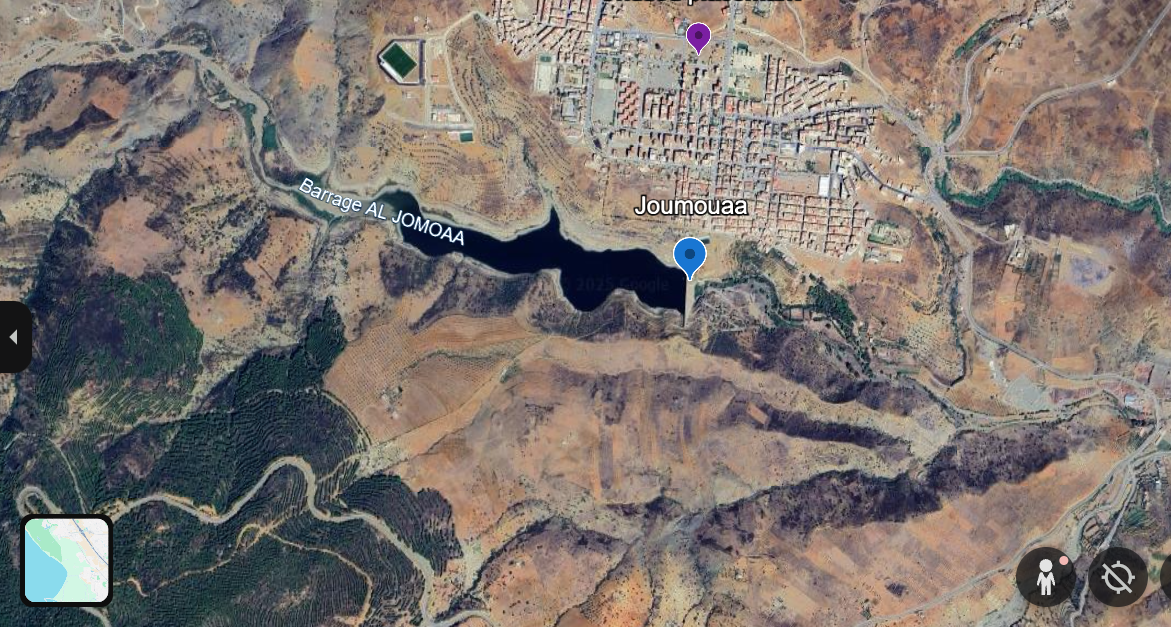
\includegraphics[width=\linewidth]{figures/joumaa}
    \end{graphicalabstract}

    % Research highlights
    \begin{highlights}
        \item Dam sites 18, 19, 20, and 28 appear most often in the results, making them reliable choices for Morocco's urgent dam site expansion needs.
        \item The four GP models (\gls{WGP}, \gls{LGP}, \gls{CGP}, \gls{EGP}) were extended with Multi-Choice Goal Programming to reflect the reality of multiple targets and choices in decision-making.
        \item Goal programming was adopted for its closeness in underlying principles with Collective Intelligence.
    \end{highlights}

    \begin{keyword}
        Multi-Criteria Decision-Making \sep Goal Programming \sep Dam Site Selection \sep Water Resource Management \sep Morocco
    \end{keyword}

\end{frontmatter}   
  

    \tableofcontents
    \clearpage
    \listoffigures
    \clearpage
    \listoftables
    \clearpage
    
    % \gls{GNU}
    % \glsaddall
    % \printnoidxglossaries
    % \printglossary[type=\acronymtype]
    % \begin{nolinenumbers}
    \nolinenumbers
    \glsaddall
     {\small
        \begin{multicols}{2}
        \printnoidxglossary[type=acronym]
        \end{multicols}}
    % \end{nolinenumbers}
    % \printacronyms


    \doublespacing

    %% The lineno packages adds line numbers. Start line numbering with
    %% \begin{linenumbers}, end it with \end{linenumbers}. Or switch it on
    %% for the whole article with \linenumbers.
    %% \usepackage{lineno}

    % \linenumbers

    \acresetall

    \section{Chapter 1 - Introduction}\label{sec:introduction}
Water has become one of the most strategically important and contested natural resources of the 21st century. Increasing population growth, accelerating urbanization, and the intensifying effects of climate change are exerting significant pressure on freshwater systems worldwide (American Meteorological Society 2017)\cite{AMS2017}. Dams have historically played a critical role in water management, providing storage for irrigation, hydropower generation, domestic supply, and flood control. Globally, they are regarded as cornerstones of national development strategies, yet their design and expansion decisions require careful balancing of social, economic, and environmental considerations \cite{Schmitt2024,AMS2017}.

In North Africa, and particularly in Morocco, the challenge of water scarcity is especially pronounced. Morocco is among the most water-stressed countries in the region, with per capita renewable water resources steadily declining over the last decades—from about $2,560m_3$ in 1960 to roughly $620m_3$ in 2020—due to reduced rainfall, rising demand, and sedimentation in existing reservoirs \cite{WorldBank2023}. Dams remain central to Morocco's national water policy, as they underpin agricultural productivity, food security, and energy diversification. The government has therefore invested heavily in dam infrastructure expansion, with over 150 large dams already constructed, and several additional projects planned \cite{TradeGov2024}. However, the benefits of such infrastructure are accompanied by substantial trade-offs related to land use, environmental sustainability, and local socio-economic impacts.

Selecting suitable sites for future dams thus constitutes a complex strategic decision problem. Beyond hydrological and engineering feasibility, the siting of dams must also account for population distribution, access to transport networks, farmland protection, and broader ecological constraints. Conventional single-objective approaches often fall short in capturing these competing dimensions. As a result, there has been a shift toward multi-criteria decision-making (MCDM) methods, which provide structured frameworks to integrate diverse quantitative and qualitative factors into dam site evaluations \cite{TradeGov2024,Minatour2015}. In this study, we position dam site selection  for expansion in Morocco within this broader discourse of sustainable and multi-objective water infrastructure planning.

\subsection{Problem of Dam Site Selection}
While dams are vital for Morocco's long-term water security and economic growth, the process of selecting their sites involves a web of conflicting objectives and constraints. On one hand, governments and planners seek to maximize storage capacity, agricultural productivity, and energy generation. On the other, environmental and social considerations, such as farmland preservation, displacement risks, ecological integrity, and equitable access, place strong constraints on dam siting decisions \cite{Wang2021,Zerdeb2025}. These competing goals transform site selection from a straightforward engineering task into a multi-objective decision problem that requires balancing diverse interests under uncertainty.

Traditional approaches to dam site evaluation have often prioritized hydrological suitability or cost efficiency, using single-objective models that emphasize technical feasibility. However, these methods tend to underrepresent the wider social and environmental impacts, leading to decisions that may be technically sound but socially or ecologically unsustainable. To overcome these limitations, researchers and practitioners have increasingly adopted multi-criteria decision-making (MCDM) frameworks, which explicitly incorporate heterogeneous factors into decision analysis \cite{Wang2021,Hagos2022}. MCDM methods enable decision makers to consider trade-offs among economic, environmental, and social criteria, while also accommodating input from multiple stakeholders.

In Morocco, these complexities are heightened by the diversity of candidate dam sites and the country's urgent need for expansion under resource constraints. From the 28 candidate sites considered in this study, three could be selected, making the optimization problem both discrete and sensitive to value judgments about which criteria should dominate. This tension underscores the importance of adopting robust decision-support tools capable of producing transparent, justifiable, and adaptable recommendations. It is in this context that the present work turns to \gls{GP}, a family of MCDM techniques especially suited to structuring and solving problems where multiple, potentially conflicting objectives must be addressed simultaneously.

\subsection{Multi-Criteria Decision-Making}
Decision-making in real-world contexts rarely revolves around a single objective. Governments, businesses, and communities are frequently confronted with situations where they must balance conflicting goals—for example, maximizing economic returns while minimizing environmental damage, or ensuring technical efficiency while promoting social equity. To address such complexities, scholars and practitioners have developed Multi-Criteria Decision-Making (MCDM) as a structured scientific approach that enables systematic evaluation of alternatives when trade-offs are unavoidable \cite{Aruldoss2013,Taherdoost2023}. Far from being a purely theoretical construct, MCDM has become a practical decision-support tool that reflects the realities of modern governance and resource management \cite{HUANG2011}.

At its core, Multi-Criteria Decision-Making (MCDM) refers to a family of quantitative and qualitative techniques designed to support decisions that involve multiple, often conflicting, evaluation criteria \cite{Aruldoss2013,Taherdoost2023}. Unlike simple optimization models, which concentrate on maximizing or minimizing a single objective, MCDM provides a structured way for decision-makers to balance competing priorities \cite{KUMAR2017596,jones2010}. In practice, this means that MCDM captures the reality that most real-world choices are about trade-offs rather than absolutes. In this sense, it can be seen as a form of collective reasoning: just as a group of individuals brings diverse perspectives to arrive at a shared judgment, MCDM integrates diverse evaluation criteria into a coherent and balanced decision outcome \cite{Borges2020,Cinalli2015}.

Over time, Multi-Criteria Decision-Making (MCDM) has developed into an interdisciplinary field, drawing insights from mathematics, economics, computer science, and the social sciences. The rapid growth of computational power has accelerated this evolution, making it possible to design more sophisticated approaches. In particular, fuzzy MCDM methods have been introduced to address uncertainty in decision environments \cite{LIANG1999,Mardani2015}, while hybrid approaches now integrate MCDM with artificial intelligence and machine learning to enhance accuracy and adaptability \cite{karakus2022}. As a result, MCDM has moved beyond being a theoretical tool to become a cornerstone of modern decision science, widely applied to some of today’s most complex real-world challenges.

MCDM techniques have demonstrated remarkable versatility across diverse fields. In engineering and environmental planning, they provide structured frameworks for prioritizing design alternatives and evaluating trade-offs in infrastructure development, environmental impact assessments, and land-use planning \cite{karakus2022,Dirie2024}. MCDM has been employed in energy systems to compare renewable energy technologies, identify suitable sites for facilities, and support the transition toward low-carbon strategies \cite{POHEKAR2004}. Business and finance also has use cases in assisting managers in evaluating investment portfolios, assessing operational risks, and formulating strategic policies \cite{TAMIZ1998}. Beyond these traditional domains, MCDM has also become increasingly prominent in sustainability research, where decision-makers must balance economic growth, ecological preservation, and social welfare in an integrated manner \cite{ettazarini2021,Mardani2015}. Collectively, these applications illustrate how MCDM adapts to the specific needs of each context while maintaining its role as a systematic tool for rational decision-making.

These applications highlight the very nature of the challenges MCDM is designed to address: decisions with multiple stakeholders, competing objectives, incomplete information, and long-term uncertainties. In this sense, MCDM resonates with the philosophy of collective intelligence, where diverse contributions must be synthesized into a coherent solution\cite{Cinalli2015}. Just as collective intelligence seeks to prevent dominance by a single actor in group decision-making, MCDM provides a safeguard against the dominance of a single criterion in technical evaluations. This parallel underscores MCDM's role not only as a computational tool but also as a conceptual bridge between quantitative rigor and inclusive decision-making.   

The importance of MCDM has grown in recent decades due to the increasing complexity of global challenges. Climate change, resource scarcity, and sustainable development goals all require decisions that balance competing priorities. For instance, governments must decide how to allocate limited water supplies across agriculture, energy, and domestic use; companies must balance profitability against environmental and social responsibility; and communities must weigh development needs against cultural and ecological preservation \cite{KUMAR2017596,PortnerIPCC2022}. Traditional single-objective decision tools fall short in these contexts, while MCDM offers a structured and transparent process for evaluating trade-offs.

MCDM provides a rigorous yet flexible decision-support framework, particularly well-suited to wicked problems—those with no single optimal solution but multiple competing pathways. This makes it a powerful tool for addressing Morocco's dam site investment challenge, where economic, social, and environmental goals must all be considered simultaneously under conditions of uncertainty.

\subsection{MCDM in Water Resource Management and Dam Site Selection}
The complexity of water resource management makes it a prominent field for the application of Multi-Criteria Decision-Making (MCDM). Early studies in this domain emphasized technical and economic feasibility, particularly in irrigation planning, watershed management, and hydropower development \cite{POHEKAR2004,Romanelli2018}. However, these approaches often overlooked environmental and social dimensions, limiting their comprehensiveness.

From the mid-2000s onward, the literature reflects a growing integration of Geographic Information Systems (GIS) with MCDM to enable spatially explicit decision frameworks. For example, \cite{Romanelli2018} combined GIS and AHP to identify hydropower locations in Brazil, while \cite{karakus2022} applied GIS-based multi-criteria analysis for dam site suitability in Turkey. These studies highlighted how spatial integration of hydrological, geological, and socio-economic data strengthens the robustness of site evaluations.

Uncertainty in hydrological and climate conditions has also driven the development of fuzzy and probabilistic MCDM methods. \cite{LIANG1999} pioneered fuzzy extensions of MCDM based on ideal and anti-ideal concepts, and subsequent reviews \cite{Mardani2015} show that fuzzy MCDM techniques have become widely used for handling ambiguity in water resource allocation and dam planning. Recent studies extend this trend by employing hybrid models that combine MCDM with optimization algorithms or artificial intelligence. \cite{PHAM2021}, for instance, integrated hybrid artificial intelligence models with multi-criteria decision analysis to improve flood risk assessment in Vietnam.

The evolution of criteria in dam site selection is another clear trend. While early models emphasized economic and engineering parameters, contemporary studies increasingly incorporate environmental and social concerns such as biodiversity protection, resettlement impacts, and ecosystem trade-offs \cite{Dirie2024,karakus2022}. Reviews of the literature highlights four broad developments. The widespread adoption of GIS for spatial analysis, a shift toward sustainability criteria alongside engineering and economic factors, expanded use of fuzzy and probabilistic approaches to address uncertainty, and the integration of MCDM with machine learning and optimization for greater accuracy.

Despite these advances, several gaps persist. The selection and weighting of criteria remain highly subjective and context-dependent, creating challenges for replicability \cite{Belton2002,Mardani2015}. Data scarcity, especially in developing regions, further constrains model precision and reliability \cite{POHEKAR2004,Dirie2024}. Moreover, most studies emphasize projects such as new dams or small hydropower, while fewer address the optimization of existing infrastructure, which is equally critical under climate and fiscal constraints \cite{KUMAR2017596,Romanelli2018}. Finally, there is limited application of these frameworks in North African contexts, despite acute water scarcity and reliance on dams in countries such as Morocco \cite{ettazarini2021}.

This gap is particularly significant for Morocco, where the central challenge is not simply the identification of new dam sites but the prioritization of existing infrastructure for expansion and rehabilitation under competing economic, environmental, and social pressures. Addressing this gap requires the adoption of systematic, context-specific MCDM frameworks that explicitly integrate sustainability goals with fiscal and climate realities.

\subsection{Collective Intelligence in MCDM}
Multi-Criteria Decision-Making MCDM offers a family of methodologies—ranging from value measurement methods such as the Analytic Hierarchy Process (AHP) and Analytic Network Process (ANP), to outranking methods such as \gls{ELECTRE} and \gls{PROMETHEE}, to distance-based techniques like \gls{TOPSIS}, and to mathematical programming approaches such as \gls{GP} and Multi-Objective Linear Programming (MOLP)\cite{Belton2002,Aruldoss2013}. Each methodology provides a different mechanism for balancing conflicting objectives: value measurement methods rely on hierarchical structuring and subjective weights, outranking methods emphasize pairwise comparison and preference thresholds, distance-based approaches compare alternatives to ideal/anti-ideal solutions, and mathematical programming models optimize across multiple objectives under explicit constraints.

Theories of CI, as discussed by \cite{Woolley2010}, highlight that groups outperform individuals when three conditions are met: diversity of perspectives, independence of judgments, and effective aggregation mechanisms. When viewed through this lens, MCDM methodologies can be understood as formal aggregation mechanisms that operationalize these principles. AHP and ANP capture diversity through structured weighting, outranking methods allow pluralism of thresholds and vetoes, and fuzzy/gray extensions address uncertainty in human judgments \cite{Mardani2015,LIANG1999}. However, most of these methods are either too dependent on subjective weights or lack iterative feedback loops that resemble the adaptive, deliberative, and iterative nature of CI systems \cite{Cinalli2015}.

 \gls{GP} stands out as the MCDM methodology most aligned with CI theories. Like collective intelligence, \gls{GP} does not aim for a single optimal solution but rather for a 'satisficing' compromise that balances multiple, often conflicting, goals. Just as groups rarely arrive at unanimous “optimal” outcomes but instead reach negotiated compromises through deliberation, \gls{GP} models minimize deviations from a set of priority-ranked or weighted goals rather than forcing one criterion to dominate \cite{jones2010}. Moreover, \gls{GP} frameworks are inherently flexible: they allow the integration of diverse stakeholder goals, adjustment of priorities, and iterative recalibration—mirroring the feedback-driven and inclusive character of collective intelligence processes \cite{Borges2020}.

While many MCDM methods resonate with elements of CI,  is the methodology that most closely embodies its spirit, particularly in contexts where diverse goals must be reconciled rather than hierarchically imposed. For this reason, our study adopts four distinct  models—Weighted  \gls{WGP}, Compromise  \gls{CGP}, Extended  \gls{EGP}, and \gls{LGP}, to investigate how different compromise structures capture the dynamics of collective decision-making in complex, multi-criteria contexts.

\subsection{Goal Programming}
\gls{GP} is particularly well suited for addressing complex infrastructure planning problems such as dam site selection, where multiple and often conflicting objectives must be balanced. Unlike single-objective optimization, which collapses diverse concerns into a single aggregate function, \gls{GP} preserves the multidimensional nature of decision-making \cite{CHANG2007}. It does so by minimizing deviations from multiple goals, thereby offering solutions that reflect a compromise among technical, economic, environmental, and social considerations. In recent years, \gls{GP} models have been applied in contexts with strong stakeholder conflicts and ecological constraints, creating more sustainable decision pathways \cite{Castro2021}.

A further advantage of \gls{GP} lies in its flexibility. The method allows for different formulations that align with distinct decision‑making philosophies. The \gls{WGP} model facilitates explicit trade-offs between goals through assigned weights, making it well suited for contexts where objectives can be expressed in relative importance \cite{JONES2011}. \gls{LGP}, by contrast, imposes a strict hierarchy of priorities, ensuring that higher-order goals are fully satisfied before lower-order ones are considered \cite{jones2010}. \gls{CGP} emphasizes fairness by minimizing the maximum deviation across all goals, producing outcomes that are more equitable among competing objectives \cite{JONES2011}. Finally, the \gls{EGP} model generalizes the \gls{GP} framework by introducing additional parameters that penalize deviations asymmetrically, thereby capturing flexible stakeholder preferences and allowing more nuanced solutions \cite{jones2010}

Taken together, these four formulations enable decision makers to examine the dam site selection problem through multiple lenses: balanced compromise \gls{WGP}, priority satisfaction \gls{LGP}, fairness \gls{CGP}, and flexibility \gls{EGP}. In this study, each formulation is mapped to a distinct sub-question concerning how Morocco's dam expansion strategy might weigh competing objectives. By doing so, the analysis not only identifies feasible dam site combinations, but also generates a spectrum of alternatives reflecting different governance and policy orientations. This multimodel approach also strengthens the robustness of final recommendations, as it allows comparisons across frameworks and provides insights into the conditions under which different dam sites emerge as optimal.



    \section{Chapter 2 - Methodology}\label{sec:methodology}

\subsection*{Research Objectives and Sub-Questions}
The overarching objective of this research is to support evidence-based dam site selection 
for Morocco’s future water infrastructure expansion, under conditions of competing 
economic, social, environmental, and technical objectives. Specifically, the study addresses the challenge of selecting three sites from a pool of 28 candidate dams, while ensuring that the solutions remain robust, transparent, and adaptable to shifting policy priorities.

To operationalize this objective, the study applies four Goal Programming (GP) formulations, 
each addressing a distinct sub-question:

\begin{itemize}
    \item \textbf{Weighted Goal Programming (WGP):} What is the most balanced solution when 
    objectives are explicitly weighted according to their relative      ?
    \item \textbf{Lexicographic Goal Programming (LGP):} What solution emerges when objectives 
    are ranked hierarchically and pursued in strict priority order?
    \item \textbf{Chebyshev Goal Programming (CGP):} How can the selection be made fair by 
    minimizing the maximum deviation across all objectives?
    \item \textbf{Extended Goal Programming (EGP):} How do flexible formulations, which 
    penalize deviations asymmetrically, alter site selection when stakeholder preferences 
    are uneven?
\end{itemize}

In addition to these base models, the research incorporates Multi-Choice Goal Programming (MCGP) extensions, which allow for more realistic goal setting by considering intervals or multiple aspiration levels rather than fixed targets. This extension captures the uncertainty and diversity of stakeholder preferences, broadening the scope of feasible solutions.

Finally, a Sensitivity Analysis (SA) is performed on both weights and targets to 
evaluate the robustness and reliability of the proposed solutions. The SA addresses questions 
such as: \textit{How stable are the selected dam sites under changing weight assignments?} and 
\textit{Which dams remain consistently selected across different target scenarios?}

\subsection{Criteria Selection}
The robustness of any Multi-Criteria Decision-Making (MCDM) model depends fundamentally on the choice of evaluation criteria, since these define the dimensions along which dam sites are assessed. The inclusion or exclusion of particular indicators can significantly influence outcomes, as previous studies on dam planning have demonstrated \cite{Roudgarmi2019}. In this study, ten criteria were selected to evaluate and prioritize dam sites for investment in Morocco, combining technical, environmental, socio-economic, and infrastructural dimensions to ensure a balanced assessment. Table 1 summarizes these criteria, their units, data sources, and justifications.

Technical indicators such as dam height, storage capacity, and reservoir area were included because they determine the physical potential of a site to store water. These measures are widely used in hydropower site selection literature and remain fundamental in investment decisions \cite{MOIZ2018309,Rana2020}. Climatic conditions, represented by temperature and rainfall, provide essential insight into the sustainability of storage and inflows. High temperatures intensify evaporation losses, while rainfall history indicates hydrological reliability, both of which are critical under Morocco’s variable climate \cite{Belokda2018}.

Socio-economic dimensions were captured by commune population, proximity to residential centers, farmland area, and farmland distance. Population reflects demand pressure and potential beneficiaries, though normalization was conducted to prevent large communes from skewing results \cite{Ersoy2022,Kosareva2018}. Likewise, farmland measures account for the agricultural benefits of dam expansion, emphasizing the role of irrigation in Morocco’s water strategy \cite{Ghumman2020}. Proximity to settlements ensures accessibility and equity, aligning with social sustainability goals.

Infrastructural connectivity, represented by the distance to the nearest road, was included because access routes directly affect construction costs, operational efficiency, and maintenance feasibility \cite{YI2010852}. Together, these ten dimensions ensure that the analysis captures Morocco’s triple objective: meeting water demand, ensuring economic returns, and promoting long-term sustainability.

To estimate the targets for each criterion, the model maximizes values under the constraint of selecting three dams with a total budget of 500 million USD. The maximum achievable objective then serves as the benchmark or “target.” This approach ensures that the targets are not arbitrary but instead reflect realistic upper bounds within fiscal and operational constraints.

Insights from prior studies further underscore the importance of such criteria design. For instance, Rana and Patel (2020) demonstrated that including population data shifted site rankings compared to purely technical models \cite{Rana2020}, while \cite{TEMEL2023159152} showed that incorporating ecological considerations produced different priorities than cost-based evaluations alone . These findings confirm that criteria selection fundamentally shapes decision outcomes.

The ten selected criteria provide a comprehensive and context-appropriate framework for evaluating Morocco’s dams. By incorporating physical, climatic, social, and infrastructural factors (see Table 1), the study ensures methodological rigor while reflecting principles of collective intelligence.

\subsection{Data Source}
% --------------
Hydrological and structural attributes of dams were obtained from the Food and Agriculture Organization (FAO) AQUASTAT database for Morocco \cite{FAO_AQUASTAT_MAR}. Dam height is reported in meters (m) and refers to the vertical distance from the crest to the lowest foundation point. Storage capacity is measured in million cubic meters (10\textsuperscript{6} m\textsuperscript{3}) and reflects the initial designed volume of the reservoir, not considering reduction due to sedimentation. Reservoir surface area is reported in square kilometers (km\textsuperscript{2}) and shows the water-covered footprint when the reservoir is at full supply level.

Climatic data were sourced from the NASA POWER database \cite{NASA_POWER_API}, which provides historical rainfall and temperature records. For each dam-site commune, monthly values from 2010 to 2024 were aggregated into annual totals, and the median annual values were taken as representative estimates. Rainfall is expressed in millimeters per year (mm/year), while temperature is measured in degrees Celsius (°C).

Socio-economic and land-use indicators were extracted from shapefiles obtained from SIG-Maroc \cite{SIG_Maroc_Shapefiles} and processed with QGIS and Python. Commune population provides an estimate of the number of residents living in the same commune as the dam site. Because population values varied widely (range: 1,276–1,494,413; span: 1,493,137) \cite{Ersoy2022}, the data were normalized using min–max scaling into a 0–50 range to reduce the influence of extremes \cite{Kosareva2018,population_normalization_py}. Distance to the nearest road was calculated in kilometers (km) using geographical coordinates of each dam \cite{Coordinates2025}, provincial route shapefiles \cite{routes2025}, and the Python GeoPandas package \cite{roadsCode2025}. Farmland area was derived from land use/land cover (LULC) shapefiles \cite{LULC_MegaArchive} and estimated in square meters (m\textsuperscript{2}), while farmland distance was calculated as the shortest distance between the dam-site centroid and the closest farmland polygon \cite{farmlandAreaCode2025}.

Finally, nearest conglomerate residence — defined as the shortest distance between the dam site and the nearest highly populated settlement — was estimated by visual inspection of Google Earth imagery \cite{congolerateResidenceGearth2025}, combined with distance calculations using the Geopy Python package \cite{congloResidence2025}.

\begin{table}[!ht]
\centering
\caption{Summary of Criteria and Data Sources}
\begin{tabular}{|p{4cm}|p{3.5cm}|p{2.5cm}|p{4cm}|}
\hline
\textbf{Criterion} & \textbf{Data Source} & \textbf{Unit} & \textbf{Processing Notes} \\
\hline
Dam height & FAO AQUASTAT \cite{FAO_AQUASTAT_MAR} & Meters & Direct extraction from national database \\
\hline
Reservoir storage capacity & FAO AQUASTAT \cite{FAO_AQUASTAT_MAR} & Million m$^3$ & Used as initial reservoir volume \\
\hline
Reservoir surface area & FAO AQUASTAT \cite{FAO_AQUASTAT_MAR} & km$^2$ & Used to assess spatial footprint \\
\hline
Annual rainfall (median) & NASA POWER \cite{NASA_POWER_API} & mm/year & Aggregated from monthly data (2010–2024) \\
\hline
Annual temperature (median) & NASA POWER \cite{NASA_POWER_API} & °C & Aggregated from monthly data (2010–2024) \\
\hline
Commune population & SIG-Maroc \cite{SIG_Maroc_Shapefiles} & Persons & Derived from shapefiles; normalized via min–max scaling \\
\hline
Distance to nearest road & SIG-Maroc \cite{SIG_Maroc_Shapefiles} & Kilometers & Calculated using GeoPandas and provincial road shapefiles \\
\hline
Farmland area & LULC Archive \cite{LULC_MegaArchive} & m$^2$ & Extracted from LULC shapefiles via geospatial processing \\
\hline
Distance to farmland & LULC Archive \cite{LULC_MegaArchive} & Kilometers & Spatially computed from dam-site centroid \\
\hline
Distance to nearest conglomerate residence & Google Earth + Geopy \cite{congloResidence2025} & Kilometers & Visual inspection + spatial computation using Python \\
\hline
\end{tabular}
\label{tab:data_sources}
\end{table}


\subsection{Goal Porgramming Variants}

A generic goal program \cite{jones2010} may be presented as:

Minimize:
            \EqGGPMinFunctionOne
Subject to:
            \EqGGPMinFunctionSubTwo
            \EqGGPMinFunctionSubThree
            \EqGGPMinFunctionSubFour    

The generic Goal Programme has Q goals involving n decision variables $x = x_1,x_2, ...,x_n.$ Each goal $q$ has a target value $b_q$ and an acheived value $f_q(x)$. Each goal then has a positive or negative deviational varibales $p_q$ and $n_q$ respectively. $p_q$ and $n_q$ are non-negative and cannot be non-zero simultaneously. $h$ is a function of the deviational variables representing the penalties associated with non-acheivement of the targets and R is the feasible region of $x$ in decision space.

\subsection{Weighted Goal Programming}
In Weighted Goal Programming (WGP) the objective function is a simple sum of the deviational variables by allocating suitable weigts to each of them (the $L_1 $ metric). \cite{jones2010} recommend normalisation and assuming that $b_q > 0 \qquad q = 1, ..., Q$, the model becomes:

Minimize:
            \EqWGPMinFunctionFive
Subject to:
            \EqGGPMinFunctionSubTwo
            \EqGGPMinFunctionSubThree
            \EqGGPMinFunctionSubFour
Where $R$ is the feasible region of $x$ in the decision space.

We apply this base model to our dam site expansion project as follows:

Minimise:
        \EqDamWGPObjectiveEleven

Subject to:
        \EqDamHeightConstraintTwelve
        \EqDamCapacityConstraintThirteen
        \EqReservoirAreaConstraintFourteen
        \EqTemperatureConstraintFifteen
        \EqPopulationConstraintSixteen
        \EqRainfallConstraintSeventeen
        \EqResidenceConstraintEighteen
        \EqFarmlandDistanceConstraintNineteen
        \EqNearestRoadConstraintTwenty
        \EqFarmlandAreaConstraintTwentyOne
        \EqSelectThreeDamsTwentyTwo
        \EqBudgetConstraintTwentyThree

Similarly, the objective function Equation~$9$ has 10 terms, each representing a criteria. The function is minimizing all terms, which comprise of positive ($p_3,p_4,p_7,p_8,p_9$) and negative ($n_1,n_2,n_5,n_6,n_10$) deviations. For now, all terms are equally weighted (1). $h_i, c_i, r_i, t_i, pop_i, rain_i, res_i, d_i, road_i$ and $a_i$ represent the 10 criteria, dam height, reservoir storage capacity reservoir surface area, ,  annual temperature,   commune population, annual rainfall, disance to nearest conglomerate residence, distance to farmland, distance to nearest road, and farmland area respectively. Equations~$20$ and $21$
represent the selections and budget constrains, where $x_i$ is binary and  $b_i$ is in millions of dollars.

\subsection{Chebyshev Goal Programming}
In Chebyshev Goal Programming (CGP) the objective is to minimize the maximum deviation of the goal. The CGP was first used by Flavell \cite{FLAVELL1976} but more recent examples are given in \cite{Despotis2008,HO2019}. This minmax criteria uses the $L_\infty$ metric and aims to achieve a balance between the different levels of the statisfaction of each of the goals. The model is defined as:

Minimize:
            \EqCGPMinFunctionSix
Subject to:
            \EqGGPMinFunctionSubTwo
            \EqCGPConstraintSeven
            \EqCGPConstraintEight
            \EqGGPMinFunctionSubFour
            \EqCGPConstraintNine

All variables non-negative. In the base Chebyshev Goal Programming (GP) model, the decision vector is denoted by $x$, which belongs to the feasible set $F$. For each goal $q=1,\dots,Q$, the achievement function is represented by $f_q(x)$ with the corresponding aspiration level $b_q$. The variables $n_q$ and $p_q$ denote the negative and positive deviations from the $q$-th goal, respectively. The parameters $u_q$ and $v_q$ are the weights assigned to the negative and positive deviations, reflecting their relative importance. The scalar $D$ represents the maximum weighted deviation, i.e., the Chebyshev distance to be minimized. Finally, $Q$ indicates the total number of goals considered in the model.

We apply this base model to our dam site expansion project as follows:

Minimise:
            \EqCGPMinFunctionSix
Subject to:
            \EqDamHeightConstraintTwelve
            \EqDamCapacityConstraintThirteen
            \EqReservoirAreaConstraintFourteen
            \EqTemperatureConstraintFifteen
            \EqPopulationConstraintSixteen
            \EqRainfallConstraintSeventeen
            \EqResidenceConstraintEighteen
            \EqFarmlandDistanceConstraintNineteen
            \EqNearestRoadConstraintTwenty
            \EqFarmlandAreaConstraintTwentyOne
            \EqSelectThreeDamsTwentyTwo
            \EqBudgetConstraintTwentyThree
            \EqDConstraintOneNTwentyFour
            \EqDConstraintTwoNTwentyFive
            \EqDConstraintThreeNTwentySix
            \EqDConstraintFourNTwentySix
            \EqDConstraintFiveNTwentySeven
            \EqDConstraintSixNTwentyEight
            \EqDConstraintSevenNTwentyNine
            \EqDConstraintEightNThirty
            \EqDConstraintNineNThirtyOne
            \EqDConstraintTenNThirtyTwo

\subsection{Extended Goal Programming}  
Extended Goal programming (EGP) was first proposed by Romero \cite{ROMERO2001} in the context of a lexicographic ordering of the goals and was later generalised in \cite{ROMERO2004}. Some recent applications include \cite{Guijarro2018,Pal2014}. It aims to allow both of the above approaches by combining the optimisation given by WGP and the balancing given by CGP. For a nonlexicographic EGP, the general model is:


Minimise:
            \EqEGPMinFunctionTen
Subject to:
            \EqGGPMinFunctionSubTwo
            \EqCGPConstraintSeven
            \EqCGPConstraintEight
            \EqGGPMinFunctionSubFour
            \EqCGPConstraintNine
The parameter $\alpha$ is a constant between 0 and 1 which controls the mix of optimization ($L_1$)and balance ($L_\infty$) in the acheivement function.
Similarly in the EGP model, the decision vector is denoted by $x$, restricted to the feasible set $F$. The achievement function for each goal $q=1,\dots,Q$ is given by $f_q(x)$ with the aspiration level $b_q$. The variables $n_q$ and $p_q$ measure the negative and positive deviations from the $q$-th goal, respectively, while $u_q$ and $v_q$ denote their corresponding importance weights. The parameter $\alpha \in [0,1]$ controls the balance between minimizing the maximum weighted deviation, represented by $D$, and minimizing the sum of normalized weighted deviations across all goals. 
Thus, the objective function $\alpha D + (1-\alpha)\sum_{q=1}^{Q}\left(\tfrac{u_q n_q}{b_q}+\tfrac{v_q p_q}{b_q}\right)$ combines the Chebyshev distance with the weighted $L_1$ norm, offering a compromise between efficiency and balance in goal satisfaction. Finally, $Q$ is the total number of goals in the model.


Dam site selection for expansion, Extended Goal Program Formulation:

Minimise:
        \EqEGPObjectiveThirtyThree

Subject to:
            \EqDamHeightConstraintTwelve
            \EqDamCapacityConstraintThirteen
            \EqReservoirAreaConstraintFourteen
            \EqTemperatureConstraintFifteen
            \EqPopulationConstraintSixteen
            \EqRainfallConstraintSeventeen
            \EqResidenceConstraintEighteen
            \EqFarmlandDistanceConstraintNineteen
            \EqNearestRoadConstraintTwenty
            \EqFarmlandAreaConstraintTwentyOne
            \EqSelectThreeDamsTwentyTwo
            \EqBudgetConstraintTwentyThree
            \EqDConstraintOneNTwentyFour
            \EqDConstraintTwoNTwentyFive
            \EqDConstraintThreeNTwentySix
            \EqDConstraintFourNTwentySix
            \EqDConstraintFiveNTwentySeven
            \EqDConstraintSixNTwentyEight
            \EqDConstraintSevenNTwentyNine
            \EqDConstraintEightNThirty
            \EqDConstraintNineNThirtyOne
            \EqDConstraintTenNThirtyTwo

\subsection{Lexicographic Goal Programming}

To formulate the lexicographic goal program algebraically, we define the number of priority levels as $L$ with corresponding index $l = 1, ..., L.$ Each priority level now becomes a function of a set of unwanted deviational variables which we define as $h_1(n, p)$, giving the equation below:

Minimize:
            \EqLObjectiveThirtyThree
Subject to:
            \EqGGPMinFunctionSubTwo
            \EqCGPConstraintEight
            \EqGGPMinFunctionSubFour   

where each $h_1(n,p)$ contains a number of unwanted deviational variables. The exact nature of $h_1(n,p)$ depends on the nature of the goal programme to be formulated, but if we assume that it is linear and separable then it will assume the form 

            \EqLObjectiveThirtyFour

Where $u_q^l$ is the preferential weight associated with the minimisation of $n_q$ in the $l$th priority level. $v_q^l$ is the preferential weight associated with the minimisation of $p_q$ in the $l$th priority level. 

To model our problem using the Lexicographic Goal Programming, we group goals into three priority levels, priority level 1 (Dam Hieght, Dam Capacity, Population, and Farmland Area), priority level 2 (Reservoir Area, Temperature, and Rainfall), and priority level 3 (Residence distance,Farmland distance, and Nearest road distance). In this caterization, we consider the goals in the first priority level as infinitely more important than goal in lower levels.
In practice, this means that the optimization first focuses on minimizing deviations for the goals in priority level 1. Only after the best possible achievement of these goals is secured do we consider the goals in priority level 2, and subsequently priority level 3. At each stage, the solution space is restricted so that improvements at lower levels never come at the expense of higher-level goals. This hierarchical structure reflects the decision makers' preferences, ensuring that the most critical objectives dominate the solution process.

Let $P_1$ and $P_2$ be the objective function values for Priority 1 and Priority 2, the EqLGPObjectivePriorityThreeThirtySeven model can be expressed as follows:
Priority one (1) Model:

Minimize:
        \EqLGPObjectivePriorityOneThirtyFive

Subject to:

       \begin{center}
        Equations ~$28$ to ~$50$
        \end{center}  
Priority two (2) Model:

Minimise:
        \EqLGPObjectivePriorityTwoThirtySix

Subject to:
         \begin{center}
        Equations ~$28$ to ~$50$
        \end{center}  
        \EqLGPObjectivePriorityOneConstraintThirtyEight

Priority three (3) Model:

Minimise:
        \EqLGPObjectivePriorityThreeThirtySeven

Subject to:
        \begin{center}
        Equations ~$28$ to ~$50$
        \end{center}   
        \EqLGPObjectivePriorityOneConstraintThirtyEight
        \EqLGPObjectivePriorityTwoConstraintThirtyNine

\subsection{Multi-Choice Goal Programming}
In traditional goal programming, a decision maker specifies a single aspiration level for each goal. For example, a target profit, a desired level or service, or environmental impact. The model then seeks to minimize the difference between what is acheived and this single target.

However, in many real-world problems, it is unrealistic to think that there is only one acceptable target. Decision Makers may instead face a situation where several possible aspiration levels are reasonable. For example, a company might aim for at least \$1M in profit, but would also be satisfied if it reaches \$1.2M or \$1.3M. Similarly, a community might consider different acceptable levels of water storage or pollution reduction.

This is where Multi-Choice Goal Programming (MCGP) comes in. Instead of fixing just one aspiration level per goal, MCGP allows multiple aspiration levels to be set. The model then chooses the most appropriate level during optimization, depending on what is feasible given the constraints. This flexibility better reflects the real uncertainty and negotiation invloved in decision making.

MCGP General Formulation

The general idea of the MCGP can be written as \cite{CHANG2007}:

Minimise:
       \EqMCGPObjectiveFourty

Subject to:
       \EqMCGPConstraintFourtyOne

Where:
\begin{itemize}
  \item $f_i(X)$ is the achievement of goal $i$
  \item $g_ij$ is one of the possible aspiration levels for goal i
  \item $d_i^+$ and $d_i^-$ are the over-archievement deviations
  \item $z_ij$ is a binary variable that selects which aspiration level is chosen for goal $i$
  \item $X$ is the set of decision varibales subject to feasiblity constraints.
\end{itemize}
Under each goal, the model not only minimizes deviations but also chooses which level among the multiple options is best matched under the given conditions.

\subsection{Applying Multi-Choice Goal Programming}

The concept of Multi-Choice Goal Programming is applied to Weigthed Goal Program model (WGP), Chebyshev Goal Program (CGP), and Extended Goal Program (EGP).
For our dam site selection project, 5 of the targets can be could assume multiple values. These are population, residence distance, farmland distance, nearest road, and farmland area. Thus, an extra goal value, which is 10 percent (10\%) more than the original goal is created for each.

\subsubsection{Multi-Choice Weighted Goal Program (MCWGP)}
To extend Weighted Goal program to multi-choice goal program, the orginal weigted goal program defined from equations ~$9$ to ~$21$ are maintained. The only change is in the targets of the constraints corresponding to population, residence distance, farmland distance, nearest road, and farmland area as showed below:

Minimise:
\EqDamWGPObjectiveEleven

Subject to:
        \EqMCWGPPopulationConstraintFourtyTwo   
        \EqMCWGPResidenceConstraintFourtyThree
        \EqMCWGPFarmlandDistanceConstraintFourtyFour
        \EqMCWGPNearestRoadConstraintFourtyFive
        \EqMCWGPFarmlandAreaConstraintFourtySix
        \begin{center}
               ~$9$ to ~$21$ 
        \end{center}


Where $ z_1, z_2, z_3, z_4$, and $z_5$ are binary vairables.

\subsubsection{Multi-Choice Chebyshev Goal Program (MCWGP)}
In a similar approach, we extend the Chebyshev Goal Program with the target flexibility of the multi-choice goal program. To acheive this, we maintain all equations of the the CGP and change the targets for population, residence, farmland, nearest road, and farm area constraints.

Minimize:
              \EqCGPMinFunctionSix

Subject to:
                
              \EqMCWGPPopulationConstraintFourtyTwo   
              \EqMCWGPResidenceConstraintFourtyThree
              \EqMCWGPFarmlandDistanceConstraintFourtyFour
              \EqMCWGPNearestRoadConstraintFourtyFive
              \EqMCWGPFarmlandAreaConstraintFourtySix
              \begin{center}
                      Equations ~$10$ to ~$21$ unchanged.
              \end{center}
              \EqSelectThreeDamsTwentyTwo
              \EqBudgetConstraintTwentyThree
              \EqDConstraintOneNTwentyFour
              \EqDConstraintTwoNTwentyFive
              \EqDConstraintThreeNTwentySix
              \EqDConstraintFourNTwentySix
              \EqDConstraintFiveNTwentySeven
              \EqDConstraintSixNTwentyEight
              \EqDConstraintSevenNTwentyNine
              \EqDConstraintEightNThirty
              \EqDConstraintNineNThirtyOne
              \EqDConstraintTenNThirtyTwo

Where $ z_1, z_2, z_3, z_4$, and $z_5$ are binary vairables.

\subsubsection{Multi-Choice Chebyshev Goal Program (MCWGP)}
In a similar way, an Extended Goal Programming version of weighted goal program would be the usual EGP with the targets of the appropriate goals modefied.

Minimise:
              \EqEGPObjectiveThirtyThree
Subjec to:
              \EqMCWGPPopulationConstraintFourtyTwo   
              \EqMCWGPResidenceConstraintFourtyThree
              \EqMCWGPFarmlandDistanceConstraintFourtyFour
              \EqMCWGPNearestRoadConstraintFourtyFive
              \EqMCWGPFarmlandAreaConstraintFourtySix
              \begin{center}
                      Equations ~$10$ to ~$21$ unchanged.
              \end{center}
              \EqSelectThreeDamsTwentyTwo
              \EqBudgetConstraintTwentyThree
              \EqDConstraintOneNTwentyFour
              \EqDConstraintTwoNTwentyFive
              \EqDConstraintThreeNTwentySix
              \EqDConstraintFourNTwentySix
              \EqDConstraintFiveNTwentySeven
              \EqDConstraintSixNTwentyEight
              \EqDConstraintSevenNTwentyNine
              \EqDConstraintEightNThirty
              \EqDConstraintNineNThirtyOne
              \EqDConstraintTenNThirtyTwo

\subsection{Sensitivity Analysis}
Dam site selection is inherently complex, characterized by multiple criteria whose influences are uncertain. Sensitivity Analysis (SA) accesses how variations in inputs affect model output\cite{Jakub2023}.

The objective of SA in this project is to to answer the question: How stable are the outcomes of the various site selection models?

\subsubsection{Sensitivity Analysis test data generation}
Two Sensitivity Analysis (SA) test are conducted, weighted analysis and target analysis. Weighted SA determines the effect of slight changes in weight to the outcomes of the models. It is conducted for Weighted GP and Lexicographic GP models. For WGP SA test, each term in the objecive function received a weight (decimal value between 0 and 1). All weight within a test weight set sum up to one(1). The model is ran 10 times with 10 different weight sets and he output recorded. Target analysis verifies how changes in targets affect the original outcome. It is conducted for all four models. Similarly, the models are ran 10 times with 10 different set of targets, each criteria receiving a different target value in each ran. All test are conducted keeping dam site selection number (3) and budget ($\$500M$) constant. This assumes no uncertainty in the proposed budget for constructing 3 dam sites.

10 weight sets, each for a term in the WGP model were generated using dirichlet sampling\cite{Neal2000}. The Dirichlet generator creates a uniformly distributed vector across the goal simplex. The Dirichlet distribution is a statistical tool used when you have several proportions that must add up to one. It’s the multi-category version of the Beta distribution and is often used in Bayesian modeling because of it's has convenient mathematical properties\cite{Lin2016}. Dirichlet sampling has been effectively used in modeling income-share distributions, portfolio weighting, and objective weighting\cite{khoi2025,Duangkamon2002,Williams2024}.

In MCDM, a moderate number of iterations is sufficient to capture stability patterns without overburdening computation. For instance, \cite{Triantaphyllou1997} highlight that sensitivity analysis in decision models does not require exhaustive runs; rather, a limited number of systematic variations can reveal whether rankings are robust to weight changes. Similarly, \cite{Belton2002} note that a relatively small set of scenarios (often 5–15) is adequate to detect meaningful changes in alternatives’ rankings. Therefore, conducting 10 rounds provides a balanced approach—enough to observe whether rankings shift under plausible weight variations, while keeping the analysis efficient.






















    \section{Chapter 3 - Results}\label{sec:results}

\subsection{Weighted Goal Programming Solution}
The model selected Dams 18, 19, and 23 with a total cost of \$481.5M. Relative to the ten goals, the solution exceeds several targets (e.g., height, capacity) while minimizing the weighted penalty of deviations, resulting in a weighted deviation score of 14.93. We can observe from Figure \ref{fig:wgpDeviationsChart} that the farmland area criterion was the driving factor in the WGP solution, with dam height and rainfall also exerting a significant influence. These three criteria together shaped the final weighted deviation score of 14.93. Table \ref{tab:model_results} lists per-dam attributes; Table \ref{tab:wgpAcheivementVsTarget}    summarizes achieved values versus targets and the corresponding deviations. This indicates a balanced compromise solution under the specified weights and budget.

\begin{figure}[htbp]
\centering
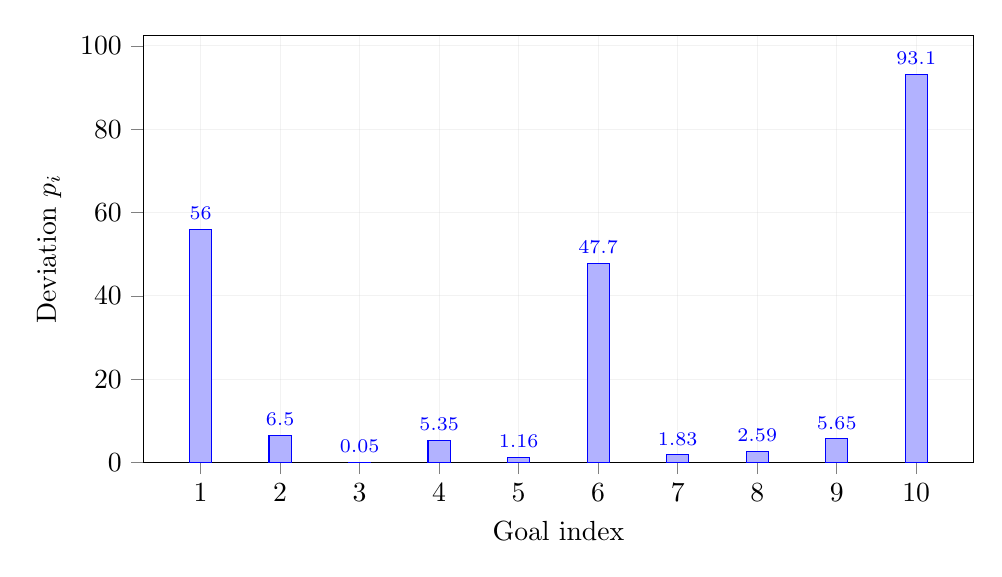
\begin{tikzpicture}
\begin{axis}[
    ybar,
    ymin=0,
    width=\textwidth,
    height=7cm,
    bar width=8pt,
    enlarge x limits=0.08,
    ylabel={Deviation $p_i$},
    xlabel={Goal index},
    xtick=data,
    xticklabel style={/pgf/number format/precision=0},
    nodes near coords,
    nodes near coords align={vertical},
    every node near coord/.append style={font=\scriptsize, /pgf/number format/fixed},
    tick align=outside,
    tick pos=left,
    grid=both,
    grid style={opacity=0.2},
]
\addplot coordinates
{ (1,56.00) (2,6.50) (3,0.05) (4,5.35) (5,1.16)
  (6,47.70) (7,1.83) (8,2.59) (9,5.65) (10,93.10) };
\end{axis}
\end{tikzpicture}
\caption{Weighted Goal Programming — deviations above targets ($p_i$) for each goal.}
\label{fig:wgpDeviationsChart}
\end{figure}

\begin{table}[htbp]
\centering
\caption{Goal achievement versus targets in the Weighted Goal Programming model}
\label{tab:wgpAcheivementVsTarget}
\begin{tabular}{clccc}
\hline
\textbf{\#} & \textbf{Criterion} & \textbf{Target} & \textbf{Achieved} & \textbf{Deviation} \\
\hline
1  & Dam height (m)        & 47.00   & 103.00   & $p_{1} = 56.00$ \\
2  & Capacity (Mm$^{3}$)   & 3.00    & 9.50     & $p_{2} = 6.50$  \\
3  & Reservoir area (km$^{2}$) & 0.04 & 0.09     & $p_{3} = 0.05$  \\
4  & Temperature ($^{\circ}$C) & 48.74 & 54.09   & $p_{4} = 5.35$  \\
5  & Population index      & 0.52    & 1.68     & $p_{5} = 1.16$  \\
6  & Rainfall              & 22.07   & 69.77    & $p_{6} = 47.70$ \\
7  & Residence             & 1.86    & 3.69     & $p_{7} = 1.83$  \\
8  & Farmland distance     & 0.32    & 2.91     & $p_{8} = 2.59$  \\
9  & Nearest road          & 0.23    & 5.88     & $p_{9} = 5.65$  \\
10 & Farmland area         & 0.68    & 93.78    & $p_{10} = 93.10$ \\
\hline
\end{tabular}
\end{table}


\subsection{Chebyshev Goal Programming Solution}
In the Chebyshev (min–max) goal programming run, we minimize the maximum normalized, weighted deviation across all ten goals, yielding an optimal scalar deviation of $ D^* = 25.2174$. Under the selection and budget constraints (exactly 3 dams, $\sum cost <= \$500$), the model selects dams 19, 20, and 28, with a total estimated cost of $\$158.7 + \$166.5 + \$172.1 = \$497.3$ million, thereby fully respecting the cap. Relative to the targets, this solution equalizes the worst-off goal (in the sense of the achievement scalarization), so no single criterion dominates the compromise. The binding deviations are those that attain $ D^*$ after normalization by their respective scaling factors, while the remaining goals exhibit strictly smaller normalized deviations. The binding criterion is Nearest road (Criterion 9) since it's weighted deviation $p_9/0.23 = 25.2174 = D^*$ (Table~\ref{tab:cgpWeightedDeviations}), all other deviations are strictly smaller. This indicates the worst normalized shortfall at the optimum occurs on the road-proximity goal, with all other goals at or within the Chebyshev bound. Detailed per-criterion achievements and deviations are reported in Table~\ref{tab:cgpAchievementVsTarget}, with the selected alternative attributes summarized in Table~\ref{tab:model_results}.

% =========================
% Table: cgpAchievementVsTarget
% =========================
\begin{table}[htbp]
\centering
\caption{CGP: goal achievement vs.\ targets and deviations (all $n_i=0$)}
\label{tab:cgpAchievementVsTarget}
\begin{tabular}{clcccc}
\hline
\textbf{\#} & \textbf{Criterion} & \textbf{Target} & \textbf{Achieved} & \textbf{Deviation type} & \textbf{Value} \\
\hline
1  & Dam height (m)              & 47.00   & 138.00  & $p_{1}$ & 91.00 \\
2  & Capacity (Mm$^{3}$)         & 3.00    & 71.50   & $p_{2}$ & 68.50 \\
3  & Reservoir area (km$^{2}$)   & 0.04    & 0.46    & $p_{3}$ & 0.42  \\
4  & Temperature ($^{\circ}$C)      & 48.74   & 48.74   & $p_{4}$ & 0.00  \\
5  & Population index            & 0.52    & 2.09    & $p_{5}$ & 1.57  \\
6  & Rainfall                    & 22.07   & 63.76   & $p_{6}$ & 41.69 \\
7  & Residence                   & 1.86    & 15.74   & $p_{7}$ & 13.88 \\
8  & Farmland distance           & 0.32    & 4.30    & $p_{8}$ & 3.98  \\
9  & Nearest road                & 0.23    & 6.03    & $p_{9}$ & 5.80  \\
10 & Farmland area               & 0.68    & 24.71   & $p_{10}$& 24.03 \\
\hline
\end{tabular}
\end{table}

\begin{table}[htbp]
\centering
\caption{Chebyshev GP: weighted deviations and the binding (max) constraint}
\label{tab:cgpWeightedDeviations}
\begin{tabular}{clccc}
\hline
\textbf{\#} & \textbf{Criterion} & \textbf{Deviation} & \textbf{Weight term in $D$} & \textbf{Weighted dev.} \\
\hline
3  & Reservoir area      & $p_3=0.4200$ & $\frac{1}{0.04}p_3$ & $10.5000$ \\
4  & Temperature         & $p_4=0$      & $\frac{1}{0.04}p_4$ & $0.0000$ \\
7  & Residence           & $p_7=13.8800$& $\frac{1}{22.07}p_7$& $0.6290$ \\
8  & Farmland distance   & $p_8=3.9800$ & $\frac{1}{0.32}p_8$ & $12.4375$ \\
9  & Nearest road        & $p_9=5.8000$ & $\frac{1}{0.23}p_9$ & \textbf{25.2174} \\
\hline
\multicolumn{4}{r}{\textbf{Max (i.e., $D^\star$)}} & \textbf{25.2174} \\
\hline
\end{tabular}
\end{table}


\subsection{Extended Goal Programming Solution}
% =========================
% EGP: one-paragraph summary (optional)
% =========================
In the Extended Goal Programming (EGP) run with $\alpha=0.8$, the model selects Dams $16$, $19$, and $28$ with a total estimated cost of $\$154.8+\$158.7+\$172.1=\$485.6$\,M (within the $\$500$\,M cap). The optimized bound on the Chebyshev-normalized terms is $D^\star=27.0$, while the composite objective value is $f^\star=\alpha D^\star + (1-\alpha)\!\left(\frac{p_3}{0.04}+\frac{p_4}{48.74}+\frac{p_7}{0.35}+\frac{p_8}{0.32}+\frac{p_9}{23}\right)=32.6816$. The $D$-binding criterion is \emph{Temperature} (criterion~4) because $\tfrac{p_4}{0.04}=27.0$ attains $D^\star$; the weighted-sum part is chiefly driven by \emph{Residence} via $\tfrac{p_7}{0.35}\approx 48.17$. Tables~\ref{tab:model_results} and \ref{tab:egpAchievementVsTarget} detail the selected alternatives and goal achievements; Fig.~\ref{fig:egpDeviations} visualizes both the $D$-normalized terms and the $(1-\alpha)$ weighted-sum terms for each criterion. 


% =========================
% Table: egpAchievementVsTarget
% =========================
\begin{table}[htbp]
\centering
\caption{EGP: goal achievement vs.\ targets and deviations (here, all $n_i=0$)}
\label{tab:egpAchievementVsTarget}
\begin{tabular}{clcccc}
\hline
\textbf{\#} & \textbf{Criterion} & \textbf{Target} & \textbf{Achieved} & \textbf{Deviation type} & \textbf{Value} \\
\hline
1  & Dam height (m)              & 47.00 & 98.00  & $p_{1}$  & 51.00  \\
2  & Capacity (Mm$^{3}$)         & 3.00  & 11.80  & $p_{2}$  & 8.80   \\
3  & Reservoir area (km$^{2}$)   & 0.04  & 0.10   & $p_{3}$  & 0.06   \\
4  & Temperature ($^{\circ}$C)    & 48.74 & 49.82  & $p_{4}$  & 1.08   \\
5  & Population index            & 0.52  & 50.82  & $p_{5}$  & 50.30  \\
6  & Rainfall                    & 22.07 & 50.10  & $p_{6}$  & 28.03  \\
7  & Residence                   & 1.86  & 18.72  & $p_{7}$  & 16.86  \\
8  & Farmland distance           & 0.32  & 2.09   & $p_{8}$  & 1.77   \\
9  & Nearest road                & 0.23  & 4.44   & $p_{9}$  & 4.21   \\
10 & Farmland area               & 0.68  & 45.24  & $p_{10}$ & 44.56  \\
\hline
\end{tabular}
\end{table}

% =========================
% Figure: egp_contribs
% Shows both D-normalized terms and (1-alpha) weighted-sum terms
% =========================
% Preamble needs:
% \usepackage{pgfplots}
% \pgfplotsset{compat=1.18}
\begin{figure}[htbp]
\centering
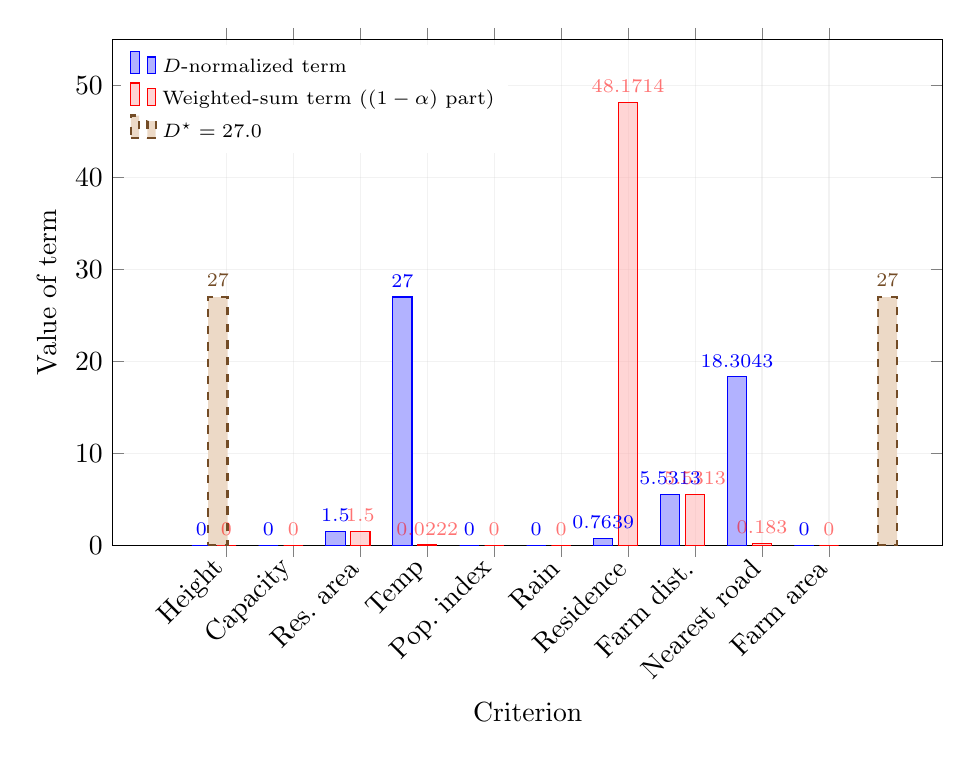
\begin{tikzpicture}
\begin{axis}[
    ybar,
    width=\textwidth,
    height=8cm,
    ymin=0,
    ymax=55, % accommodates the large p7/0.35 bar
    bar width=7pt,
    enlarge x limits=0.12,
    xlabel={Criterion},
    ylabel={Value of term},
    xtick=data,
    xticklabel style={rotate=45, anchor=east},
    xticklabels={
      Height,
      Capacity,
      Res.~area,
      Temp,
      Pop.~index,
      Rain,
      Residence,
      Farm~dist.,
      Nearest~road,
      Farm~area
    },
    legend style={draw=none, at={(0.01,0.99)}, anchor=north west, font=\scriptsize},
    legend cell align={left},
    nodes near coords,
    nodes near coords align={vertical},
    every node near coord/.append style={font=\scriptsize, /pgf/number format/fixed, /pgf/number format/precision=4},
    grid=both,
    grid style={opacity=0.2}
]
% --- Series 1: D-normalized terms (from the D-constraints) ---
% n1/47=0, n2/3=0, p3/0.04=1.5, p4/0.04=27.0, n5/48.74=0, n6/0.52=0,
% p7/22.07≈0.7639, p8/0.32=5.5313, p9/0.23≈18.3043, n10/0.68=0
\addplot+[fill] coordinates {
 (1,0.0000) (2,0.0000) (3,1.5000) (4,27.0000) (5,0.0000)
 (6,0.0000) (7,0.7639) (8,5.5313) (9,18.3043) (10,0.0000)
};
\addlegendentry{$D$-normalized term}

% --- Series 2: (1-$\alpha$) weighted-sum terms in the EGP objective ---
% Only present for p3, p4, p7, p8, p9 (others are zero here)
% p3/0.04=1.5, p4/48.74≈0.0222, p7/0.35≈48.1714, p8/0.32=5.5313, p9/23≈0.1830
\addplot+[fill, fill opacity=0.55] coordinates {
 (1,0.0000) (2,0.0000) (3,1.5000) (4,0.0222) (5,0.0000)
 (6,0.0000) (7,48.1714) (8,5.5313) (9,0.1830) (10,0.0000)
};
\addlegendentry{Weighted-sum term ($(1-\alpha)$ part)}

% Reference line at D*
\addplot+[domain=0.5:10.5, samples=2, thick, dashed] {27.0};
\addlegendentry{$D^{\star}=27.0$}
\end{axis}
\end{tikzpicture}
\caption{EGP contributions by criterion: comparison of the $D$-normalized terms (used in the minimax bound) versus the terms entering the $(1-\alpha)$ weighted-sum portion of the objective ($\alpha=0.8$). The $D$-binding criterion is \emph{Temperature}; the weighted-sum is dominated by \emph{Residence}.}
\label{fig:egpDeviations}
\end{figure}


\subsection{Lexicographic Goal Programming Solution}
In the Lexicographic Goal Programming (LGP) solution, we optimize three priority levels in sequence. \textbf{Priority~1} minimizes $(1/47)n_1+(1/3)n_2+(1/0.52)n_5+(1/0.68)n_{10}$ and attains $0$, implying no underachievement on height, capacity, population, or farmland area at the optimum. \textbf{Priority~2} then minimizes $(1/0.04)p_3+(1/48.74)p_4+(1/22.07)n_6$ subject to Priority~1’s optimum, yielding $0.0416$ (driven by temperature: $p_4/48.74\approx 0.0416$). \textbf{Priority~3} finally minimizes $(1/0.35)p_7+(1/0.32)p_8+(1/23)p_9$ under the earlier priorities, giving $83.4264$. The resulting portfolio selects Dams~\textbf{19, 21, 28} with total cost $\$158.7+\$164.3+\$172.1=\$495.1$\,M (within the \$500\,M cap). Table~\ref{tab:model_results} lists the attributes of the selected dams, and Table~\ref{tab:lgpAchievementVsTarget} reports achieved values versus targets and deviations; notably, temperature and the Priority~3 social–access criteria (residence, farmland distance, road proximity) drive the lexicographic refinement Figure \ref{fig:lgpPriorityThree}.

% =========================
% Table: lgpAchievementVsTarget
% =========================
\begin{table}[htbp]
\centering
\caption{LGP: goal achievement vs.\ targets and deviations (final portfolio; $n_i=0$)}
\label{tab:lgpAchievementVsTarget}
\begin{tabular}{clcccc}
\hline
\textbf{\#} & \textbf{Criterion} & \textbf{Target} & \textbf{Achieved} & \textbf{Deviation type} & \textbf{Value} \\
\hline
1  & Dam height (m)              & 47.00  & 123.00 & $p_{1}$  & 76.00 \\
2  & Capacity (Mm$^{3}$)         & 3.00   & 10.50  & $p_{2}$  & 7.50  \\
3  & Reservoir area (km$^{2}$)   & 0.04   & 0.04   & $p_{3}$  & 0.00  \\
4  & Temperature ($^{\circ}$C)    & 48.74  & 50.77  & $p_{4}$  & 2.03  \\
5  & Population index            & 0.52   & 1.13   & $p_{5}$  & 0.61  \\
6  & Rainfall                    & 22.07  & 55.60  & $p_{6}$  & 33.53 \\
7  & Residence                   & 1.86   & 26.02  & $p_{7}$  & 24.16 \\
8  & Farmland distance           & 0.32   & 4.80   & $p_{8}$  & 4.48  \\
9  & Nearest road                & 0.23   & 9.38   & $p_{9}$  & 9.15  \\
10 & Farmland area               & 0.68   & 36.41  & $p_{10}$ & 35.73 \\
\hline
\end{tabular}
\end{table}

% =========================
% Table: LGP priority objectives (tiny summary)
% =========================
\begin{table}[htbp]
\centering
\caption{Lexicographic GP: summary of priority objective values (final portfolio)}
\label{tab:lgpPriorityObjectives}
\begin{tabular}{clc}
\hline
\textbf{Priority} & \textbf{Objective minimized} & \textbf{Optimal value} \\
\hline
1 & $\frac{1}{47}n_1+\frac{1}{3}n_2+\frac{1}{0.52}n_5+\frac{1}{0.68}n_{10}$ & $0.0000$ \\
2 & $\frac{1}{0.04}p_3+\frac{1}{48.74}p_4+\frac{1}{22.07}n_6$               & $0.0416$ \\
3 & $\frac{1}{0.35}p_7+\frac{1}{0.32}p_8+\frac{1}{23}p_9$                    & $83.4264$ \\
\hline
\end{tabular}
\end{table}

% =========================
% Figure: Priority-3 terms bar chart
% =========================
% Preamble needs:
% \usepackage{pgfplots}
% \pgfplotsset{compat=1.18}
\begin{figure}[htbp]
\centering
\begin{tikzpicture}
\begin{axis}[
    ybar,
    width=\textwidth,
    height=7cm,
    ymin=0,
    ymax=75,
    bar width=12pt,
    enlarge x limits=0.2,
    xlabel={Priority 3 criteria},
    ylabel={Term value in objective},
    xtick=data,
    xticklabels={
      Residence $\big(\tfrac{1}{0.35}p_7\big)$,
      Farm dist. $\big(\tfrac{1}{0.32}p_8\big)$,
      Nearest road $\big(\tfrac{1}{23}p_9\big)$
    },
    nodes near coords,
    nodes near coords align={vertical},
    every node near coord/.append style={font=\scriptsize, /pgf/number format/fixed, /pgf/number format/precision=4},
    grid=both,
    grid style={opacity=0.2},
    legend style={draw=none, at={(0.02,0.98)}, anchor=north west, font=\scriptsize}
]
% Priority-3 weighted terms: p7/0.35, p8/0.32, p9/23
\addplot+[fill] coordinates {
 (1,69.0286) (2,14.0000) (3,0.3978)
};
\addlegendentry{Weighted term}

% (Optional) reference line at the total Priority-3 objective
\addplot+[domain=0.5:3.5, samples=2, thick, dashed] {83.4264};
\addlegendentry{Total $=83.4264$}

\end{axis}
\end{tikzpicture}
\caption{Lexicographic GP, Priority 3 objective components for the final portfolio: $\frac{1}{0.35}p_7=69.0286$, $\frac{1}{0.32}p_8=14.0000$, and $\frac{1}{23}p_9=0.3978$. Their sum equals the Priority 3 value $83.4264$.}
\label{fig:lgpPriorityThree}
\end{figure}


In Fig.~\ref{fig:lgpPriorityThree}, a clear pattern emerges. \textbf{Dam\~19} is selected by all four models, indicating a robust choice insensitive to the change from weighted-sum (WGP) to Chebyshev (CGP) to extended (EGP) and lexicographic (LGP) formulations. A near-core site, \textbf{Dam\~28}, appears in three models (CGP, EGP, LGP) but not WGP, suggesting that minimax and priority-based emphases favor it. The remaining slot is model-sensitive: WGP picks {18, 23}, CGP swaps in {20}, EGP prefers {16}, and LGP chooses {21}. Overall, moving from WGP to CGP/EGP/LGP consolidates consensus around {19, 28} while the third selection pivots according to each model’s treatment of deviations (weighted-sum vs.\ max-deviation vs.\ lexicographic priorities).

% Requires in preamble:
% \usepackage{pgfplots}
% \pgfplotsset{compat=1.18}

\begin{figure}[htbp]
\centering
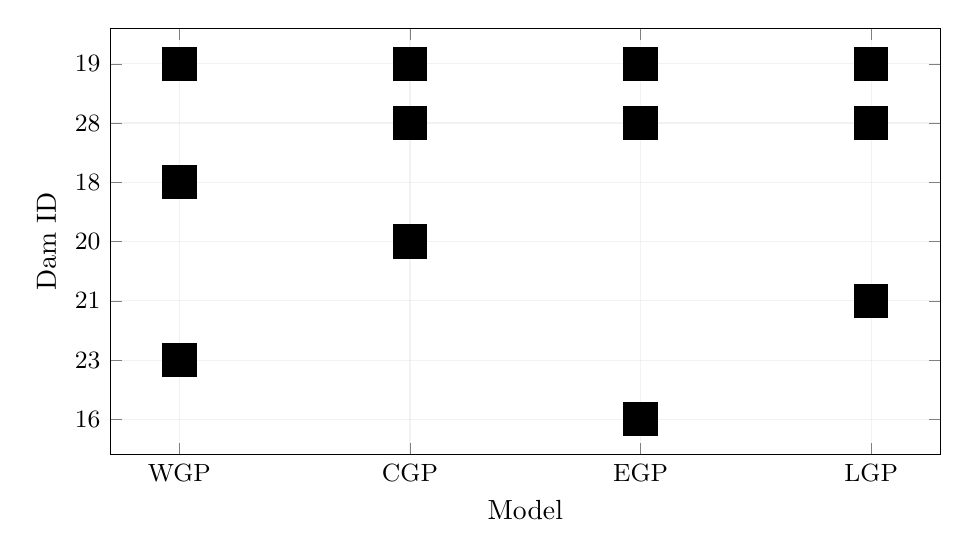
\begin{tikzpicture}
\begin{axis}[
  width=\textwidth,
  height=7cm,
  xlabel={Model},
  ylabel={Dam ID},
  xtick=data,
  ytick=data,
  symbolic x coords={WGP,CGP,EGP,LGP},
  symbolic y coords={19,28,18,20,21,23,16},
  y dir=reverse,
  grid=both,
  grid style={opacity=0.2},
  tick label style={font=\small},
]
\addplot[
  only marks,
  mark=square*,
  mark size=6pt
] coordinates {
  (WGP,19) (WGP,18) (WGP,23)
  (CGP,19) (CGP,20) (CGP,28)
  (EGP,19) (EGP,28) (EGP,16)
  (LGP,19) (LGP,28) (LGP,21)
};
\end{axis}
\end{tikzpicture}
\caption{Model–dam selection map for the four GP variants. Dam 19 is chosen by all four; Dam 28 by three (CGP, EGP, LGP); the others are singletons (WGP: 18, 23; CGP: 20; EGP: 16; LGP: 21).}
\label{fig:modelDamSelectionMap}
\end{figure}


\subsection{Multi-Choice GP Extension Solutions}
% % In preamble:
% % \usepackage{pgfplots}
% % \pgfplotsset{compat=1.18}
% \begin{figure}[htbp]
% \centering
% \begin{tikzpicture}
% \begin{axis}[
%   ybar,
%   bar width=10pt,
%   width=15cm,
%   height=8cm,
%   ymin=0,
%   ylabel={Objective function value (fval)},
%   xlabel={Model},
%   symbolic x coords={WGP,CGP,EGP,LGP-P3},
%   xtick=data,
%   enlarge x limits=0.2,
%   ymajorgrids,
%   legend style={at={(0.5,-0.18)},anchor=north,legend columns=2,font=\small},
% nodes near coords,
% nodes near coords style={rotate=45, anchor=west, font=\footnotesize},
%   every node near coord/.append style={font=\footnotesize}
% ]

% % Base models
% \addplot+[fill=gray!40, draw=gray!70]
%   coordinates {(WGP,14.9277) (CGP,25.2174) (EGP,32.6816) (LGP-P3,83.4264)};
% \addlegendentry{Base}

% % MCGP
% \addplot+[fill=blue!45, draw=blue!70]
%   coordinates {(WGP,28.7245) (CGP,25.1304) (EGP,32.5462) (LGP-P3,82.7889)};
% \addlegendentry{MCGP}

% \end{axis}
% \end{tikzpicture}
% \caption{Comparison of \textit{fval} for Base vs.\ MCGP variants across models.}
% \label{fig:fval_base_vs_mcgp}
% \end{figure}

\begin{figure}[htbp]
\centering
\begin{tikzpicture}
\begin{axis}[
  ybar,
  bar width=10pt,
  width=15cm,
  height=8cm,
  ymin=0,
  ylabel={Objective function value (fval)},
  xlabel={Model},
  symbolic x coords={WGP,CGP,EGP,LGP-P1,LGP-P2,LGP-P3},
  xtick=data,
  enlarge x limits=0.08,
  ymajorgrids,
  legend style={at={(0.5,-0.18)},anchor=north,legend columns=2,font=\small},
  nodes near coords,
  nodes near coords style={
    /pgf/number format/fixed,
    /pgf/number format/precision=2,
    font=\footnotesize,
    text=black,           % ← force value labels to black
    rotate=45, anchor=west
  },
  tick label style={font=\small},
  label style={font=\small}
]

% Base (uses \definecolor{barfillbase}{HTML}{B0A195} in preamble)
\addplot+[fill=barfillbase, draw=barfillbase!60!black]
  coordinates {
    (WGP,14.93)
    (CGP,25.28)
    (EGP,32.68)
    (LGP-P1,0)
    (LGP-P2,0.0416)
    (LGP-P3,83.46)
  };
\addlegendentry{Base}

% MCGP (uses \definecolor{barfillmcgp}{HTML}{838A94} in preamble)
\addplot+[fill=barfillmcgp, draw=barfillmcgp!60!black]
  coordinates {
    (WGP,28.7245)
    (CGP,25.1304)
    (EGP,32.5462)
    (LGP-P1,0)
    (LGP-P2,0.0416)
    (LGP-P3,82.79)
  };
\addlegendentry{MCGP}

\end{axis}
\end{tikzpicture}
\caption{Side-by-side comparison of \textit{fval} for Base vs.\ MCGP across models.}
\label{fig:fval_base_vs_mcgp}
\end{figure}

\begin{figure}[htbp]
\centering
\begin{tikzpicture}
\begin{axis}[
  title={Selected Dam Sites by Model: Base vs.\ MCGP},
  xlabel={Model / Variant},
  ylabel={Dam site ID},
  symbolic x coords={
    WGP--Base,WGP--MCGP,
    CGP--Base,CGP--MCGP,
    EGP--Base,EGP--MCGP,
    LGP-P3--Base,LGP-P3--MCGP
  },
  xtick=data,
  ymin=0, ymax=29,
  ytick={1,2,...,28},
  x tick label style={rotate=45,anchor=east,font=\small},
  width=16.5cm, height=9.5cm,
  grid=both, minor tick num=1
]

% All points same color (blue circles)
\addplot+[only marks, mark=*, mark options={fill=barfillbase, draw=barfillbase}, mark size=2.8pt]
  coordinates {
    % ---------- WGP ----------
    (WGP--Base,3) (WGP--Base,18) (WGP--Base,19)
    (WGP--MCGP,1) (WGP--MCGP,19) (WGP--MCGP,23)

    % ---------- CGP ----------
    (CGP--Base,19) (CGP--Base,20) (CGP--Base,28)
    (CGP--MCGP,19) (CGP--MCGP,20) (CGP--MCGP,28)

    % ---------- EGP ----------
    (EGP--Base,16) (EGP--Base,19) (EGP--Base,28)
    (EGP--MCGP,19) (EGP--MCGP,20) (EGP--MCGP,28)

    % ---------- LGP-P3 ----------
    (LGP-P3--Base,19) (LGP-P3--Base,21) (LGP-P3--Base,28)
    (LGP-P3--MCGP,19) (LGP-P3--MCGP,21) (LGP-P3--MCGP,28)
  };

\end{axis}
\end{tikzpicture}
\caption{Selected dam sites for each model under Base and MCGP formulations. All markers are blue circles; x-axis labels indicate the model variant.}
\label{fig:site_selection_base_vs_mcgp}
\end{figure}


\subsubsection{Weighted GP}
In the multi–choice extension of the weighted goal program (WGP–MCGP), five social/access criteria were allowed target flexibility. The model selected the lower bounds for \emph{Population} (0.52) and \emph{Farmland area} (0.68), while adopting the upper bounds for \emph{Nearest residence} (2.05), \emph{Farmland distance} (0.35), and \emph{Nearest road} (0.25), as shown in Table~\ref{tab:wgpMC_choices}. The resulting weighted deviation objective is $28.7245$, which is higher than the fixed–target WGP value ($14.9277$) by $+13.7968$ (Figure \ref{tab:wgpMCGPSummary}), reflecting the tighter upper–bound targets imposed on three criteria. Fig.~\ref{fig:wgpMC_intervals} visualizes the chosen target levels across the flexible goals and the model output is reported in \ref{tab:mcgpResult}.      

\begin{table}[htbp]
\centering
\caption{WGP–MCGP: flexible criteria, available targets, and chosen level (from $z$).}
\label{tab:wgpMC_choices}
\begin{tabular}{lccc}
\hline
\textbf{Criterion} & \textbf{Lower target (L)} & \textbf{Upper target (U)} & \textbf{Chosen} \\
\hline
Population index      & 0.52 & 0.57 & L (0.52) \\
Nearest residence     & 1.86 & 2.05 & U (2.05) \\
Farmland distance     & 0.32 & 0.35 & U (0.35) \\
Nearest road          & 0.23 & 0.25 & U (0.25) \\
Farmland area         & 0.68 & 0.75 & L (0.68) \\
\hline
\end{tabular}
\end{table}

% =========================
% Update to Table: WGP vs WGP–MCGP summary
% =========================
\begin{table}[htbp]
\centering
\caption{WGP vs.\ WGP–MCGP summary.}
\label{tab:wgpMCGPSummary}
\begin{tabular}{l l c c c}
\hline
\textbf{Model} & \textbf{Portfolio} & \textbf{Cost (M\$)} & \textbf{Objective} & \(\Delta\) vs.\ WGP \\
\hline
WGP (fixed targets)   & \{18,19,23\} & 481.5 & 14.9277 & -- \\
WGP–MCGP (flexible)   & \{1,19,23\}  & 487.4 & 28.7245 & +13.7968 \\
\hline
\end{tabular}
\end{table}

% Preamble: \usepackage{pgfplots} \pgfplotsset{compat=1.18}
\begin{figure}[htbp]
\centering
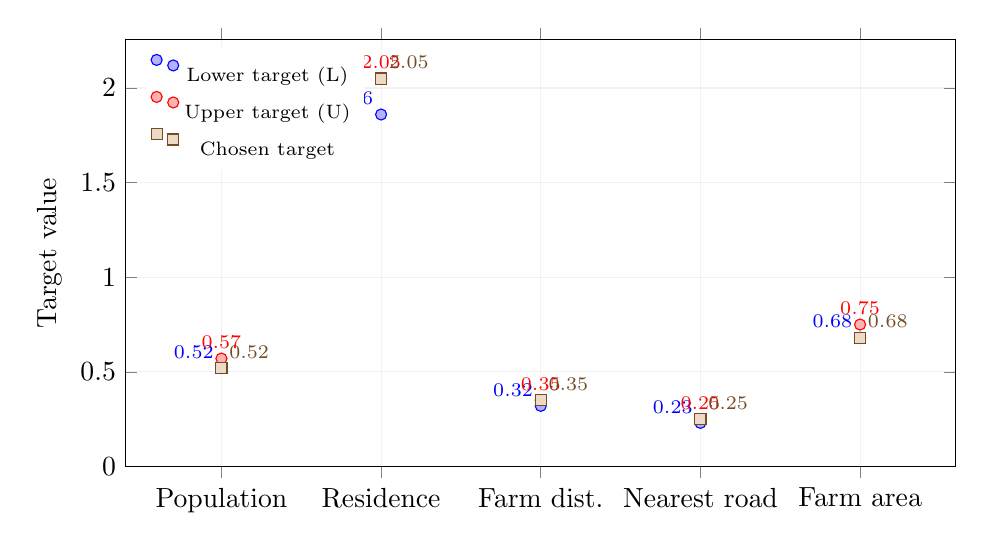
\begin{tikzpicture}
\begin{axis}[
  ybar=0pt,
  width=\textwidth, height=7cm,
  xtick=data,
  xticklabels={Population, Residence, Farm dist., Nearest road, Farm area},
  ylabel={Target value},
  ymin=0, enlarge x limits=0.15,
  grid=both, grid style={opacity=0.2},
  legend style={draw=none, at={(0.02,0.98)}, anchor=north west, font=\scriptsize},
  nodes near coords, nodes near coords align={vertical},
  every node near coord/.append style={font=\scriptsize}
]
% Lower targets (L)
\addplot+[mark=*, only marks] coordinates {(1,0.52) (2,1.86) (3,0.32) (4,0.23) (5,0.68)};
\addlegendentry{Lower target (L)}

% Upper targets (U)
\addplot+[mark=*, only marks] coordinates {(1,0.57) (2,2.05) (3,0.35) (4,0.25) (5,0.75)};
\addlegendentry{Upper target (U)}

% Chosen targets (from z) — plotted slightly above with square markers
\addplot+[mark=square*, only marks] coordinates {(1,0.52) (2,2.05) (3,0.35) (4,0.25) (5,0.68)};
\addlegendentry{Chosen target}
\end{axis}
\end{tikzpicture}
\caption{WGP–MCGP target flexibility across five criteria: chosen levels (squares) relative to the available lower/upper targets (dots).}
\label{fig:wgpMC_intervals}
\end{figure}


\subsubsection{Chebyshev GP}
Allowing target flexibility on five socio-environmental criteria retains the CGP portfolio $\{19,20,28\}$ while slightly improving the minimax objective from $D^{\star}\!=\!25.2174$ to $25.1304$ (Table~\ref{tab:cgpMCGPSummary}). The model chooses the lower targets for Population and Farmland area, and the upper targets for Nearest residence, Farmland distance, and Nearest road (Table~\ref{tab:cgpMCGPTargets}). With the selected dams, the worst normalized deviation is still \emph{Nearest road} ($p_9/0.23$), followed by Farmland distance and Reservoir area (Figure~\ref{fig:cgpMCGPDeviations}); all other normalized deviations are zero in the minimax sense. Achieved values relative to the chosen targets are detailed in Table~\ref{tab:cgpMCGPAchievementVsTarget} and the model output is reported in \ref{tab:mcgpResult}

% =========================
% CGP–MCGP: summary vs base CGP
% =========================
\begin{table}[htbp]
\centering
\caption{Chebyshev GP (CGP) vs. CGP–MCGP with target flexibility on five goals.}
\label{tab:cgpMCGPSummary}
\begin{tabular}{lcccc}
\toprule
Model & Selected dams & Total cost (M\$) & $D^\star$ & $\Delta D$ vs. CGP \\
\midrule
CGP (fixed targets)   & \{19, 20, 28\} & 497.3 & 25.2174 & -- \\
CGP--MCGP (flexible)  & \{19, 20, 28\} & 497.3 & 25.1304 & $-0.0870$ (–0.345\%) \\
\bottomrule
\end{tabular}
\end{table}
% =========================
% CGP–MCGP: chosen target levels (z)
% =========================
\begin{table}[htbp]
\centering
\caption{CGP--MCGP chosen targets for flexible goals (binary $z_k$: 1 = lower target, 0 = upper target).}
\label{tab:cgpMCGPTargets}
\begin{tabular}{llll}
\toprule
Criterion & Target options & Chosen ($z_k$) & Target used \\
\midrule
Population                 & $0.52$ (low) \;|\; $0.57$ (high) & $z_1=1$ & $0.52$ \\
Nearest residence          & $1.86$ (low) \;|\; $2.05$ (high) & $z_2=0$ & $2.05$ \\
Farmland distance          & $0.32$ (low) \;|\; $0.35$ (high) & $z_3=0$ & $0.35$ \\
Nearest road               & $0.23$ (low) \;|\; $0.25$ (high) & $z_4=0$ & $0.25$ \\
Farmland area              & $0.68$ (low) \;|\; $0.75$ (high) & $z_5=1$ & $0.68$ \\
\bottomrule
\end{tabular}
\end{table}
% =========================
% Figure: cgpMC_deviations (normalized terms entering D)
% =========================
% Preamble needs:
% \usepackage{pgfplots}
% \pgfplotsset{compat=1.18}
\begin{figure}[htbp]
\centering
\begin{tikzpicture}
\begin{axis}[
    ybar,
    width=\textwidth,
    height=7cm,
    ymin=0,
    bar width=8pt,
    enlarge x limits=0.08,
    xlabel={Criterion (normalized term in $D$)},
    ylabel={Weighted deviation},
    xtick=data,
    xticklabel style={rotate=45, anchor=east},
    xticklabels={
      Height $(\tfrac{1}{47}n_1)$,
      Capacity $(\tfrac{1}{3}n_2)$,
      Res.~area $(\tfrac{1}{0.04}p_3)$,
      Temp $(\tfrac{1}{0.04}p_4)$,
      Pop. $(\tfrac{1}{48.74}n_5)$,
      Rain $(\tfrac{1}{0.52}n_6)$,
      Residence $(\tfrac{1}{22.07}p_7)$,
      Farm dist. $(\tfrac{1}{0.32}p_8)$,
      Nearest road $(\tfrac{1}{0.23}p_9)$,
      Farm area $(\tfrac{1}{0.68}n_{10})$
    },
    nodes near coords,
    nodes near coords align={vertical},
    every node near coord/.append style={font=\scriptsize, /pgf/number format/precision=4, /pgf/number format/fixed},
    grid=both,
    grid style={opacity=0.2},
    legend style={at={(0.02,0.98)},anchor=north west,draw=none,fill=none}
]
% Normalized deviations entering D:
% n1=0, n2=0, p3/0.04=10.5, p4/0.04=0, n5=0, n6=0, p7/22.07≈0.6203, p8/0.32=12.3438, p9/0.23=25.1304, n10=0
\addplot coordinates {
 (1,0.0000) (2,0.0000) (3,10.5000) (4,0.0000) (5,0.0000)
 (6,0.0000) (7,0.6203) (8,12.3438) (9,25.1304) (10,0.0000)
};
% Draw D* as a reference line
\addplot+[domain=0.5:10.5, samples=2] {25.1304};
\addlegendentry{$D^{\star}=25.1304$}
\end{axis}
\end{tikzpicture}
\caption{CGP--MCGP normalized deviations in the minimax objective. The binding criterion remains \emph{Nearest road} with $p_9/0.23=D^{\star}$; flexibility slightly reduces the worst normalized deviation compared to fixed-target CGP.}
\label{fig:cgpMCGPDeviations}
\end{figure}

% =========================
% CGP–MCGP: goal achievement vs. chosen target
% =========================
\begin{table}[htbp]
\centering
\caption{CGP--MCGP achievements vs. (chosen) targets and deviations for the selected set $\{19,20,28\}$.}
\label{tab:cgpMCGPAchievementVsTarget}
\begin{tabular}{llrrl}
\toprule
\# & Criterion & Target & Achieved & Deviation \\
\midrule
1  & Height (m)                   & 47.00  & 138.00 & $p_1=91.00$ \\
2  & Capacity (Mm$^3$)            & 3.00   & 71.50  & $p_2=68.50$ \\
3  & Reservoir area (km$^2$)      & 0.04   & 0.46   & $p_3=0.42$ \\
4  & Temperature ($^{\circ}$C)    & 48.74  & 48.74  & $p_4=0.00$ \\
5  & Population (0--50, norm.)    & 0.52   & 2.09   & $p_5=1.57$ \\
6  & Rainfall (cm)                & 22.07  & 63.76  & $p_6=41.69$ \\
7  & Nearest residence (km)       & 2.05   & 15.74  & $p_7=13.69$ \\
8  & Farmland distance (km)       & 0.35   & 4.30   & $p_8=3.95$ \\
9  & Nearest road (km)            & 0.25   & 6.03   & $p_9=5.78$ \\
10 & Farmland area (km$^2$)       & 0.68   & 24.71  & $p_{10}=24.03$ \\
\bottomrule
\end{tabular}
\end{table} 

\subsubsection{Extended GP}
With $\alpha=0.8$, the extended goal program under multi-choice targets selects the same portfolio as the CGP--MCGP case, $\{19,20,28\}$, at a total cost of \$497.3\,M (Table~\ref{tab:egpMCGPSummary}). Target flexibility is exercised by choosing lower bounds for Population and Farmland area and upper bounds for Nearest residence, Farmland distance, and Nearest road (Table~\ref{tab:egpMCGPTargets}). The worst normalized deviation remains \emph{Nearest road} ($p_9/0.23=25.1304$), defining $D^{\star}$, followed by Farmland distance and Reservoir area (Figure~\ref{fig:egpMCGPDeviations}). The composite objective evaluates to $f=0.8\times 25.1304 + 0.2\times 62.2094 = 32.5462$, indicating that the portfolio balances a modest improvement in the minimax term with a larger weighted-sum contribution, consistent with the $\alpha$-weighted trade-off; per-criterion achievements and deviations are listed in Table~\ref{tab:egpMCGPAchievementVsTarget}.


% =========================
% EGP–MCGP: summary
% =========================
\begin{table}[htbp]
\centering
\caption{Extended Goal Programming with Multi-Choice targets (EGP--MCGP), $\alpha=0.8$.}
\label{tab:egpMCGPSummary}
\begin{tabular}{lccccc}
\toprule
Model & Selected dams & Total cost (M\$) & $D^{\star}$ & WGP term $S$ & Objective $f=\alpha D+(1-\alpha)S$\\
\midrule
EGP--MCGP & \{19, 20, 28\} & 497.3 & 25.1304 & 62.2094 & 32.5462 \\
\bottomrule
\end{tabular}
\end{table}


% =========================
% EGP–MCGP: chosen target levels (z)
% =========================
\begin{table}[htbp]
\centering
\caption{EGP--MCGP chosen targets for flexible goals (binary $z_k$: 1 = lower target, 0 = upper target).}
\label{tab:egpMCGPTargets}
\begin{tabular}{llll}
\toprule
Criterion & Target options & Chosen ($z_k$) & Target used \\
\midrule
Population                 & $0.52$ (low) \;|\; $0.57$ (high) & $z_1=1$ & $0.52$ \\
Nearest residence          & $1.86$ (low) \;|\; $2.05$ (high) & $z_2=0$ & $2.05$ \\
Farmland distance          & $0.32$ (low) \;|\; $0.35$ (high) & $z_3=0$ & $0.35$ \\
Nearest road               & $0.23$ (low) \;|\; $0.25$ (high) & $z_4=0$ & $0.25$ \\
Farmland area              & $0.68$ (low) \;|\; $0.75$ (high) & $z_5=1$ & $0.68$ \\
\bottomrule
\end{tabular}
\end{table}
% =========================
% EGP–MCGP: goal achievement vs. chosen target
% =========================
\begin{table}[htbp]
\centering
\caption{EGP--MCGP achievements vs. (chosen) targets and deviations for the selected set $\{19,20,28\}$.}
\label{tab:egpMCGPAchievementVsTarget}
\begin{tabular}{llrrl}
\toprule
\# & Criterion & Target & Achieved & Deviation \\
\midrule
1  & Height (m)                   & 47.00  & 138.00 & $p_1=91.00$ \\
2  & Capacity (Mm$^3$)            & 3.00   & 71.50  & $p_2=68.50$ \\
3  & Reservoir area (km$^2$)      & 0.04   & 0.46   & $p_3=0.42$ \\
4  & Temperature ($^{\circ}$C)    & 48.74  & 48.74  & $p_4=0.00$ \\
5  & Population (0--50, norm.)    & 0.52   & 2.09   & $p_5=1.57$ \\
6  & Rainfall (cm)                & 22.07  & 63.76  & $p_6=41.69$ \\
7  & Nearest residence (km)       & 2.05   & 15.74  & $p_7=13.69$ \\
8  & Farmland distance (km)       & 0.35   & 4.30   & $p_8=3.95$ \\
9  & Nearest road (km)            & 0.25   & 6.03   & $p_9=5.78$ \\
10 & Farmland area (km$^2$)       & 0.68   & 24.71  & $p_{10}=24.03$ \\
\bottomrule
\end{tabular}
\end{table}
% =========================
% Figure: egpMC_deviations (normalized terms entering D)
% =========================
% Preamble needs:
% \usepackage{pgfplots}
% \pgfplotsset{compat=1.18}
\begin{figure}[htbp]
\centering
\begin{tikzpicture}
\begin{axis}[
    ybar,
    width=\textwidth,
    height=7cm,
    ymin=0,
    bar width=8pt,
    enlarge x limits=0.08,
    xlabel={Criterion (normalized term in $D$)},
    ylabel={Weighted deviation},
    xtick=data,
    xticklabel style={rotate=45, anchor=east},
    xticklabels={
      Height $(\tfrac{1}{47}n_1)$,
      Capacity $(\tfrac{1}{3}n_2)$,
      Res.~area $(\tfrac{1}{0.04}p_3)$,
      Temp $(\tfrac{1}{0.04}p_4)$,
      Pop. $(\tfrac{1}{48.74}n_5)$,
      Rain $(\tfrac{1}{0.52}n_6)$,
      Residence $(\tfrac{1}{22.07}p_7)$,
      Farm dist. $(\tfrac{1}{0.32}p_8)$,
      Nearest road $(\tfrac{1}{0.23}p_9)$,
      Farm area $(\tfrac{1}{0.68}n_{10})$
    },
    nodes near coords,
    nodes near coords align={vertical},
    every node near coord/.append style={font=\scriptsize, /pgf/number format/precision=4, /pgf/number format/fixed},
    grid=both,
    grid style={opacity=0.2},
    legend style={at={(0.02,0.98)},anchor=north west,draw=none,fill=none}
]
% Normalized deviations entering D:
% n1=0, n2=0, p3/0.04=10.5, p4/0.04=0, n5=0, n6=0, p7/22.07≈0.6203, p8/0.32=12.3438, p9/0.23=25.1304, n10=0
\addplot coordinates {
 (1,0.0000) (2,0.0000) (3,10.5000) (4,0.0000) (5,0.0000)
 (6,0.0000) (7,0.6203) (8,12.3438) (9,25.1304) (10,0.0000)
};
% Draw D* as a reference line
\addplot+[domain=0.5:10.5, samples=2] {25.1304};
\addlegendentry{$D^{\star}=25.1304$}
\end{axis}
\end{tikzpicture}
\caption{EGP--MCGP normalized deviations in the minimax term $D$. The binding criterion is \emph{Nearest road} with $p_9/0.23=D^{\star}$; next are Farmland distance and Reservoir area.}
\label{fig:egpMCGPDeviations}
\end{figure}

\subsubsection{Lexicographic GP}
Relative to the baseline LGP, introducing multi-choice targets leaves the Priority~1 and Priority~2 objectives unchanged while delivering a modest improvement at Priority~3 (from 83.4264 to 82.7889; Table~\ref{tab:LGPVsLGPMCObjectives}, Fig.~\ref{fig:LGPVsLGPMCObjectives}). The chosen target pattern is consistent across priorities—lower targets for Population and Farmland area, upper targets for Nearest residence, Farmland distance, and Nearest road (Table~\ref{tab:LPGMCGPTargets})—and the P1 portfolio is \{\LGPMCselPone\}, with the final P3 portfolio shown in Table~\ref{tab:LGP_LGPMC_selected_sets} and Fig. \ref{fig:lgpmc_selection_map}.


% =============================
% FIGURE 1: Objective comparison by priority
% =============================
\begin{figure}[htbp]
\centering
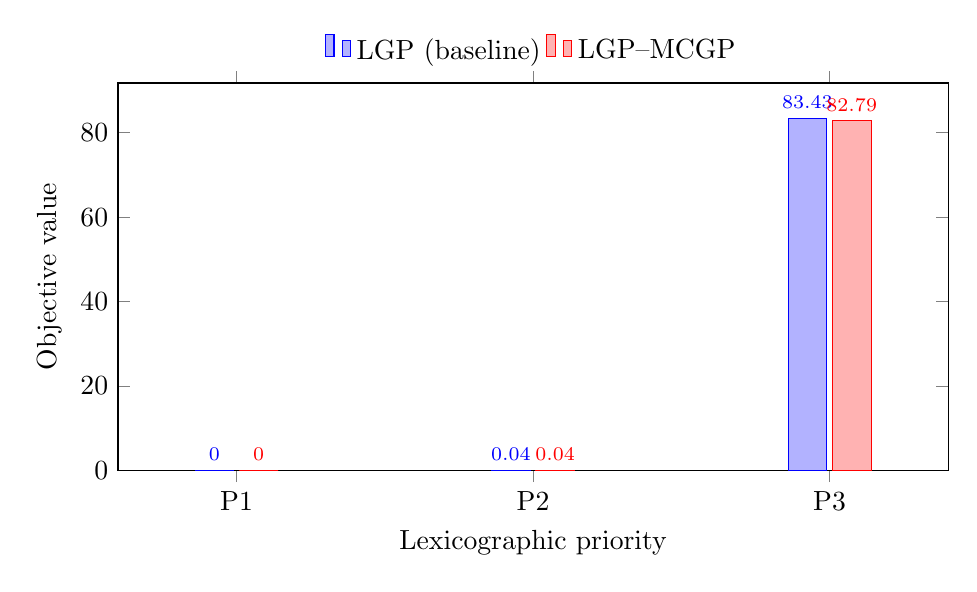
\begin{tikzpicture}
\begin{axis}[
  ybar,
  width=\textwidth, height=6.5cm,
  bar width=14pt,
  ymin=0,
  enlarge x limits=0.20,
  ylabel={Objective value},
  xlabel={Lexicographic priority},
  symbolic x coords={P1,P2,P3},
  xtick=data,
  legend style={at={(0.5,1.02)},anchor=south,legend columns=-1,draw=none,fill=none},
  nodes near coords,
  every node near coord/.append style={font=\scriptsize,/pgf/number format/fixed}
]
\addplot coordinates {(P1,\LGPpOne) (P2,\LGPpTwo) (P3,\LGPpThree)};
\addplot coordinates {(P1,\LGPMCpOne) (P2,\LGPMCpTwo) (P3,\LGPMCpThree)};
\legend{LGP (baseline), LGP--MCGP}
\end{axis}
\end{tikzpicture}
\caption{Lexicographic objectives by priority. MCGP matches P1 and P2 and achieves a small improvement at P3 ($\approx0.64$).}
\label{fig:LGPVsLGPMCObjectives}
\end{figure}
% =============================
% TABLE 2: MCGP target choices (z) and used targets
% =============================
\begin{table}[htbp]
\centering
\caption{LGP--MCGP target flexibility (binary $z_k$: 1 = lower target, 0 = upper target).}
\label{tab:LPGMCGPTargets}
\begin{tabular}{llll}
\toprule
Criterion & Options & $z_k$ & Target used \\
\midrule
Population            & $0.52$ (low) \;|\; $0.57$ (high) & \zPop   & $0.52$ \\
Nearest residence (km)& $1.86$ (low) \;|\; $2.05$ (high) & \zRes   & $2.05$ \\
Farmland distance (km)& $0.32$ (low) \;|\; $0.35$ (high) & \zFarmD & $0.35$ \\
Nearest road (km)     & $0.23$ (low) \;|\; $0.25$ (high) & \zRoad  & $0.25$ \\
Farmland area (km$^2$)& $0.68$ (low) \;|\; $0.75$ (high) & \zFarmA & $0.68$ \\
\bottomrule
\end{tabular}
\end{table}
% =============================
% TABLE 3: Selected dam sets (IDs)
% =============================
\begin{table}[htbp]
\centering
\caption{Selected dam IDs across priorities.}
\label{tab:LGP_LGPMC_selected_sets}
\begin{tabular}{lll}
\toprule
Case & Priority & Selected dams (IDs) \\
\midrule
LGP (baseline)   & Final & \{\LGPbaseSel\} \\
LGP--MCGP        & P1    & \{\LGPMCselPone\} \\
LGP--MCGP        & P2    & \{\LGPMCselPtwo\} \\
LGP--MCGP        & P3    & \{\LGPMCselPthree\} \\
\bottomrule
\end{tabular}
\end{table}
% =============================
% FIGURE 1: Objective comparison by priority
% =============================
\begin{figure}[htbp]
\centering
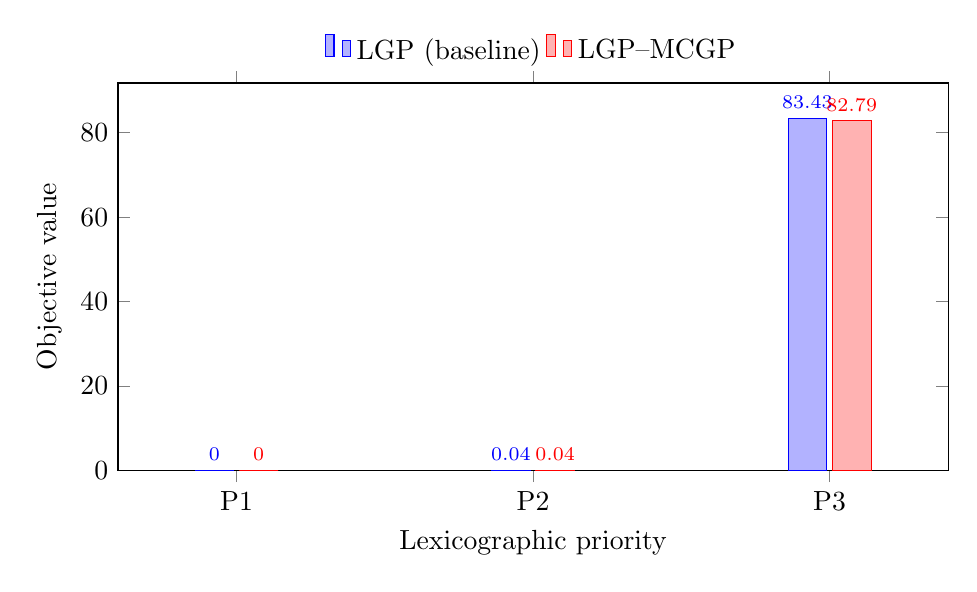
\begin{tikzpicture}
\begin{axis}[
  ybar,
  width=\textwidth, height=6.5cm,
  bar width=14pt,
  ymin=0,
  enlarge x limits=0.20,
  ylabel={Objective value},
  xlabel={Lexicographic priority},
  symbolic x coords={P1,P2,P3},
  xtick=data,
  legend style={at={(0.5,1.02)},anchor=south,legend columns=-1,draw=none,fill=none},
  nodes near coords,
  every node near coord/.append style={font=\scriptsize,/pgf/number format/fixed}
]
\addplot coordinates {(P1,\LGPpOne) (P2,\LGPpTwo) (P3,\LGPpThree)};
\addplot coordinates {(P1,\LGPMCpOne) (P2,\LGPMCpTwo) (P3,\LGPMCpThree)};
\legend{LGP (baseline), LGP--MCGP}
\end{axis}
\end{tikzpicture}
\caption{Lexicographic objectives by priority. MCGP matches P1 and P2 and achieves a small improvement at P3 ($\approx0.64$).}
\label{fig:LGPVsLGPMCObjectives}
\end{figure}
% =============================
% FIGURE: Selection map across priorities (no macros, fully explicit)
% Needs: \usepackage{pgfplots} \pgfplotsset{compat=1.18}
% =============================
\begin{figure}[htbp]
\centering
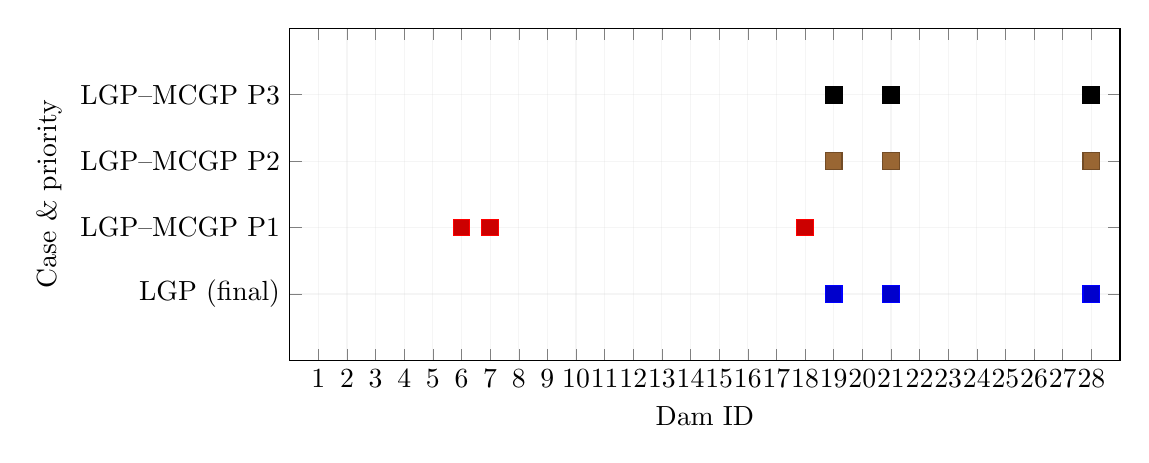
\begin{tikzpicture}
\begin{axis}[
  width=\textwidth, height=5.8cm,
  xmin=0, xmax=29, ymin=0, ymax=5, % integers -> robust parsing
  xlabel={Dam ID}, ylabel={Case \& priority},
  ytick={1,2,3,4},
  yticklabels={LGP (final), LGP--MCGP P1, LGP--MCGP P2, LGP--MCGP P3},
  xtick={1,2,...,28},
  grid=both, grid style={opacity=0.15},
  enlargelimits=false,
]

% Row 1: LGP (final) -> {19,21,28}
\addplot+[only marks,mark=square*,mark size=3pt]
  coordinates {(19,1) (21,1) (28,1)};

% Row 2: LGP–MCGP P1 -> {6,7,18}
\addplot+[only marks,mark=square*,mark size=3pt]
  coordinates {(6,2) (7,2) (18,2)};

% Row 3: LGP–MCGP P2 -> {19,21,28}
\addplot+[only marks,mark=square*,mark size=3pt]
  coordinates {(19,3) (21,3) (28,3)};

% Row 4: LGP–MCGP P3 -> {19,21,28}
\addplot+[only marks,mark=square*,mark size=3pt]
  coordinates {(19,4) (21,4) (28,4)};

\end{axis}
\end{tikzpicture}
\caption{Selected-dam map across LGP baseline and LGP–MCGP priorities. Filled squares mark dams included in each portfolio.}
\label{fig:lgpmc_selection_map}
\end{figure}



\subsection{Sensitivity Analysis}
Sensitivity analysis (SA) is a crucial step in multi-criteria decision-making (MCDM), as it evaluates the robustness of solutions when key model parameters are perturbed. In goal programming applications, where weights, targets, and other constraints guide the optimization, small changes can sometimes lead to disproportionately large shifts in the selected alternatives or in the overall objective performance. Testing models under these conditions therefore helps answer the central question: are the solutions stable enough to be trusted for real-world implementation, or do they fluctuate under modest changes in assumptions?

In this study, two types of sensitivity analysis were carried out to systematically investigate robustness across the four goal programming models considered—Weighted Goal Programming (WGP), Lexicographic Goal Programming (LGP), Chebyshev Goal Programming (CGP), and Extended Goal Programming (EGP).

We varied the distribution of weights across objectives using ten randomized test sets and compared the resulting solutions against the base model. The purpose was to determine whether changes in emphasis among objectives significantly alter the selection of dam sites or the associated objective function values. Key questions included: Which dam sites are consistently selected across different weight configurations? Which sites appear only under specific weight emphases? How variable are the objective values under weight perturbations?

Here, the emphasis shifted from weights to the target levels defined for each goal. Ten different target scenarios were generated and applied across all four models, with results compared against their respective base solutions. The objective was to assess: How sensitive is each model to adjustments in target values? Do some models show large swings in objective values while others remain stable? Which dam sites persistently appear across target variations, and which are target-sensitive?

Together, these analyses offer complementary insights. Weight SA reveals the impact of subjective trade-offs among competing objectives, while Target SA shows how solution stability depends on the feasibility and realism of the goals themselves. In the following sections, we first present the results of Weight SA, before moving on to Target SA.

\subsubsection{Weight Analysis}
The weight sensitivity analysis focused on how variations in the relative importance of objectives influenced the Weighted Goal Programming (WGP) and Lexicographic Goal Programming (LGP) models. Figure \ref{fig:weight_heatmap} maps dam-site selections across ten randomized weight sets compared with the base WGP solution. The heatmap shows that dams 18 and 19 were consistently chosen in nearly all scenarios, while other sites such as 12, 13, and 23 appeared only under specific weight allocations. This highlights the presence of a “core set” of robust sites that are insensitive to weight perturbations, alongside more marginal sites that enter solutions when emphasis shifts to particular objectives.

Objective function values also varied under weight perturbations. The lollipop plot in Figure \ref{fig:wgp_sa_lollipop_fval} compares the performance of each test set against the base WGP solution. While the base solution achieved an objective value of 14.93, the sensitivity runs produced substantially lower values ranging between 0.26 and 2.50. This suggests that, although the base configuration is balanced across objectives, certain weight allocations heavily prioritize specific goals at the expense of overall balance, yielding smaller numerical deviations. In other words, the weight distribution strongly shapes model efficiency, but the solutions remain internally consistent across scenarios.

A more direct measure of robustness is shown in the frequency analysis of dam selections (Figure \ref{fig:wgp_sa_frequency}). Dam 18 was selected in 70\% of runs, dam 19 in 80\%, and dam 23 in 60\%, while other sites appeared much less frequently. The overlay of the base solution confirms that the sites chosen there align with those most frequently selected under sensitivity runs, reinforcing the interpretation of robustness. Finally, the LGP model illustrates a different dynamic (Figure \ref{fig:lgp_fval_tradeoff}): while Priority 1 and Priority 2 objectives remain essentially stable across weight sets, Priority 3 shows wide variation, with objective values ranging from 2.5 to 13.1. This reflects the lexicographic structure—higher priorities dominate decision outcomes, leaving lower priorities sensitive to residual trade-offs. Together, these findings show that weight changes mainly affect the inclusion of marginal dam sites and the performance of lower-priority goals, while a stable subset of core sites persists across scenarios.

% Requires in preamble:
% \usepackage{pgfplots}
% \pgfplotsset{compat=1.18}

\begin{figure}[htbp]
\centering
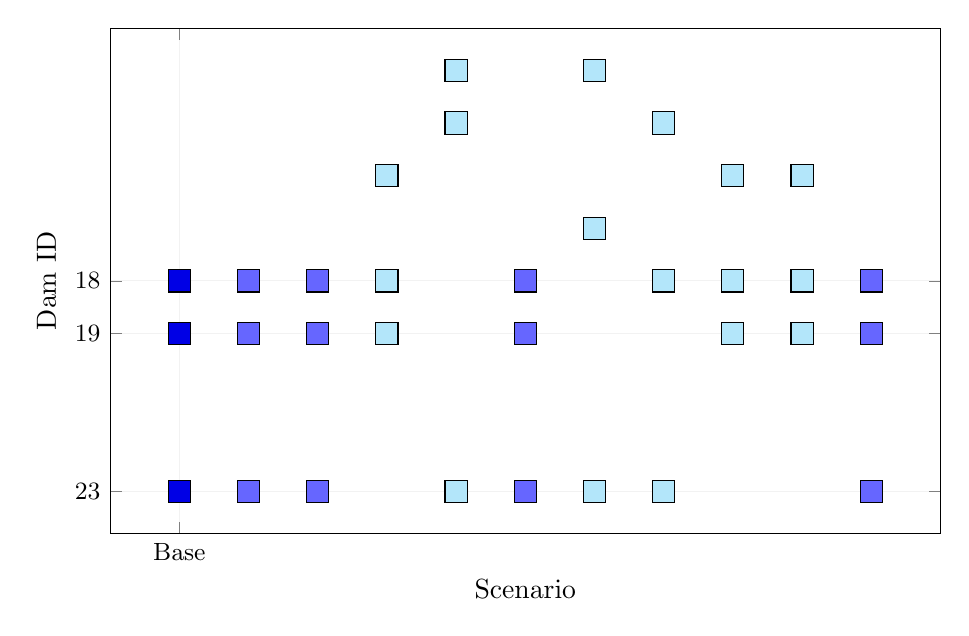
\begin{tikzpicture}
\begin{axis}[
  width=\textwidth,
  height=8cm,
  xlabel={Scenario},
  ylabel={Dam ID},
  xtick=data,
  ytick=data,
  symbolic x coords={Base,Test 1,Test 2,Test 3,Test 4,Test 5,Test 6,Test 7,Test 8,Test 9,Test 10},
  symbolic y coords={1,3,12,13,18,19,20,21,23},
  y dir=reverse,
  grid=both,
  grid style={opacity=0.2},
  tick label style={font=\small},
]
% Base (deep blue)
\addplot[
  only marks,
  mark=square*,
  mark size=4pt,
  draw=black,
  fill=blue!90!black
] coordinates {
  (Base,18) (Base,19) (Base,23)
};
% Matching Base selections in other scenarios (blue)
\addplot[
  only marks,
  mark=square*,
  mark size=4pt,
  draw=black,
  fill=blue!60
] coordinates {
  (Test 1,18) (Test 1,19) (Test 1,23)
  (Test 2,18) (Test 2,19) (Test 2,23)
  (Test 5,18) (Test 5,19) (Test 5,23)
  (Test 10,18) (Test 10,19) (Test 10,23)
};
% All other selections (light blue)
\addplot[
  only marks,
  mark=square*,
  mark size=4pt,
  draw=black,
  fill=cyan!30
] coordinates {
  (Test 3,12) (Test 3,18) (Test 3,19)
  (Test 4,1) (Test 4,3) (Test 4,23)
  (Test 6,1) (Test 6,13) (Test 6,23)
  (Test 7,3) (Test 7,18) (Test 7,23)
  (Test 8,12) (Test 8,18) (Test 8,19)
  (Test 9,12) (Test 9,18) (Test 9,19)
};
\end{axis}
\end{tikzpicture}
\caption{Scenario–dam selection map for the base WGP (first column) and ten test sets. Each filled square marks a selected dam site.}
\label{fig:weight_heatmap}
\end{figure}

\begin{figure}[htbp]
\centering
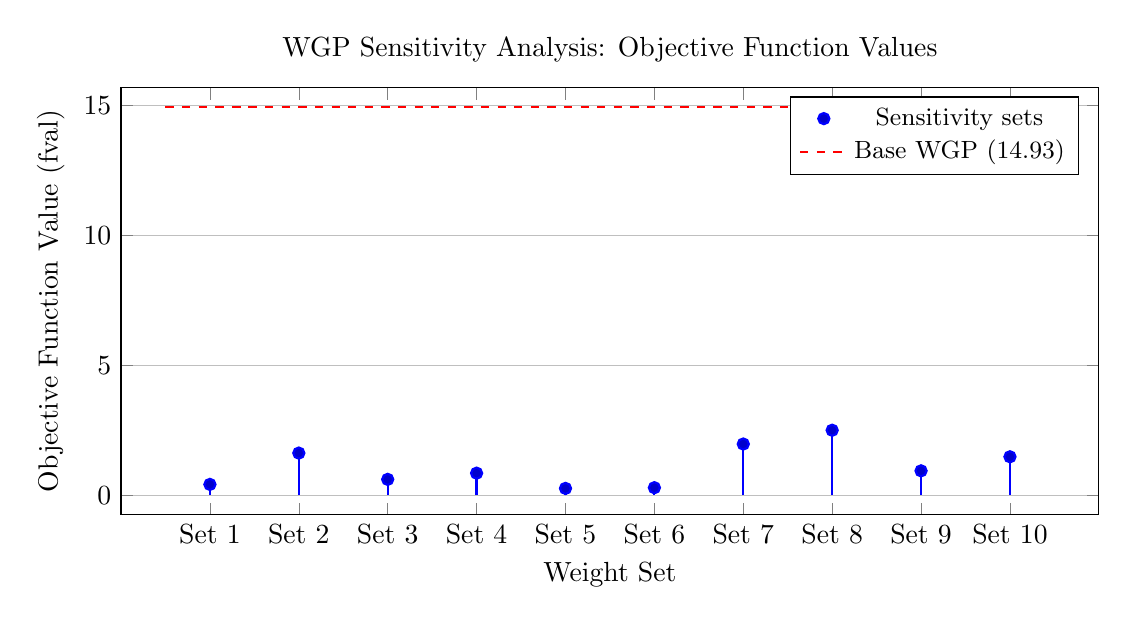
\begin{tikzpicture}
  \begin{axis}[
    title={WGP Sensitivity Analysis: Objective Function Values},
    xlabel={Weight Set},
    ylabel={Objective Function Value (fval)},
    xtick={1,2,3,4,5,6,7,8,9,10},
    xticklabels={Set 1, Set 2, Set 3, Set 4, Set 5, Set 6, Set 7, Set 8, Set 9, Set 10},
    width=14cm,
    height=7cm,
    ymajorgrids,
    ymin=0,
    enlargelimits=0.05,
    legend style={at={(0.98,0.98)},anchor=north east,font=\small},
  ]

  % Lollipop stems
  \addplot+[ycomb, mark=*, thick, blue] coordinates {
    (1,0.4128)
    (2,1.6183)
    (3,0.6062)
    (4,0.845)
    (5,0.2595)
    (6,0.286)
    (7,1.967)
    (8,2.4976)
    (9,0.935)
    (10,1.4761)
  };

  % Base WGP line
  \addplot[red, dashed, thick, domain=0.5:10.5] {14.9277};
  \addlegendentry{Sensitivity sets}
  
  \addlegendentry{Base WGP (14.93)}

  \end{axis}
\end{tikzpicture}
\caption{Lollipop plot of \textit{fval} across 10 weight sets (blue dots), compared with the base Weighted Goal Programming solution (red dashed line).}
\label{fig:wgp_sa_lollipop_fval}
\end{figure}

\begin{figure}[htbp]
\centering
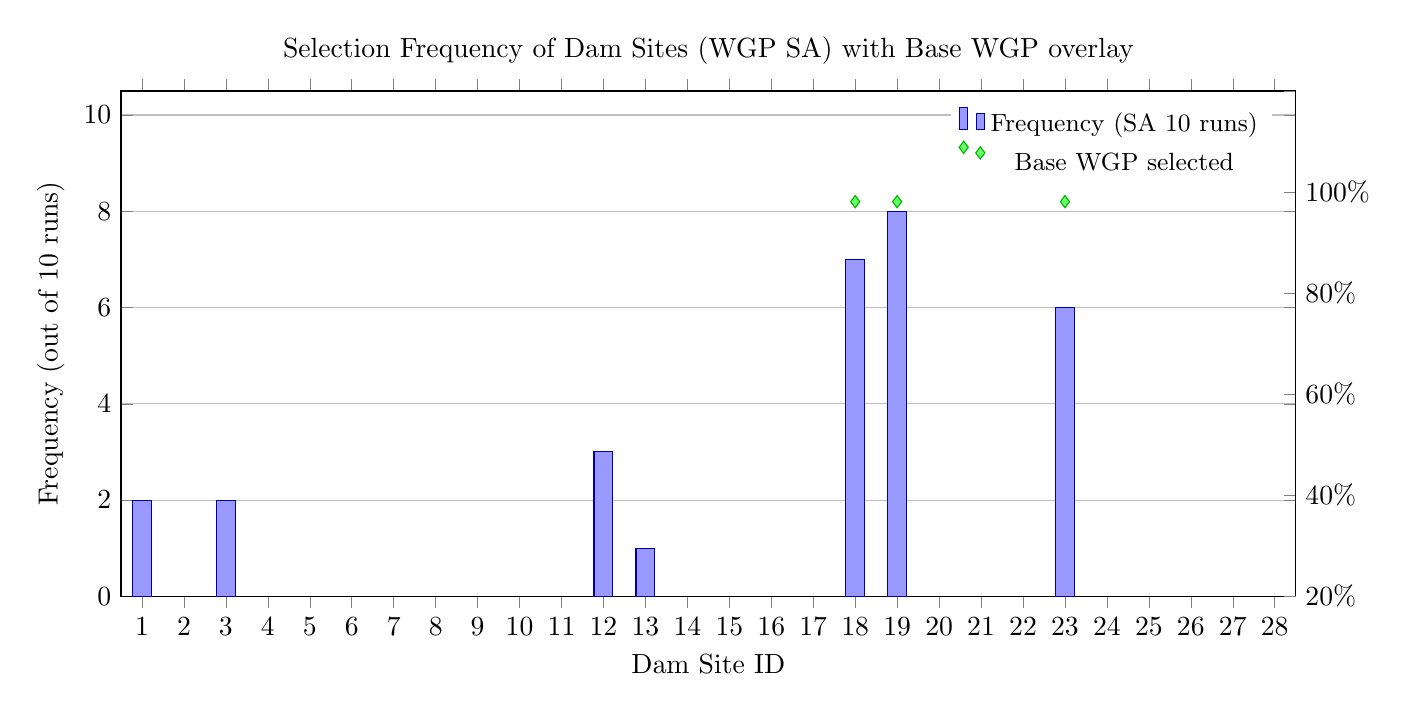
\begin{tikzpicture}

% =======================
% Left axis: Frequency bars (0..10)
% =======================
\begin{axis}[
  title={Selection Frequency of Dam Sites (WGP SA) with Base WGP overlay},
  xlabel={Dam Site ID},
  ylabel={Frequency (out of 10 runs)},
  ymin=0, ymax=10.5,
  xmin=0.5, xmax=28.5,
  xtick={1,2,...,28},
  width=16.5cm, height=8cm,
  ymajorgrids,
  bar width=0.45,
  ybar,
  legend style={font=\small, at={(0.98,0.98)}, anchor=north east, draw=none, fill=white},
]

% --- Frequency bars (hard-coded; 10 SA runs) ---
% Non-zero frequencies:
\addplot+[fill=blue!40!white, draw=blue!70!black] coordinates {
  (1,2) (3,2) (12,3) (13,1) (18,7) (19,8) (23,6)
};
\addlegendentry{Frequency (SA 10 runs)};

% --- Base WGP selections as red diamonds (placed slightly above max) ---
\addplot+[only marks, mark=diamond*, mark size=2.2pt, draw=green!70!black, fill=green!60] coordinates {
  (18,8.2) (19,8.2) (23,8.2)
};
\addlegendentry{Base WGP selected};

\end{axis}

% =======================
% Right axis: Percent labels (0..100%)
% =======================
\begin{axis}[
  hide x axis,
  axis y line*=right,
  ymin=0, ymax=10.5,
  ytick={0,2,4,6,8,10},
  yticklabels={0\%,20\%,40\%,60\%,80\%,100\%},
  width=16.5cm, height=8cm,
]
\end{axis}

\end{tikzpicture}
\caption{Summary of dam-site selection frequency across 10 WGP sensitivity runs; red diamonds mark sites selected by the Base WGP solution. Right axis shows percent of runs.}
\label{fig:wgp_sa_frequency}
\end{figure}
        
\begin{figure}[htbp]
\centering
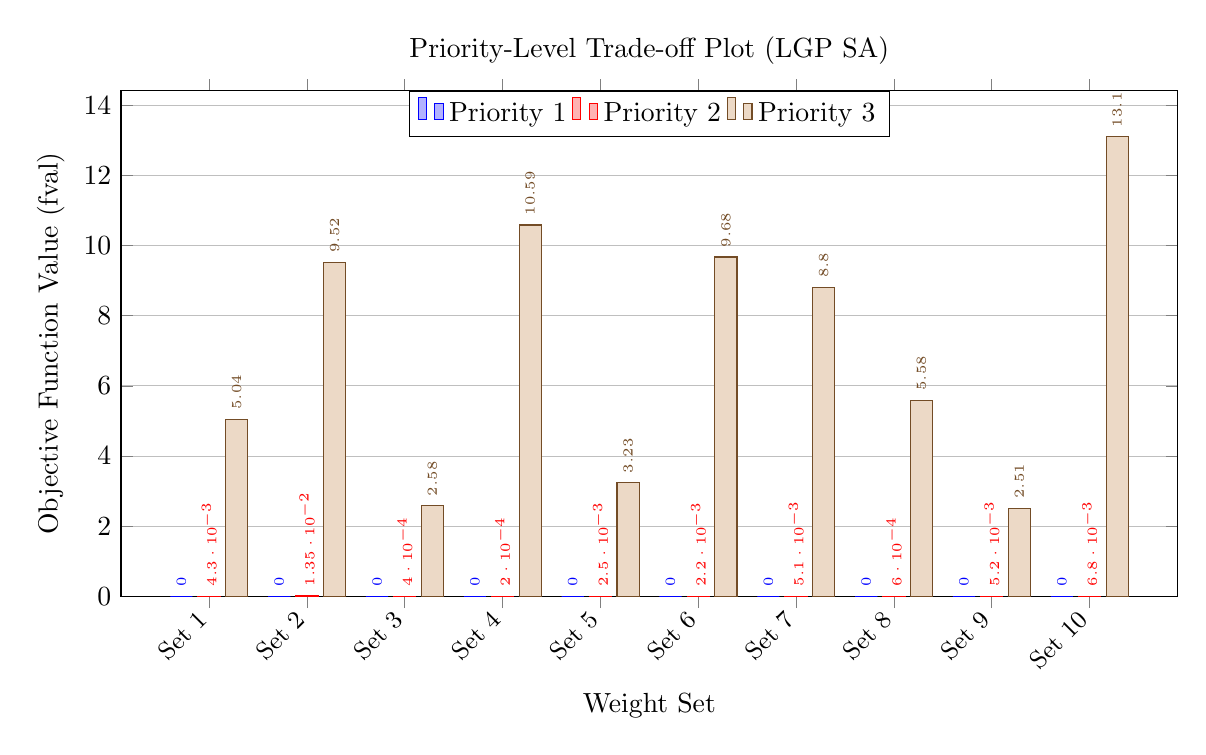
\begin{tikzpicture}
  \begin{axis}[
    ybar,
    bar width=8pt,
    title={Priority-Level Trade-off Plot (LGP SA)},
    xlabel={Weight Set},
    ylabel={Objective Function Value (fval)},
    symbolic x coords={Set 1,Set 2,Set 3,Set 4,Set 5,Set 6,Set 7,Set 8,Set 9,Set 10},
    xtick=data,
    xticklabel style={rotate=45,anchor=east,font=\small},
    width=15cm,
    height=8cm,
    ymin=0,
    enlarge x limits=0.1,
    legend style={at={(0.5,1)},anchor=north,legend columns=3},
    ymajorgrids,
    nodes near coords,
    nodes near coords align={vertical},
    every node near coord/.append style={font=\tiny, rotate=90, anchor=west}
  ]

  % Priority 1 (all zeros)
  \legend{Priority 1, Priority 2, Priority 3}
  \addplot coordinates {(Set 1,0) (Set 2,0) (Set 3,0) (Set 4,0) (Set 5,0) 
                        (Set 6,0) (Set 7,0) (Set 8,0) (Set 9,0) (Set 10,0)};
  % Priority 2
  \addplot coordinates {(Set 1,0.0043) (Set 2,0.0135) (Set 3,0.0004) (Set 4,0.0002) (Set 5,0.0025)
                        (Set 6,0.0022) (Set 7,0.0051) (Set 8,0.0006) (Set 9,0.0052) (Set 10,0.0068)};
  % Priority 3
  \addplot coordinates {(Set 1,5.0425) (Set 2,9.5191) (Set 3,2.5808) (Set 4,10.5879) (Set 5,3.2344)
                        (Set 6,9.6772) (Set 7,8.8018) (Set 8,5.5848) (Set 9,2.5091) (Set 10,13.1004)};

  \end{axis}
\end{tikzpicture}
\caption{Comparison of objective values (\textit{fval}) at Priority 1, 2, and 3 across weight sets for Lexicographic Goal Programming sensitivity analysis. Numbers above bars show exact values.}
\label{fig:lgp_fval_tradeoff}
\end{figure}



\subsubsection{Target Analysis}
The target sensitivity analysis investigated how variations in goal target levels affected model outcomes across the four formulations (WGP, CGP, EGP, and LGP). Figure \ref{fig:target_sa_linechart_with_base} shows the changes in objective values across ten target sets, compared with dashed lines representing the base models. WGP displayed remarkable stability, with values clustered tightly around its base of 14.93. LGP was also comparatively stable, with modest variation between 23 and 38. In contrast, CGP and EGP exhibited wide fluctuations: CGP ranged from 0.0 to 238.5, and EGP from 3.0 to 203.4. The logarithmic scale emphasizes these contrasts, highlighting that while WGP and LGP maintain consistent performance, CGP and EGP are highly sensitive to shifts in target definitions.

These variations are further reflected in dam-site selection patterns. Figure \ref{fig:dam_selection_targets_all_models} compares selected sites across models and target sets, with base solutions included for reference. WGP consistently selected the core set of dams 18, 19, and 20 across all scenarios, reflecting its stability under target perturbations. LGP displayed moderate variability, occasionally switching between site 19, 20, 21, and 28 depending on the target scenario. EGP and CGP were considerably more dynamic, with their selections shifting more frequently across sites such as 1, 16, 19, 20, and 28. This shows that while WGP and LGP preserve a degree of selection robustness, CGP and EGP yield more target-sensitive outcomes that may complicate interpretation and implementation.

Table \ref{tab:target_sa_stats} summarizes the descriptive statistics of objective values across the ten target scenarios for each model. WGP again emerges as the most stable (standard deviation = 0.63), followed by LGP (6.21), while CGP (87.44) and EGP (71.29) show very high variability. Finally, the grouped bar chart in Figure \ref{fig:target_sa_barplot_filtered} presents the frequency of site selection across target sets. The results reinforce the earlier patterns: dams 18–20 are robustly selected by WGP, dam 28 is highly persistent in LGP and partially in CGP/EGP, while sites such as 1, 15, 16, and 22 appear intermittently in the more sensitive models. Taken together, these findings demonstrate that target variation exerts strong influence on CGP and EGP, while WGP and LGP provide more stable recommendations and a clearer distinction between robust and target-sensitive dam sites.

\begin{figure}[htbp]
\centering
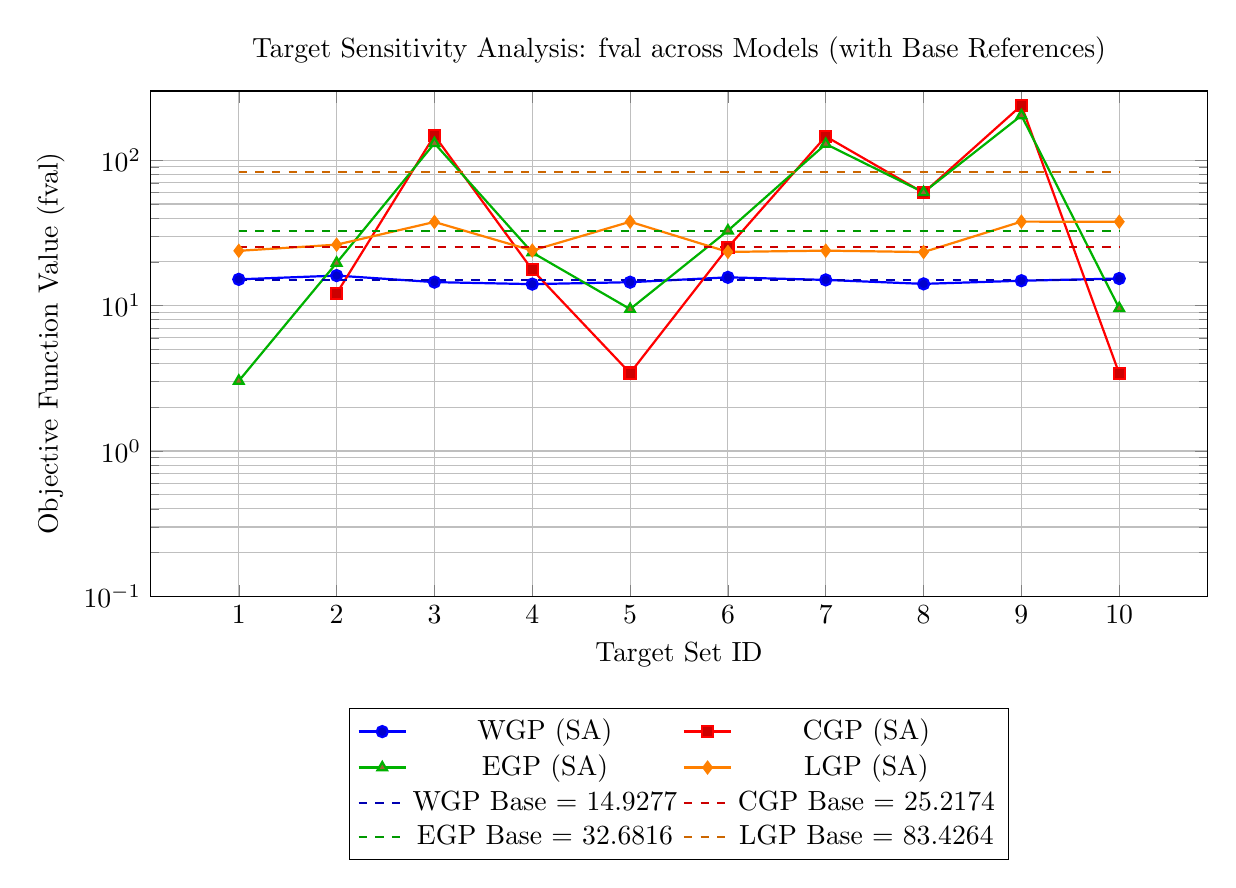
\begin{tikzpicture}
  \begin{axis}[
    title={Target Sensitivity Analysis: fval across Models (with Base References)},
    xlabel={Target Set ID},
    ylabel={Objective Function Value (fval)},
    width=15cm, height=8cm,
    xtick={1,2,...,10},
    ymin=0.1, ymax=300,
    ymode=log, log basis y=10,
    legend style={at={(0.5,-0.22)},anchor=north,legend columns=2},
    grid=both,
  ]

  % --- WGP SA ---
  \addplot+[mark=*,blue,thick] coordinates {
    (1,15.1687) (2,16.0963) (3,14.5178) (4,14.0624) (5,14.4975)
    (6,15.6563) (7,15.033) (8,14.1186) (9,14.8396) (10,15.3641)
  };
  \addlegendentry{WGP (SA)}

  % --- CGP SA ---
  \addplot+[mark=square*,red,thick] coordinates {
    (1,0) (2,12.1215) (3,148.0771) (4,17.6305) (5,3.4348)
    (6,25.1214) (7,145.9941) (8,59.7109) (9,238.5017) (10,3.404)
  };
  \addlegendentry{CGP (SA)}

  % --- EGP SA ---
  \addplot+[mark=triangle*,green!70!black,thick] coordinates {
    (1,3.0337) (2,19.6847) (3,130.949) (4,23.1993) (5,9.4657)
    (6,32.8122) (7,129.3857) (8,60.1762) (9,203.3531) (10,9.5897)
  };
  \addlegendentry{EGP (SA)}

  % --- LGP SA ---
  \addplot+[mark=diamond*,orange,thick] coordinates {
    (1,23.8339) (2,26.2725) (3,37.6495) (4,23.9389) (5,37.7732)
    (6,23.4183) (7,23.9012) (8,23.3668) (9,37.8524) (10,37.7892)
  };
  \addlegendentry{LGP (SA)}

  % --- Base reference lines (horizontal) ---
  % WGP base = 14.9277
  \addplot[blue!70!black, dashed, thick] coordinates {(1,14.9277) (10,14.9277)};
  \addlegendentry{WGP Base = 14.9277}

  % CGP base = 25.2174
  \addplot[red!80!black, dashed, thick] coordinates {(1,25.2174) (10,25.2174)};
  \addlegendentry{CGP Base = 25.2174}

  % EGP base = 32.6816
  \addplot[green!60!black, dashed, thick] coordinates {(1,32.6816) (10,32.6816)};
  \addlegendentry{EGP Base = 32.6816}

  % LGP base = 83.4264
  \addplot[orange!80!black, dashed, thick] coordinates {(1,83.4264) (10,83.4264)};
  \addlegendentry{LGP Base = 83.4264}

  \end{axis}
\end{tikzpicture} 
\caption{Target Sensitivity Analysis: \textit{fval} across target sets for WGP, CGP, EGP, and LGP with dashed lines showing Base model objective values. Logarithmic scale improves joint visibility across models.}
\label{fig:target_sa_linechart_with_base}
\end{figure}
        
\begin{figure}[htbp]
\centering
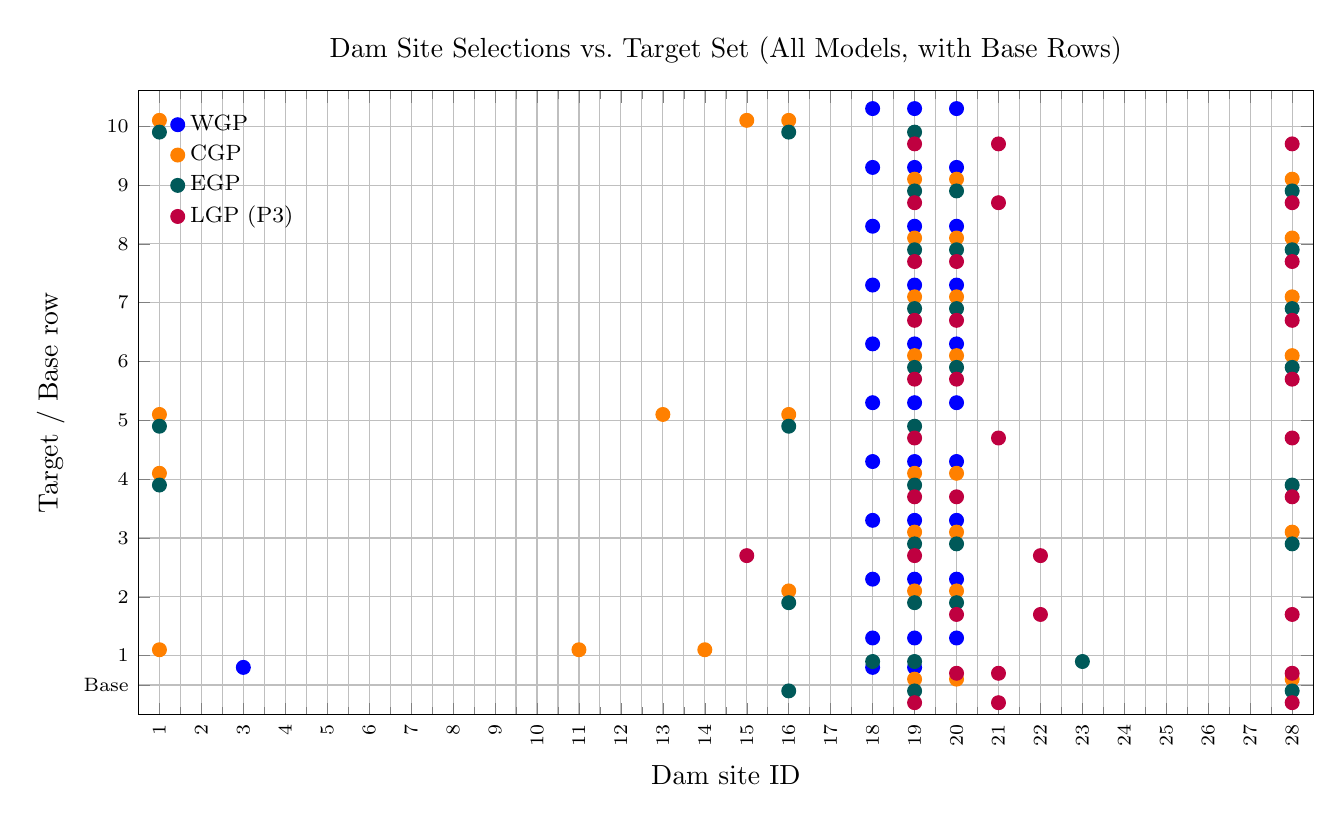
\begin{tikzpicture}
  \begin{axis}[
    title={Dam Site Selections vs.\ Target Set (All Models, with Base Rows)},
    xlabel={Dam site ID},
    ylabel={Target / Base row},
    xmin=0.5, xmax=28.5,
    ymin=0.0, ymax=10.6,
    xtick={1,2,...,28},
    ytick={0.5,1,2,3,4,5,6,7,8,9,10},
    yticklabels={Base,1,2,3,4,5,6,7,8,9,10},
    x tick label style={font=\scriptsize, rotate=90, anchor=east},
    y tick label style={font=\scriptsize},
    width=16.5cm, height=9.5cm,
    grid=both, minor tick num=1,
    legend style={at={(0.02,0.98)}, anchor=north west, draw=none, fill=none, font=\footnotesize},
    legend cell align=left
  ]

  

  % ---- Model row offsets (constant across all targets) ----
  % Base anchor row at y=0.5
  % WGP: +0.30 ; CGP: +0.10 ; EGP: -0.10 ; LGP: -0.30
  % For target set t, rows are: t+0.30 (WGP), t+0.10 (CGP), t-0.10 (EGP), t-0.30 (LGP)

  % ===================== WGP =====================
  \addplot+[only marks, mark=*, mark options={fill=blue, draw=blue}, mark size=2.5pt]
    coordinates
    % --- Base (WGP base selected: 18,19,3) at y=0.5+0.30=0.80
    {(3,0.80) (18,0.80) (19,0.80)
    % --- Target sets (always 18,19,20)
     (18,1.30) (19,1.30) (20,1.30)
     (18,2.30) (19,2.30) (20,2.30)
     (18,3.30) (19,3.30) (20,3.30)
     (18,4.30) (19,4.30) (20,4.30)
     (18,5.30) (19,5.30) (20,5.30)
     (18,6.30) (19,6.30) (20,6.30)
     (18,7.30) (19,7.30) (20,7.30)
     (18,8.30) (19,8.30) (20,8.30)
     (18,9.30) (19,9.30) (20,9.30)
     (18,10.30) (19,10.30) (20,10.30)};
  \addlegendentry{WGP}

  % ===================== CGP =====================
  \addplot+[only marks, mark=*, mark options={fill=orange, draw=orange}, mark size=2.5pt]
    coordinates
    % --- Base (CGP base: 19,20,28) at y=0.5+0.10=0.60
    {(19,0.60) (20,0.60) (28,0.60)
    % --- Target set 1: 1,11,14
     (1,1.10) (11,1.10) (14,1.10)
    % --- 2: 16,19,20
     (16,2.10) (19,2.10) (20,2.10)
    % --- 3: 19,20,28
     (19,3.10) (20,3.10) (28,3.10)
    % --- 4: 1,19,20
     (1,4.10) (19,4.10) (20,4.10)
    % --- 5: 1,13,16
     (1,5.10) (13,5.10) (16,5.10)
    % --- 6: 19,20,28
     (19,6.10) (20,6.10) (28,6.10)
    % --- 7: 19,20,28
     (19,7.10) (20,7.10) (28,7.10)
    % --- 8: 19,20,28
     (19,8.10) (20,8.10) (28,8.10)
    % --- 9: 19,20,28
     (19,9.10) (20,9.10) (28,9.10)
    % --- 10: 1,15,16
     (1,10.10) (15,10.10) (16,10.10)};
  \addlegendentry{CGP}

  % ===================== EGP =====================
  \addplot+[only marks, mark=*, mark options={fill=teal!70!black, draw=teal!70!black}, mark size=2.5pt]
    coordinates
    % --- Base (EGP base: 16,19,28) at y=0.5-0.10=0.40
    {(16,0.40) (19,0.40) (28,0.40)
    % --- 1: 18,19,23
     (18,0.90) (19,0.90) (23,0.90)
    % --- 2: 16,19,20
     (16,1.90) (19,1.90) (20,1.90)
    % --- 3: 19,20,28
     (19,2.90) (20,2.90) (28,2.90)
    % --- 4: 1,19,28
     (1,3.90) (19,3.90) (28,3.90)
    % --- 5: 1,16,19
     (1,4.90) (16,4.90) (19,4.90)
    % --- 6: 19,20,28
     (19,5.90) (20,5.90) (28,5.90)
    % --- 7: 19,20,28
     (19,6.90) (20,6.90) (28,6.90)
    % --- 8: 19,20,28
     (19,7.90) (20,7.90) (28,7.90)
    % --- 9: 19,20,28
     (19,8.90) (20,8.90) (28,8.90)
    % --- 10: 1,16,19
     (1,9.90) (16,9.90) (19,9.90)};
  \addlegendentry{EGP}

  % ===================== LGP (Priority 3) =====================
  \addplot+[only marks, mark=*, mark options={fill=purple, draw=purple}, mark size=2.5pt]
    coordinates
    % --- Base (LGP base P3: 19,21,28) at y=0.5-0.30=0.20
    {(19,0.20) (21,0.20) (28,0.20)
    % --- 1: 20,21,28
     (20,0.70) (21,0.70) (28,0.70)
    % --- 2: 20,22,28
     (20,1.70) (22,1.70) (28,1.70)
    % --- 3: 15,19,22
     (15,2.70) (19,2.70) (22,2.70)
    % --- 4: 19,20,28
     (19,3.70) (20,3.70) (28,3.70)
    % --- 5: 19,21,28
     (19,4.70) (21,4.70) (28,4.70)
    % --- 6: 19,20,28
     (19,5.70) (20,5.70) (28,5.70)
    % --- 7: 19,20,28
     (19,6.70) (20,6.70) (28,6.70)
    % --- 8: 19,20,28
     (19,7.70) (20,7.70) (28,7.70)
    % --- 9: 19,21,28
     (19,8.70) (21,8.70) (28,8.70)
    % --- 10: 19,21,28
     (19,9.70) (21,9.70) (28,9.70)};
  \addlegendentry{LGP (P3)}

  % --- A small guide on offsets (optional)
  \node[anchor=west, font=\scriptsize, align=left] at (axis cs:28.6,10.4)
    {Offsets per target row: \\
     WGP: +0.30,\ CGP: +0.10,\\
     EGP: $-0.10$,\ LGP: $-0.30$.\\
     Base row anchored at 0.5.};
  \end{axis}
\end{tikzpicture}
\caption{Selected dam sites by model and target set (circles; slight vertical offsets prevent overlap). Base models included on the “Base” row.}
\label{fig:dam_selection_targets_all_models}
\end{figure}







\begin{table}[htbp]
\centering
\caption{Descriptive statistics of $fval$ across Target Sensitivity Analysis (per model).}
\label{tab:target_sa_stats}
\begin{tabular}{lcccc}
\toprule
Model & Min & Max & Mean & Std Dev \\
\midrule
WGP & 14.06 & 16.10 & 14.93 & 0.63 \\
CGP & 0.00 & 238.50 & 65.20 & 87.44 \\
EGP & 3.03 & 203.35 & 61.46 & 71.29 \\
LGP (P3) & 23.37 & 37.85 & 29.22 & 6.21 \\
\bottomrule
\end{tabular}
\end{table}


\begin{figure}[htbp]
\centering
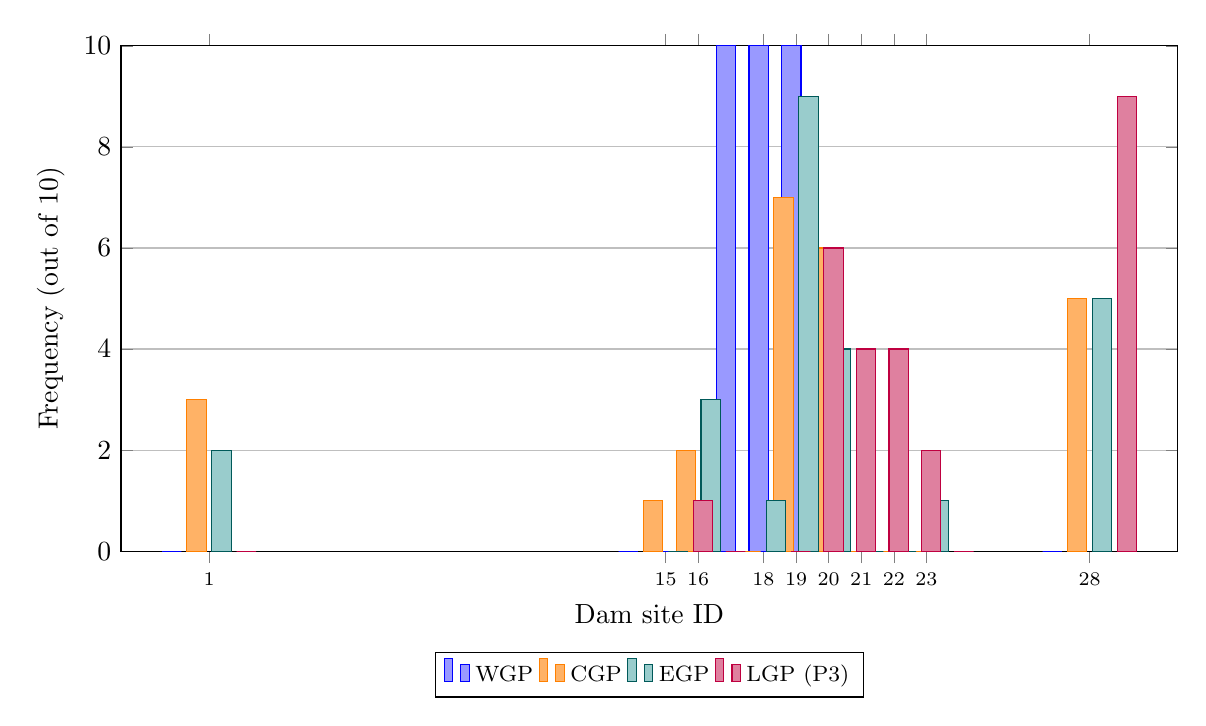
\begin{tikzpicture}
\begin{axis}[
  ybar,
  bar width=7pt,
  width=15cm, height=8cm,
  ylabel={Frequency (out of 10)},
  xlabel={Dam site ID},
  ymin=0, ymax=10,
  xtick=data,
  xticklabel style={font=\scriptsize},
  enlarge x limits=0.1,
  legend style={at={(0.5,-0.2)}, anchor=north, legend columns=4, font=\footnotesize},
  ymajorgrids,
]

% WGP
\addplot+[blue, fill=blue!40] coordinates {
  (1,0) (15,0) (16,0) (18,10) (19,10) (20,10) (21,0) (22,0) (23,0) (28,0)
};

% CGP
\addplot+[orange, fill=orange!60] coordinates {
  (1,3) (15,1) (16,2) (18,0) (19,7) (20,6) (21,0) (22,0) (23,0) (28,5)
};

% EGP
\addplot+[teal!70!black, fill=teal!40] coordinates {
  (1,2) (15,0) (16,3) (18,1) (19,9) (20,4) (21,0) (22,0) (23,1) (28,5)
};

% LGP
\addplot+[purple, fill=purple!50] coordinates {
  (1,0) (15,1) (16,0) (18,0) (19,6) (20,4) (21,4) (22,2) (23,0) (28,9)
};

\legend{WGP, CGP, EGP, LGP (P3)}

\end{axis}
\end{tikzpicture}
\caption{Selection frequency of dam sites across Target Sensitivity Analysis (only sites selected at least once).}
\label{fig:target_sa_barplot_filtered}
\end{figure}









    \section{Discussion}\label{sec:discussion}
Two clear patterns emerge from the experiments a \textit{stable core} of sites that persist across modeling choices and a \textit{flexible margin} whose inclusion depends on policy emphasis.

\paragraph{Stable core: dams 18, 19, and 20.}
These three recur because, taken together, they satisfy complementary benefit goals (maximize) and cost goals (minimize) under the budget and cardinality constraints:
\begin{itemize}
\item \textbf{Dam 18} combines very high rainfall (30.36; benefit~$\uparrow$) with a very small reservoir area (0.02; cost~$\downarrow$). Although its distance to settlement (0.35; benefit~$\uparrow$) and road distance (3.49; cost~$\downarrow$) are not standout, the climate supply plus low inundation footprint make it difficult to dislodge when goals are balanced. The budget cost is modest (157.50).
\item \textbf{Dam 19} is strong on low temperature (16.26; cost~$\downarrow$), very small reservoir area (0.02; cost~$\downarrow$), good rainfall (22.99; benefit~$\uparrow$), and short farm and road distances (0.90 and 0.93; cost~$\downarrow$). Although its distance to settlement (0.81; benefit~$\uparrow$) and farmland area (0.62; benefit~$\uparrow$) are moderate, the overall multi-criterion balance---especially on the cost side---drives repeated selection. The budget cost is modest (158.70).
\item \textbf{Dam 20} combines high rainfall (33.23; benefit~$\uparrow$), low temperature (16.92; cost~$\downarrow$), good farmland area (15.55; benefit~$\uparrow$), and large capacity (62; benefit~$\uparrow$). Distances are mid-range (residence 3.63; farm 2.47; road 1.80), but its supply and land-benefit profile keep it in the set when priorities are hierarchical or balanced. The budget cost is moderate (166.50).
\end{itemize}
Overall, dams 18--20 form a \textit{least-regret set}: even when weights or targets move, there is no single criterion that decisively breaks any of them, and jointly they span climate/resource adequacy (rainfall, capacity), low inundation footprint (small reservoir area for 18--19), and operational feasibility (reasonable access costs), all within budget.

\paragraph{Flexible margin: dams 28, 21, and 23.}
These sites function as \textit{policy levers} that enter when emphasis tilts toward particular social--environmental objectives:
\begin{itemize}
\item \textbf{Dam 28} offers extremely low temperature (15.56; cost~$\downarrow$), tiny reservoir area (0.01; cost~$\downarrow$), high distance to settlement (11.30; benefit~$\uparrow$), and short farm distance (0.93; cost~$\downarrow$). It is weaker on rainfall (7.54) and road distance (3.30; cost~$\downarrow$). It appears when settlement buffers and inundation limits are prioritized over hydrologic supply or when road access is less penalized.
\item \textbf{Dam 21} combines a very small reservoir area (0.01; cost~$\downarrow$), good rainfall (25.07; benefit~$\uparrow$), very high distance to settlement (13.91; benefit~$\uparrow$), and strong farmland area (27.25; benefit~$\uparrow$). Its road distance is large (5.15; cost~$\downarrow$) and farm distance moderate (2.97), so it becomes attractive when social buffers and farmland benefits dominate access costs.
\item \textbf{Dam 23} has outstanding farmland area (91.07; benefit~$\uparrow$) and very short farm distance (0.24; cost~$\downarrow$), making it a natural choice when agricultural benefit is emphasized. Its rainfall (2.53) and distance to settlement (0.24) are low, so it recedes when supply or settlement buffers tighten.
\end{itemize}

\paragraph{Objective values versus robustness}
In the WGP sensitivity experiments, some runs produced numerically smaller objective values than the base (0.26--2.50 versus 14.93).\ref{fig:wgp_sa_lollipop_fval} Since the original WGP was performed with constant weights (1), the observation of smaller objective values, with small deviations in the sensitvity analyses shows that a properly defined weight set could possibly fall reduce the original objective value. On the other hand, because reweighting changes the unit scale of the weighted-sum objective, these values may not directly comparable for overall goodness across runs and may indicate a shift in emphasis. A more interpretable indicator is selection robustness, for example $R = \frac{runs selected}{runs}$: dams 18--20 exceed a reasonable robustness threshold ($R >= 0.6$) , hence the \textit{core} dams 28, 21, and 23 exhibit context-sensitive inclusion, with $R$ rising in scenarios that favor settlement buffers and inundation limits (28, 21) or agricultural benefit (23). In LGP, as expected under lexicographic logic, top-tier priorities stabilize the choice set, while variation appears in lower-tier residuals. \ref{tab:lgpPriorityObjectives}

\paragraph{Practical implication.}
The models do not prescribe a single rigid optimum. They articulate a \textit{decision space} with a stable backbone (18--20) and policy-tunable complements (28, 21, 23). This is advantageous for planning under uncertainty. Decision-makers can commit to the core for baseline resilience and activate the margin to reflect evolving social (settlement buffers), environmental (inundation footprint, temperature), or agricultural (farmland access/area) priorities, without violating budget or feasibility.


% --------------------------------------------
\subsection{Comparison with existing literature}
This study's findings align with several trajectories in the multi-criteria decision-making (MCDM) literature. First, prior surveys document the dominance of value-measurement and outranking approaches (e.g., AHP/ANP, TOPSIS, ELECTRE, PROMETHEE) in infrastructure and siting problems, often implemented with GIS to achieve spatially explicit screening and ranking. These methods have proven effective for structuring criteria hierarchies, eliciting weights, and visualizing trade-offs, and they remain the workhorse in environmental and regional planning applications \cite{ajis2013115,encyclopedia3010006}. In contrast, our work deploys \textit{four} goal programming (GP) formulations on the same decision set, thereby reframing site selection from a single deterministic ranking problem into a family of compromise-seeking models that embody distinct decision logics (balance, priority, fairness, blended) \cite{JonesTamiz2010_PracticalGP}.

Classic distance-to-ideal and outranking approaches are sensitive to weight and threshold settings. Fuzzy and grey extensions were introduced precisely to buffer this sensitivity by representing imprecision in preferences and data \cite{LIANG1999682,MARDANI20154126}. Our results similarly show that model choice and target specification matter, CGP and EGP, which emphasize fairness and blended objective structures, are more reactive to target shifts than WGP and LGP. Rather than adopting fuzzy sets, we operationalize uncertainty via multi-choice goals and explicit sensitivity analyses on both weights and targets. This strategy is consistent with calls in the survey literature to move beyond one-shot rankings toward robustness analysis and scenario exploration \cite{ajis2013115,encyclopedia3010006}.

The GP literature has long argued that satisficing with explicit deviation penalties is well suited to public decisions with competing objectives and hard constraints \cite{JonesTamiz2010_PracticalGP}. Our findings reinforce this view in the dam expansion context. WGP and LGP deliver \textit{stable} recommendations (a persistent core of sites) that are straightforward to communicate, while CGP/EGP surface tension points criteria that become bottlenecks when targets or scales change. This mirrors the theoretical distinction drawn in GP between weighted compromise, lexicographic priority satisfaction, and Chebyshev fairness, and it evidences the practical value of inspecting multiple GP formulations side-by-side rather than privileging a single model.

On criteria design, recent reviews emphasize the shift from purely technical-economic indicators toward sustainability and socio-spatial dimensions in siting (e.g., population exposure/access, land use, proximity/fragmentation), alongside persistent issues of criteria subjectivity and context dependence \cite{KUMAR2017596,Aruldoss2013}. Our criteria set follows this evolution: beyond hydrologic and structural capacity, we incorporate population (normalized), farmland access/area, and proximity to settlements and roads. The observed separation in our results between a stable backbone of sites and a flexible margin is consistent with the literature's observation that a few alternatives often dominate on multiple criteria, while a second tier becomes competitive when social or environmental weights increase \cite{Aruldoss2013}.

With respect to method-reporting practice, several surveys note that many MCDM applications stop at a single configuration without probing robustness, and that transparency about scaling, normalization, and parameter choices is frequently underdeveloped \cite{Aruldoss2013}. We address these concerns by (i) disclosing target construction and normalization; (ii) testing both weight and target perturbations; and (iii) summarizing robustness with selection frequencies (and, where relevant, overlap with the base solution). In this sense, the present study contributes an applied template for multi-model GP analysis with explicit robustness narration. This complements the broader MCDM trajectory toward uncertainty-aware, defensible decision support \cite{jones2010,Mardani2015}.

\subsection{Methodological Contributions}
This study makes three methodological contributions to the field of multi-criteria decision making (MCDM) and infrastructure planning. 

First, by employing four distinct Goal Programming (GP) formulations—Weighted, Lexicographic, Chebyshev, and Extended—the analysis demonstrates how alternative logics of compromise, priority, fairness, and flexibility can be operationalized within a single decision problem. This multi-model perspective moves beyond the dominance of single-method studies in dam planning and highlights the value of comparative modeling \cite{Belton2002,Aruldoss2013}.  

The integration of Multi-Choice Goal Programming (MCGP) into the WGP, CGP, and EGP formulations introduces a novel way of handling uncertainty in socio-technical targets such as population, farmland area, and road access. While earlier dam site studies have applied AHP, TOPSIS, or GIS-based analyses, few have explicitly incorporated flexible aspiration levels. This extension enhances realism by acknowledging that planning targets are rarely fixed and often evolve with policy or stakeholder negotiations.  

Third, the systematic use of sensitivity analysis, both weight and target-based, provides a robustness check that is often underdeveloped in dam site selection literature. By combining Dirichlet-sampled weight perturbations with scenario-based target variations, the study identifies robust core sites while mapping the conditions under which alternative sites gain prominence. This strengthens the credibility of recommendations by ensuring that they hold under a range of plausible assumptions.  

These methodological advances contribute to the broader MCDM literature by illustrating how GP can be adapted for complex, high-stakes water resource decisions in data-scarce and uncertainty-prone contexts such as Morocco.

\subsection{Theoretical Implications}
The findings also carry theoretical implications for the broader field of MCDM.  
By applying four Goal Programming (GP) variants to the same decision problem, the study illustrates how distinct logics of decision-making—balance (WGP), priority (LGP), fairness (CGP), and flexibility (EGP)—can coexist within a unified analytical framework \cite{JonesTamiz2010_PracticalGP}. This reinforces the view that no single MCDM model captures the full complexity of real-world trade-offs \cite{KUMAR2017596,Aruldoss2013}.  

Furthermore, the integration of multi-choice goals and sensitivity testing highlights the importance of treating decision-making as a process under uncertainty rather than a one-off optimization. In this sense, GP models resonate with collective reasoning theories by emphasizing compromise and adaptability over rigid optimality \cite{Borges2020}. Together, these insights position GP not only as a computational tool but also as a conceptual bridge between optimization models and inclusive, deliberative decision processes.

\subsection{Limitations and Future Work}
Despite its contributions, this study has some limitations.  
First, the analysis relies on available hydrological, climatic, and socio-economic datasets that, while comprehensive, may not fully capture ecological constraints such as biodiversity impacts or sedimentation dynamics. Data normalization and target setting, though carefully designed, remain partly subjective and context-dependent, reflecting a common challenge in MCDM applications \cite{Belton2002,Mardani2015}.  

Second, Goal Programming (GP) formulations are linear by design. While this makes them transparent and computationally tractable, real-world dam planning involves non-linear hydrological and ecological processes that may require more advanced hybrid or simulation-based approaches.  

Third, stakeholder preferences were represented indirectly through weights, priorities, and multi-choice targets rather than through participatory elicitation. As such, the models approximate but do not fully capture the deliberative dimension of decision-making.  

Future research should address these limitations by incorporating fuzzy or hybrid GP methods to account for non-linearity and uncertainty, integrating richer ecological and social datasets, and testing participatory frameworks where stakeholders co-define weights and aspiration levels. Extending the analysis to multi-period planning or rehabilitation of existing dams would also enhance policy relevance under climate and budgetary constraints.

\subsection{Closing Synthesis}
In summary, this study demonstrates that Goal Programming (GP) provides a rigorous yet flexible framework for addressing the multi-dimensional challenge of dam site selection in Morocco. By applying four GP variants alongside multi-choice extensions and systematic sensitivity analysis, the research reveals a clear structure of decision outcomes, a stable core of dams (18, 19, 20) that remain robust across models and scenarios, and a flexible margin of alternatives (28, 21, 23) that gain relevance under specific policy emphases.  

This dual structure—stability, when combined with adaptability, highlights the practical value of GP in contexts where policy must balance economic, social, environmental, and technical objectives under uncertainty. The analysis reinforces the view that infrastructure planning should not seek a single rigid optimum, but rather a decision space that accommodates evolving priorities and diverse stakeholder perspectives. Thus, the study advances both the methodological practice of MCDM and its theoretical positioning as a tool for inclusive and robust decision support in complex, resource-constrained environments.






    \section{Chapter 5 - Conclusions}\label{sec:conclusions}
This study applied Goal Programming (GP) to the problem of selecting three optimal dam sites from a set of twenty-eight candidates under multiple, and sometimes conflicting, objectives. GP was chosen because of its ability to balance competing economic, social, environmental, and technical concerns in a structured and transparent way. Unlike single-objective optimization, GP offers multiple formulations that allow decision makers to incorporate their preferences through weighting, prioritization, and fairness-driven rules. Moreover, GP aligns closely with principles of collective intelligence, providing a decision framework that accommodates diverse viewpoints and contextual constraints while still generating actionable recommendations.  

To fully explore the dam site selection problem, four GP variants were employed, each addressing a distinct sub-question. The Weighted Goal Programming (WGP) model asked: what is the most balanced solution when all objectives are weighted simultaneously? The Lexicographic Goal Programming (LGP) model investigated: what solution emerges when objectives are ranked by strict priority? The Chebyshev Goal Programming (CGP) model examined: what solution minimizes the maximum deviation, thereby ensuring fairness across objectives? Finally, the Extended Goal Programming (EGP) model explored: how do solutions change when large deviations are penalized more heavily, revealing asymmetric trade-offs? Together, these formulations ensured that the problem was analyzed not from a single viewpoint, but across different logics of compromise, priority, fairness, and flexibility.

Multi-choice decision making (MCDM) was applied specifically to five selected targets: population, residence distance, farmland distance, nearest road, and farmland area. These criteria were identified as the most critical socio-technical and environmental considerations from earlier screening of possible objectives. Focusing on these five allowed for a tractable yet comprehensive representation of the competing goals most relevant to dam placement. The purpose of using MCDM here was not only to reveal the trade-offs between these key targets, but also to compare how different GP models interpret and resolve these trade-offs, thereby supporting more transparent decision making.

Sensitivity analysis was then conducted in two parts to test both the robustness and the reliability of the results. Weight sensitivity analysis examined how solutions shifted when the relative importance of objectives was perturbed, revealing which dam sites were consistently robust (selected across many scenarios) and which were sensitive to weight changes. Target sensitivity analysis, in contrast, evaluated the models under changing target levels, demonstrating that while WGP and LGP were stable, CGP and EGP displayed greater variability. These experiments were designed not only to test model stability, but also to guide decision makers by highlighting which recommendations remain credible even under uncertainty.

The combined findings suggest that dams 18, 19,  and 20 form a consistently robust core set, appearing frequently across models and scenarios. However, a more nuanced recommendation emerges from the sensitivity results: while these three sites are highly reliable, site 28 and, to a lesser extent, sites 21 and 23, emerge as meaningful alternatives when particular objectives—especially environmental or social priorities—are given greater weight. Thus, the final recommendation is not a single rigid solution, but a set of robust core dams (18, 19, 20) complemented by flexible alternatives (28, 21, 23) that can be emphasized depending on contextual preferences. This flexibility, supported by GP and sensitivity analysis, strengthens the decision-making process by balancing stability with adaptability to local policy and stakeholder priorities.

Beyond the specific case of dam site selection, this study demonstrates the broader value of Goal Programming in infrastructure planning under competing objectives. By combining multiple GP formulations with systematic sensitivity analysis, the research illustrates how quantitative models can be translated into robust yet flexible recommendations that accommodate diverse stakeholder priorities. This integration of MCDM with sensitivity testing thus strengthens the link between optimization models and practical, policy-relevant decision support.

    \clearpage

    % \printbibliography
    \bibliography{mybibfile}

    \clearpage

    \appendix

\section{Appendix}\label{sec:appendix}

\subsection{Dam site data for 28 dams}

\begin{table}[htbp]
\centering
\caption{Generated weight sets (Dirichlet distribution, each row sums to 1).}
\label{tab:sa_weights}
\resizebox{\textwidth}{!}{%
\begin{tabular}{c|cccccccccc}
\toprule
Set & $w_1$ & $w_2$ & $w_3$ & $w_4$ & $w_5$ & $w_6$ & $w_7$ & $w_8$ & $w_9$ & $w_{10}$ \\
\midrule
1 & 0.0227 & 0.2049 & 0.0468 & 0.0386 & 0.0914 & 0.1428 & 0.0317 & 0.0192 & 0.1159 & 0.2860 \\
2 & 0.0070 & 0.0021 & 0.2364 & 0.2445 & 0.0683 & 0.0274 & 0.0969 & 0.0971 & 0.0131 & 0.2071 \\
3 & 0.3275 & 0.0069 & 0.0260 & 0.2038 & 0.0424 & 0.0671 & 0.1081 & 0.0326 & 0.0850 & 0.1005 \\
4 & 0.0105 & 0.0838 & 0.0079 & 0.3567 & 0.0266 & 0.2107 & 0.0415 & 0.1638 & 0.0694 & 0.0289 \\
5 & 0.0607 & 0.0295 & 0.0513 & 0.3088 & 0.2222 & 0.2819 & 0.0153 & 0.0097 & 0.0114 & 0.0090 \\
6 & 0.2207 & 0.1851 & 0.0263 & 0.0184 & 0.0677 & 0.0660 & 0.0039 & 0.0995 & 0.1187 & 0.1935 \\
7 & 0.1901 & 0.1284 & 0.0442 & 0.0541 & 0.1202 & 0.0061 & 0.0897 & 0.2419 & 0.0414 & 0.0839 \\
8 & 0.0695 & 0.0101 & 0.1077 & 0.1322 & 0.0502 & 0.1241 & 0.2275 & 0.1591 & 0.0325 & 0.0871 \\
9 & 0.0046 & 0.0247 & 0.0449 & 0.0054 & 0.0365 & 0.0569 & 0.2021 & 0.0515 & 0.1027 & 0.4708 \\
10 & 0.0033 & 0.0038 & 0.1642 & 0.3134 & 0.0262 & 0.1393 & 0.1262 & 0.0696 & 0.0527 & 0.1012 \\
\bottomrule
\end{tabular}}
\end{table}


\begin{table}[htbp]
\centering
\caption{Generated RHS target sets (±20\% variation around base values).}
\label{tab:sa_targets}
\resizebox{\textwidth}{!}{%
\begin{tabular}{c|cccccccccc}
\toprule
Set & $t_1$ & $t_2$ & $t_3$ & $t_4$ & $t_5$ & $t_6$ & $t_7$ & $t_8$ & $t_9$ & $t_{10}$ \\
\midrule
1 & 48.6331 & 2.6354 & 0.0417 & 53.4186 & 0.5878 & 17.7502 & 1.7689 & 0.2817 & 0.2283 & 0.8106 \\
2 & 56.0241 & 3.1042 & 0.0351 & 50.8542 & 0.5699 & 24.9478 & 1.4959 & 0.3043 & 0.2024 & 0.6750 \\
3 & 46.6565 & 3.5760 & 0.0414 & 42.8169 & 0.5426 & 24.1885 & 2.1025 & 0.2574 & 0.2187 & 0.5985 \\
4 & 41.3687 & 2.9781 & 0.0477 & 50.4336 & 0.4568 & 23.0273 & 2.0385 & 0.3617 & 0.1850 & 0.6467 \\
5 & 44.6968 & 2.6406 & 0.0397 & 58.0982 & 0.5381 & 19.3880 & 1.9407 & 0.3507 & 0.2600 & 0.5469 \\
6 & 37.8005 & 2.8530 & 0.0352 & 48.3838 & 0.6198 & 22.8369 & 1.6340 & 0.3339 & 0.2521 & 0.7687 \\
7 & 53.1286 & 2.4128 & 0.0380 & 42.9002 & 0.5162 & 26.3075 & 1.9246 & 0.2811 & 0.2400 & 0.7453 \\
8 & 51.5116 & 3.3912 & 0.0322 & 46.3516 & 0.4577 & 21.9087 & 2.2171 & 0.3311 & 0.2020 & 0.7095 \\
9 & 49.0387 & 3.2880 & 0.0452 & 39.1999 & 0.4945 & 19.4257 & 1.8464 & 0.3814 & 0.2380 & 0.5974 \\
10 & 41.2884 & 3.1301 & 0.0438 & 55.0954 & 0.4182 & 20.9885 & 1.6371 & 0.3177 & 0.2742 & 0.7036 \\
\bottomrule
\end{tabular}}
\end{table}


\begin{table}[htbp]
\centering
\caption{Generated budget and number-of-sites sets.}
\label{tab:sa_budget_n_k}
\begin{tabular}{c|c|c}
\toprule
Set & Budget & $K$ (sites) \\
\midrule
1 & 432.44 & 3 \\
2 & 584.80 & 2 \\
3 & 524.80 & 3 \\
4 & 563.68 & 4 \\
5 & 417.06 & 3 \\
6 & 501.52 & 5 \\
7 & 488.04 & 2 \\
8 & 542.47 & 2 \\
9 & 447.02 & 4 \\
10 & 470.27 & 5 \\
\bottomrule
\end{tabular}
\end{table}


\begin{landscape}
\begin{table}[htbp]
\centering
\caption{Criteria and budget data for 28 dam sites}
\label{tab:damData}
% \resizebox{\textwidth}{!}{%
\begin{tabular}{c
                S[table-format=3.2]
                S[table-format=3.2]
                S[table-format=2.2]
                S[table-format=2.2]
                S[table-format=2.2]
                S[table-format=2.2]
                S[table-format=2.2]
                S[table-format=2.2]
                S[table-format=2.2]
                S[table-format=3.2]
                S[table-format=3.1]}
\toprule
Dam & {Height} & {Capacity} & {Res.~Area} & {Temp.} & {Pop.} & {Rainfall} & {Residence} & {Farm.~Dist.} & {Nearest~Road} & {Farm.~Area} & {Budget} \\
\midrule
1  & 29.00 & 2.00   & 0.08 & 18.94 & 0.24 & 15.98 & 3.52 & 0.10 & 0.01 & 226.95 & 163.4 \\
2  & 33.00 & 18.00  & 0.24 & 18.75 & 0.38 & 17.45 & 11.65& 1.29 & 0.21 & 214.26 & 170.9 \\
3  & 71.00 & 96.00  & 0.60 & 19.06 & 0.24 & 10.80 & 0.70 & 0.11 & 0.25 & 6.02   & 158.2 \\
4  & 50.00 & 83.00  & 0.88 & 19.10 & 21.80& 13.32 & 3.58 & 3.63 & 0.01 & 36.19  & 180.9 \\
5  & 40.00 & 9.50   & 0.26 & 18.94 & 0.28 & 15.98 & 4.08 & 1.69 & 0.11 & 60.24  & 168.6 \\
6  & 46.00 & 13.00  & 0.07 & 18.00 & 0.23 & 19.57 & 2.97 & 5.11 & 1.12 & 0.13   & 174.8 \\
7  & 18.00 & 2.00   & 0.08 & 18.78 & 0.13 & 12.29 & 2.50 & 2.75 & 0.23 & 0.05   & 167.3 \\
8  & 64.00 & 725.00 & 20.00& 18.98 & 0.14 & 17.02 & 15.76& 2.90 & 0.02 & 23.57  & 192.5 \\
9  & 100.00& 197.00 & 0.50 & 16.30 & 0.51 & 10.47 & 3.20 & 6.35 & 0.01 & 41.94  & 191.2 \\
10 & 85.00 & 369.00 & 1.90 & 17.50 & 0.57 & 12.15 & 7.82 & 0.16 & 2.82 & 21.81  & 180.3 \\
11 & 20.00 & 2.70   & 0.08 & 16.38 & 0.00 & 11.52 & 28.64& 16.80& 5.69 & 0.01   & 193.8 \\
12 & 20.00 & 1.00   & 0.29 & 21.37 & 0.66 & 3.73  & 0.81 & 0.90 & 0.86 & 12.05  & 152.2 \\
13 & 26.00 & 1.30   & 0.02 & 18.98 & 0.20 & 17.19 & 3.91 & 0.33 & 0.83 & 16.21  & 156.8 \\
14 & 17.00 & 1.00   & 0.03 & 18.42 & 0.19 & 19.19 & 2.60 & 3.24 & 0.28 & 31.09  & 166.0 \\
15 & 15.00 & 1.10   & 0.03 & 18.00 & 50.00& 19.57 & 9.72 & 0.11 & 0.83 & 36.08  & 153.2 \\
16 & 15.00 & 2.30   & 0.07 & 18.00 & 50.00& 19.57 & 6.61 & 0.26 & 0.21 & 36.08  & 154.8 \\
17 & 45.00 & 43.00  & 0.33 & 18.00 & 5.12 & 19.57 & 3.58 & 0.35 & 4.98 & 12.80  & 169.2 \\
18 & 29.00 & 1.00   & 0.02 & 19.29 & 0.40 & 30.36 & 0.35 & 1.77 & 3.49 & 2.09   & 157.5 \\
19 & 57.00 & 6.50   & 0.02 & 16.26 & 0.45 & 22.99 & 0.81 & 0.90 & 0.93 & 0.62   & 158.7 \\
20 & 55.00 & 62.00  & 0.43 & 16.92 & 1.27 & 33.23 & 3.63 & 2.47 & 1.80 & 15.55  & 166.5 \\
21 & 40.00 & 1.00   & 0.01 & 18.95 & 0.31 & 25.07 & 13.91& 2.97 & 5.15 & 27.25  & 164.3 \\
22 & 36.00 & 12.00  & 0.31 & 14.70 & 0.23 & 25.41 & 9.59 & 8.20 & 0.55 & 8.79   & 177.4 \\
23 & 17.00 & 2.00   & 0.05 & 18.54 & 0.83 & 16.42 & 2.53 & 0.24 & 1.46 & 91.07  & 165.3 \\
24 & 55.00 & 55.50  & 0.34 & 16.92 & 0.21 & 33.23 & 2.95 & 5.47 & 2.31 & 0.01   & 169.5 \\
25 & 70.00 & 592.00 & 4.76 & 16.67 & 1.53 & 7.88  & 14.84& 8.13 & 0.29 & 21.96  & 186.7 \\
26 & 94.00 & 216.00 & 0.75 & 21.27 & 0.19 & 9.31  & 25.23& 3.62 & 0.22 & 1.13   & 191.9 \\
27 & 79.00 & 110.00 & 0.51 & 17.40 & 0.68 & 8.07  & 3.86 & 0.58 & 1.26 & 33.78  & 190.4 \\
28 & 26.00 & 3.00   & 0.01 & 15.56 & 0.37 & 7.54  & 11.30& 0.93 & 3.30 & 8.54   & 172.1 \\
\bottomrule
\end{tabular}
% }
\end{table}
\end{landscape}
\begin{landscape}
\begin{table}[htbp]
\centering
\caption{Model Evaluation Results and Selected Sites}
\resizebox{1.4\textwidth}{!}{% <-- change 0.9 to 0.8, 0.7 etc. to zoom out more
\begin{tabular}{l c c c c c c c c c c c c c c c c c c c c c l}
\hline
\textbf{Model} & \textbf{fval} & p1 & p2 & p3 & p4 & p5 & p6 & p7 & p8 & p9 & p10 & n1 & n2 & n3 & n4 & n5 & n6 & n7 & n8 & n9 & n10 & \textbf{Selected Sites} \\
\hline
WGP           & 14.9277 & 0 & 0 & 0 & 0 & 0 & 0 & 0 & 0 & 0 & 0 & 56.0 & 6.5 & 0.05 & 5.35 & 1.16 & 47.70 & 1.83 & 2.59 & 5.65 & 93.10 & 17, 18, 22 \\
CGP           & 25.2174 & 0 & 0 & 0 & 0 & 0 & 0 & 0 & 0 & 0 & 0 & 91.0 & 68.5 & 0.42 & 0    & 1.57 & 41.69 & 13.88 & 3.98 & 5.80 & 24.03 & 19, 20, 28 \\
EGP           & 32.6816 & 0 & 0 & 0 & 0 & 0 & 0 & 0 & 0 & 0 & 0 & 51.0 & 8.8  & 0.06 & 1.08 & 50.30 & 28.03 & 16.86 & 1.77 & 4.21 & 44.56 & 17, 19, 28 \\
LGP Priority 1 & 0      & 0 & 0 & 0 & 0 & 0 & 0 & 0 & 0 & 0 & 0 & 46.0 & 13.0 & 0.13 & 7.33 & 0.24 & 40.15 & 3.96 & 9.31 & 4.61 & 1.59 & 6, 7, 18 \\
LGP Priority 2 & 0.0416 & 0 & 0 & 0 & 0 & 0 & 0 & 0 & 0 & 0 & 0 & 76.0 & 7.5  & 0    & 2.03 & 0.61 & 33.53 & 24.16 & 4.48 & 9.15 & 35.73 & 17, 19, 28 \\
LGP Priority 3 & 83.4264 & 0 & 0 & 0 & 0 & 0 & 0 & 0 & 0 & 0 & 0 & 76.0 & 7.5  & 0    & 2.03 & 0.61 & 33.53 & 24.16 & 4.48 & 9.15 & 35.73 & 17, 19, 28 \\
\hline
\end{tabular}}
\label{tab:model_results}
\end{table}
\end{landscape}
\begin{landscape}
\begin{table}[htbp]
\captionof{table}{WGP Weight Sensitivity Analysis Results (with Selected Sites)}
\resizebox{0.9\linewidth}{!}{%
\begin{tabular}{l c c c c c c c c c c c c c c c c c c c c c l}
\hline
\textbf{Weight Test Set} & \textbf{fval} & p1 & p2 & p3 & p4 & p5 & p6 & p7 & p8 & p9 & p10 & n1 & n2 & n3 & n4 & n5 & n6 & n7 & n8 & n9 & n10 & \textbf{Selected Sites} \\
\hline
1  & 0.4128 & 0 & 0 & 0 & 0 & 0 & 0 & 0 & 0 & 0 & 0 & 56.00 & 6.50 & 0.05 & 5.35 & 1.16 & 47.70 & 1.83 & 2.59 & 5.65 & 93.10 & 18, 19, 23 \\
2  & 1.6183 & 0 & 0 & 0 & 0 & 0 & 0 & 0 & 0 & 0 & 0 & 56.00 & 6.50 & 0.05 & 5.35 & 1.16 & 47.70 & 1.83 & 2.59 & 5.65 & 93.10 & 18, 19, 23 \\
3  & 0.6062 & 0 & 0 & 0 & 0 & 0 & 0 & 0 & 0 & 0 & 0 & 59.00 & 5.50 & 0.29 & 8.18 & 0.99 & 35.01 & 0.11 & 3.25 & 5.05 & 14.08 & 12, 18, 19 \\
4  & 0.8450 & 0 & 0 & 0 & 0 & 0 & 0 & 0 & 0 & 0 & 0 & 70.00 & 97.00 & 0.69 & 7.80 & 0.79 & 21.13 & 4.89 & 0.13 & 1.49 & 323.36 & 1, 3, 23 \\
5  & 0.2595 & 0 & 0 & 0 & 0 & 0 & 0 & 0 & 0 & 0 & 0 & 56.00 & 6.50 & 0.05 & 5.35 & 1.16 & 47.70 & 1.83 & 2.59 & 5.65 & 93.10 & 18, 19, 23 \\
6  & 0.2860 & 0 & 0 & 0 & 0 & 0 & 0 & 0 & 0 & 0 & 0 & 25.00 & 2.30 & 0.11 & 7.72 & 0.75 & 27.52 & 8.10 & 0.35 & 2.07 & 333.55 & 1, 13, 23 \\
7  & 1.9670 & 0 & 0 & 0 & 0 & 0 & 0 & 0 & 0 & 0 & 0 & 98.00 & 101.50 & 0.63 & 5.12 & 1.00 & 28.14 & 2.18 & 0.93 & 2.41 & 97.03 & 3, 19, 23 \\
8  & 2.4976 & 0 & 0 & 0 & 0 & 0 & 0 & 0 & 0 & 0 & 0 & 59.00 & 5.50 & 0.29 & 8.18 & 0.99 & 35.01 & 0.11 & 3.25 & 5.05 & 14.08 & 12, 18, 19 \\
9  & 0.9350 & 0 & 0 & 0 & 0 & 0 & 0 & 0 & 0 & 0 & 0 & 59.00 & 5.50 & 0.29 & 8.18 & 0.99 & 35.01 & 0.11 & 3.25 & 5.05 & 14.08 & 12, 18, 19 \\
10 & 1.4761 & 0 & 0 & 0 & 0 & 0 & 0 & 0 & 0 & 0 & 0 & 56.00 & 6.50 & 0.05 & 5.35 & 1.16 & 47.70 & 1.83 & 2.59 & 5.65 & 93.10 & 18, 19, 23 \\
\hline
\end{tabular}}
\label{tab:wgpWeightSAResult}
\end{table}
\end{landscape}

\begin{landscape}
\begin{table}[htbp]
\centering
\caption{Full dataset results with extracted selected sites.}
\resizebox{1.4\textwidth}{!}{%
\begin{tabular}{cccccccccccccccccccccccc}
\toprule
\textbf{Target Test Set} & \textbf{fval} & 
$p_1$ & $p_2$ & $p_3$ & $p_4$ & $p_5$ & $p_6$ & $p_7$ & $p_8$ & $p_9$ & $p_{10}$ & 
$n_1$ & $n_2$ & $n_3$ & $n_4$ & $n_5$ & $n_6$ & $n_7$ & $n_8$ & $n_9$ & $n_{10}$ &
\textbf{Selected Sites} \\
\midrule
1  & 15.1687 & 0 & 0 & 0 & 0 & 0 & 0 & 0 & 0 & 0 & 0 & 54.3669 & 6.8646 & 0.0483 & 0.6714 & 1.0922 & 52.0198 & 1.9211 & 2.6283 & 5.6517 & 92.9694 & \{36, 37, 40\} \\
2  & 16.0963 & 0 & 0 & 0 & 0 & 0 & 0 & 0 & 0 & 0 & 0 & 46.9759 & 6.3958 & 0.0549 & 3.2358 & 1.1101 & 44.8222 & 2.1941 & 2.6057 & 5.6776 & 93.1050 & \{36, 37, 40\} \\
3  & 14.5178 & 0 & 0 & 0 & 0 & 0 & 0 & 0 & 0 & 0 & 0 & 56.3435 & 5.9240 & 0.0486 & 11.2731 & 1.1374 & 45.5815 & 1.5875 & 2.6526 & 5.6613 & 93.1815 & \{36, 37, 40\} \\
4  & 14.0624 & 0 & 0 & 0 & 0 & 0 & 0 & 0 & 0 & 0 & 0 & 61.6313 & 6.5219 & 0.0423 & 3.6564 & 1.2232 & 46.7427 & 1.6515 & 2.5483 & 5.6950 & 93.1333 & \{36, 37, 40\} \\
5  & 14.4975 & 0 & 0 & 0 & 4.0082 & 0 & 0 & 0 & 0 & 0 & 0 & 58.3032 & 6.8594 & 0.0503 & 0 & 1.1419 & 50.3820 & 1.7493 & 2.5593 & 5.6200 & 93.2331 & \{36, 37, 40\} \\
6  & 15.6563 & 0 & 0 & 0 & 0 & 0 & 0 & 0 & 0 & 0 & 0 & 65.1995 & 6.6470 & 0.0548 & 5.7062 & 1.0602 & 46.9331 & 2.0560 & 2.5761 & 5.6279 & 93.0113 & \{36, 37, 40\} \\
7  & 15.0330 & 0 & 0 & 0 & 0 & 0 & 0 & 0 & 0 & 0 & 0 & 49.8714 & 7.0872 & 0.0520 & 11.1898 & 1.1638 & 43.4625 & 1.7654 & 2.6289 & 5.6400 & 93.0347 & \{36, 37, 40\} \\
8  & 14.1186 & 0 & 0 & 0 & 0 & 0 & 0 & 0 & 0 & 0 & 0 & 51.4884 & 6.1088 & 0.0578 & 7.7384 & 1.2223 & 47.8613 & 1.4729 & 2.5789 & 5.6780 & 93.0705 & \{36, 37, 40\} \\
9  & 14.8396 & 0 & 0 & 0 & 0 & 0 & 0 & 0 & 0 & 0 & 0 & 53.9613 & 6.2120 & 0.0448 & 14.8901 & 1.1855 & 50.3443 & 1.8436 & 2.5286 & 5.6420 & 93.1826 & \{36, 37, 40\} \\
10 & 15.3641 & 0 & 0 & 0 & 1.0054 & 0 & 0 & 0 & 0 & 0 & 0 & 61.7116 & 6.3699 & 0.0462 & 0 & 1.2618 & 48.7815 & 2.0529 & 2.5923 & 5.6058 & 93.0764 & \{36, 37, 40\} \\
\bottomrule
\end{tabular}%
}
\label{tab:wgpTargetSAResult}
\end{table}
\end{landscape}

\begin{landscape}
\begin{table}[htbp]
\centering
\caption{Results of budget-based sensitivity analysis with extracted selected sites.}
\resizebox{1.4\textwidth}{!}{%
\begin{tabular}{cccccccccccccccccccccccc}
\toprule
\textbf{Budget} & \textbf{fval} & 
$p_1$ & $p_2$ & $p_3$ & $p_4$ & $p_5$ & $p_6$ & $p_7$ & $p_8$ & $p_9$ & $p_{10}$ &
$n_1$ & $n_2$ & $n_3$ & $n_4$ & $n_5$ & $n_6$ & $n_7$ & $n_8$ & $n_9$ & $n_{10}$ &
\textbf{Selected Sites} \\
\midrule
432.4411 & \multicolumn{21}{c}{\textit{No feasible results}} \\
584.7991 & 14.9277 & 0 & 0 & 0 & 0 & 0 & 0 & 0 & 0 & 0 & 0 & 56.0000 & 6.5000 & 0.0500 & 5.3500 & 1.1600 & 47.7000 & 1.8300 & 2.5900 & 5.6500 & 93.1000 & \{36, 37, 40\} \\
524.7983 & 14.9277 & 0 & 0 & 0 & 0 & 0 & 0 & 0 & 0 & 0 & 0 & 56.0000 & 6.5000 & 0.0500 & 5.3500 & 1.1600 & 47.7000 & 1.8300 & 2.5900 & 5.6500 & 93.1000 & \{36, 37, 40\} \\
563.6782 & 14.9277 & 0 & 0 & 0 & 0 & 0 & 0 & 0 & 0 & 0 & 0 & 56.0000 & 6.5000 & 0.0500 & 5.3500 & 1.1600 & 47.7000 & 1.8300 & 2.5900 & 5.6500 & 93.1000 & \{36, 37, 40\} \\
417.0606 & \multicolumn{21}{c}{\textit{No feasible results}} \\
501.5193 & 14.9277 & 0 & 0 & 0 & 0 & 0 & 0 & 0 & 0 & 0 & 0 & 56.0000 & 6.5000 & 0.0500 & 5.3500 & 1.1600 & 47.7000 & 1.8300 & 2.5900 & 5.6500 & 93.1000 & \{36, 37, 40\} \\
488.0362 & 14.9277 & 0 & 0 & 0 & 0 & 0 & 0 & 0 & 0 & 0 & 0 & 56.0000 & 6.5000 & 0.0500 & 5.3500 & 1.1600 & 47.7000 & 1.8300 & 2.5900 & 5.6500 & 93.1000 & \{36, 37, 40\} \\
542.4664 & 14.9277 & 0 & 0 & 0 & 0 & 0 & 0 & 0 & 0 & 0 & 0 & 56.0000 & 6.5000 & 0.0500 & 5.3500 & 1.1600 & 47.7000 & 1.8300 & 2.5900 & 5.6500 & 93.1000 & \{36, 37, 40\} \\
447.0190 & \multicolumn{21}{c}{\textit{No feasible results}} \\
470.2650 & 18.1079 & 0 & 0 & 0 & 0 & 0 & 0 & 0 & 0 & 0.0000 & 0 & 59.0000 & 5.5000 & 0.2900 & 8.1800 & 0.9900 & 35.0100 & 0.1100 & 3.2500 & 5.0500 & 14.0800 & \{31, 36, 37\} \\
\bottomrule
\end{tabular}%
}
\label{tab:budget_sensitivity_results}
\end{table}
\end{landscape}

\begin{landscape}
\begin{table}[htbp]
\centering
\caption{Results of site selection analysis with extracted selected site indices.}
\resizebox{1.4\textwidth}{!}{%
\begin{tabular}{cccccccccccccccccccccccc}
\toprule
\textbf{No. of Sites Selected} & \textbf{fval} & 
$p_1$ & $p_2$ & $p_3$ & $p_4$ & $p_5$ & $p_6$ & $p_7$ & $p_8$ & $p_9$ & $p_{10}$ &
$n_1$ & $n_2$ & $n_3$ & $n_4$ & $n_5$ & $n_6$ & $n_7$ & $n_8$ & $n_9$ & $n_{10}$ &
\textbf{Selected Sites} \\
\midrule
3 & 14.9277 & 0 & 0 & 0 & 0 & 0 & 0 & 0 & 0 & 0 & 0 & 
56.0000 & 6.5000 & 0.0500 & 5.3500 & 1.1600 & 47.7000 & 1.8300 & 2.5900 & 5.6500 & 93.1000 & 
\{36, 37, 40\} \\

2 & 7.5259 & 0 & 0 & 0 & 13.1900 & 0 & 0 & 0.7000 & 0 & 0 & 0 & 
39.0000 & 4.5000 & 0 & 0 & 0.3300 & 31.2800 & 0 & 2.3500 & 4.1900 & 2.0300 & 
\{36, 37\} \\

1 & 2.0658 & 0 & 0 & 0.0200 & 32.4800 & 0.0700 & 0 & 1.0500 & 0 & 0 & 0.0600 & 
10.0000 & 3.5000 & 0 & 0 & 0 & 0.9200 & 0 & 0.5800 & 0.7000 & 0 & 
\{36\} \\
\bottomrule
\end{tabular}%
}
\label{tab:site_selection_results}
\end{table}
\end{landscape}

\begin{landscape}
\begin{table}[htbp]
\centering
\caption{Results of target analysis showing fval/D, feature values, and extracted selected site indices.}
\resizebox{1.4\textwidth}{!}{%
\begin{tabular}{cccccccccccccccccccccccc}
\toprule
\textbf{Target Test Set} & \textbf{fval/D} &
$p_1$ & $p_2$ & $p_3$ & $p_4$ & $p_5$ & $p_6$ & $p_7$ & $p_8$ & $p_9$ & $p_{10}$ &
$n_1$ & $n_2$ & $n_3$ & $n_4$ & $n_5$ & $n_6$ & $n_7$ & $n_8$ & $n_9$ & $n_{10}$ &
\textbf{Selected Sites} \\
\midrule
1  & 0        & 0 & 0 & 0 & 0 & 0 & 0 & 0 & 0 & 0 & 0 & 15.3669 & 1.4646 & 0.3583 & 4.8914 & 50.3122 & 21.5298 & 12.2811 & 0.8283 & 1.4717 & 274.2694 & \{1, 31, 34\} \\
2  & 12.1215  & 0 & 0 & 0 & 0 & 0 & 0 & 0 & 0 & 0 & 0 & 70.9759 & 67.6958 & 0.4849 & 0.3258 & 51.1501 & 50.8422 & 9.5541 & 3.3257 & 2.7376 & 51.5750 & \{35, 38, 39\} \\
3  & 148.0771 & 0 & 0 & 0 & 0 & 0 & 0 & 0 & 0 & 0 & 0 & 91.3435 & 67.9240 & 0.4186 & 5.9231 & 1.5474 & 39.5715 & 13.6375 & 4.0426 & 5.8113 & 24.1115 & \{37, 38, 45\} \\
4  & 17.6305  & 0 & 0 & 0 & 0 & 0 & 0 & 0 & 0 & 0 & 0 & 70.6313 & 8.5219 & 0.0623 & 0.3264 & 0.6032 & 23.4827 & 13.5915 & 1.5683 & 4.0550 & 235.4633 & \{1, 37, 45\} \\
5  & 3.4348   & 0 & 0 & 0 & 2.1782 & 0 & 0 & 0 & 0 & 0 & 0 & 25.3032 & 2.9594 & 0.1303 & 0 & 49.9019 & 33.3520 & 12.0993 & 0.3393 & 0.7900 & 278.6931 & \{1, 31, 34\} \\
6  & 25.1214  & 0 & 0 & 0 & 0 & 0 & 0 & 0 & 0 & 0 & 0 & 100.1995 & 68.6470 & 0.4248 & 0.3562 & 1.4702 & 40.9231 & 14.1060 & 3.9661 & 5.7779 & 23.9413 & \{37, 38, 45\} \\
7  & 145.9941 & 0 & 0 & 0 & 0 & 0 & 0 & 0 & 0 & 0 & 0 & 84.8714 & 69.0872 & 0.4220 & 5.8398 & 1.5738 & 37.4525 & 13.8154 & 4.0189 & 5.7900 & 23.9647 & \{37, 38, 45\} \\
8  & 59.7109  & 0 & 0 & 0 & 0 & 0 & 0 & 0 & 0 & 0 & 0 & 86.4884 & 68.1088 & 0.4278 & 2.3884 & 1.6323 & 41.8513 & 13.5229 & 3.9689 & 5.8280 & 24.0005 & \{37, 38, 45\} \\
9  & 238.5017 & 0 & 0 & 0 & 0 & 0 & 0 & 0 & 0 & 0 & 0 & 88.9613 & 68.2120 & 0.4148 & 9.5401 & 1.5955 & 44.3343 & 13.8936 & 3.9186 & 5.7920 & 24.1126 & \{37, 38, 45\} \\
10 & 3.4040   & 0 & 0 & 0 & 0.2916 & 0 & 0 & 0 & 0 & 0.0071 & 0 & 17.7116 & 2.2699 & 0.1362 & 0.1362 & 99.8218 & 34.1315 & 18.2129 & 0.1523 & 0.7829 & 298.4064 & \{1, 32, 33\} \\
\bottomrule
\end{tabular}%
}
\label{tab:cgpTargetSAResult}
\end{table}
\end{landscape}

\begin{landscape}
\begin{table}[htbp]
\centering
\caption{CGP Budget Sensitivity Analysis results showing feasible and infeasible solutions with selected site indices.}
\resizebox{1.4\textwidth}{!}{%
\begin{tabular}{ccccccccccccccccccccccc}
\toprule
\textbf{Budget} & \textbf{fval/D} &
$p_1$ & $p_2$ & $p_3$ & $p_4$ & $p_5$ & $p_6$ & $p_7$ & $p_8$ & $p_9$ & $p_{10}$ &
$n_1$ & $n_2$ & $n_3$ & $n_4$ & $n_5$ & $n_6$ & $n_7$ & $n_8$ & $n_9$ & $n_{10}$ &
\textbf{Selected Sites} \\
\midrule
432.4411 & \multicolumn{21}{c}{\textit{No feasible results}} \\
584.7991 & 0 & 0 & 0 & 0 & 0 & 0 & 0 & 0 & 0 & 0 & 0 & 89.0000 & 599.8000 & 5.0000 & 5.8500 & 1.4900 & 18.9800 & 20.9700 & 9.8300 & 1.0000 & 97.7300 & \{24, 32, 44\} \\
524.7983 & 0 & 0 & 0 & 0 & 0 & 0 & 0 & 0 & 0 & 0 & 0 & 96.0000 & 216.0000 & 1.0800 & 12.8400 & 0.5700 & 6.9500 & 27.7000 & 4.3000 & 0.8600 & 239.4500 & \{1, 31, 44\} \\
563.6782 & 0 & 0 & 0 & 0 & 0.0900 & 0 & 0 & 0 & 0 & 0 & 0 & 96.0000 & 217.7000 & 0.8700 & 7.8500 & 0 & 14.7400 & 55.5300 & 20.2000 & 5.6900 & 227.4100 & \{1, 30, 44\} \\
417.0606 & \multicolumn{21}{c}{\textit{No feasible results}} \\
501.5193 & 0 & 0 & 0 & 0 & 0 & 0 & 0 & 0 & 0 & 0 & 0 & 17.0000 & 1.1000 & 0.3600 & 9.5700 & 50.3800 & 17.2100 & 12.1900 & 0.7900 & 1.4700 & 274.4000 & \{1, 31, 34\} \\
488.0362 & 0 & 0 & 0 & 0 & 0 & 0 & 0 & 0 & 0 & 0 & 0 & 17.0000 & 1.1000 & 0.3600 & 9.5700 & 50.3800 & 17.2100 & 12.1900 & 0.7900 & 1.4700 & 274.4000 & \{1, 31, 34\} \\
542.4664 & 0 & 0 & 0 & 0 & 0 & 0 & 0 & 0 & 0 & 0 & 0 & 96.0000 & 216.0000 & 1.0800 & 12.8400 & 0.5700 & 6.9500 & 27.7000 & 4.3000 & 0.8600 & 239.4500 & \{1, 31, 44\} \\
447.0190 & \multicolumn{21}{c}{\textit{No feasible results}} \\
470.2650 & 0 & 0 & 0 & 0 & 0 & 0 & 0 & 0 & 0 & 0 & 0 & 17.0000 & 1.1000 & 0.3600 & 9.5700 & 50.3800 & 17.2100 & 12.1900 & 0.7900 & 1.4700 & 274.4000 & \{1, 31, 34\} \\
\bottomrule
\end{tabular}%
}

\label{tab:cgpBudgetSAResult}
\end{table}
\end{landscape}

\begin{landscape}
\begin{table}[htbp]
\centering
\caption{CGP number of selected sites sensitivity snalysis results}
\resizebox{1.4\textwidth}{!}{%
\begin{tabular}{ccccccccccccccccccccccc}
\toprule
\textbf{Sites Selected} & \textbf{fval/D} &
$p_1$ & $p_2$ & $p_3$ & $p_4$ & $p_5$ & $p_6$ & $p_7$ & $p_8$ & $p_9$ & $p_{10}$ &
$n_1$ & $n_2$ & $n_3$ & $n_4$ & $n_5$ & $n_6$ & $n_7$ & $n_8$ & $n_9$ & $n_{10}$ &
\textbf{Selected Targets} \\
\midrule
3 & 0 & 
0 & 0 & 0 & 0 & 0 & 0 & 0 & 0 & 0 & 0 &
17.0000 & 1.1000 & 0.3600 & 9.5700 & 50.3800 & 17.2100 & 12.1900 & 0.7900 & 1.4700 & 274.4000 &
\{1, 31, 34\} \\
2 & 0 & 
0 & 0 & 0 & 8.5300 & 0.0900 & 0 & 0 & 0 & 0 & 0 &
76.0000 & 215.0000 & 0.7900 & 0 & 0 & 3.2200 & 26.8900 & 3.4000 & 0 & 227.4000 &
\{1, 47\} \\
1 & 0 & 
27.0000 & 2.0000 & 0 & 27.3700 & 0 & 18.3400 & 1.0500 & 0 & 0 & 0 &
0 & 0 & 0.2500 & 0 & 0.1400 & 0 & 0 & 0.5800 & 0.6300 & 11.3700 &
\{31\} \\
\bottomrule
\end{tabular}%
}

\label{tab:cgpSelectionSAResult}
\end{table}
\end{landscape}

\begin{landscape}
\begin{table}[htbp]
\centering
\caption{EGP Sensitivity Analyses results: evaluation of target test sets with feature values and selected site indices.}
\resizebox{1.4\textwidth}{!}{%
\begin{tabular}{cccccccccccccccccccccccc}
\toprule
\textbf{Target Test Set} & \textbf{fval} & \textbf{D} &
$p_1$ & $p_2$ & $p_3$ & $p_4$ & $p_5$ & $p_6$ & $p_7$ & $p_8$ & $p_9$ & $p_{10}$ &
$n_1$ & $n_2$ & $n_3$ & $n_4$ & $n_5$ & $n_6$ & $n_7$ & $n_8$ & $n_9$ & $n_{10}$ &
\textbf{Selected Targets} \\
\midrule
1  & 3.0337   & 0        & 0 & 0 & 0 & 0 & 0 & 0 & 0 & 0 & 0 & 0 & 54.3669 & 6.8646 & 0.0483 & 0.6714 & 1.0922 & 52.0198 & 1.9211 & 2.6283 & 5.6517 & 92.9694 & \{38, 39, 43\} \\
2  & 19.6847  & 12.1215  & 0 & 0 & 0 & 0 & 0 & 0 & 0 & 0 & 0 & 0 & 70.9759 & 67.6958 & 0.4849 & 0.3258 & 51.1501 & 50.8422 & 9.5541 & 3.3257 & 2.7376 & 51.5750 & \{38, 41, 42\} \\
3  & 130.949  & 148.0771 & 0 & 0 & 0 & 0 & 0 & 0 & 0 & 0 & 0 & 0 & 91.3435 & 67.9240 & 0.4186 & 5.9231 & 1.5474 & 39.5715 & 13.6375 & 4.0426 & 5.8113 & 24.1115 & \{39, 40, 48\} \\
4  & 23.1993  & 17.6305  & 0 & 0 & 0 & 0 & 0 & 0 & 0 & 0 & 0 & 0 & 70.6313 & 8.5219 & 0.0623 & 0.3264 & 0.6032 & 23.4827 & 13.5915 & 1.5683 & 4.0550 & 235.4633 & \{1, 39, 48\} \\
5  & 9.4657   & 3.8696   & 0 & 0 & 0 & 4.8982 & 0 & 0 & 0 & 0 & 0 & 0 & 56.3032 & 8.1594 & 0.1303 & 0 & 50.1519 & 39.1520 & 8.9993 & 0.9093 & 0.8900 & 263.1031 & \{1, 37, 40\} \\
6  & 32.8122  & 25.1214  & 0 & 0 & 0 & 0 & 0 & 0 & 0 & 0 & 0 & 0 & 100.1995 & 68.6470 & 0.4248 & 0.3562 & 1.4702 & 40.9231 & 14.1060 & 3.9661 & 5.7779 & 23.9413 & \{39, 40, 48\} \\
7  & 129.3857 & 145.9941 & 0 & 0 & 0 & 0 & 0 & 0 & 0 & 0 & 0 & 0 & 84.8714 & 69.0872 & 0.4220 & 5.8398 & 1.5738 & 37.4525 & 13.8154 & 4.0189 & 5.7900 & 23.9647 & \{39, 40, 48\} \\
8  & 60.1762  & 59.7109  & 0 & 0 & 0 & 0 & 0 & 0 & 0 & 0 & 0 & 0 & 86.4884 & 68.1088 & 0.4278 & 2.3884 & 1.6323 & 41.8513 & 13.5229 & 3.9689 & 5.8280 & 24.0005 & \{39, 40, 48\} \\
9  & 203.3531 & 238.5017 & 0 & 0 & 0 & 0 & 0 & 0 & 0 & 0 & 0 & 0 & 88.9613 & 68.2120 & 0.4148 & 9.5401 & 1.5955 & 44.3343 & 13.8936 & 3.9186 & 5.7920 & 24.1126 & \{39, 40, 48\} \\
10 & 9.5897   & 3.808    & 0 & 0 & 0 & 1.8954 & 0 & 0 & 0 & 0 & 0 & 0 & 59.7116 & 7.6699 & 0.1262 & 0 & 50.2718 & 37.5515 & 9.3029 & 0.9423 & 0.8758 & 262.9464 & \{1, 37, 40\} \\
\bottomrule
\end{tabular}%
}
\label{tab:egpTargetSAResult}
\end{table}
\end{landscape}

\begin{landscape}
\begin{table}[htbp]
\centering
\caption{EGP Budget-constrained Sensitivity Analyses: results of target test sets with feature values and selected site indices.}
\resizebox{1.4\textwidth}{!}{%
\begin{tabular}{ccccccccccccccccccccccccc}
\toprule
\textbf{Target Test Set} & \textbf{Budget} & \textbf{fval} & \textbf{D} &
$p_1$ & $p_2$ & $p_3$ & $p_4$ & $p_5$ & $p_6$ & $p_7$ & $p_8$ & $p_9$ & $p_{10}$ &
$n_1$ & $n_2$ & $n_3$ & $n_4$ & $n_5$ & $n_6$ & $n_7$ & $n_8$ & $n_9$ & $n_{10}$ &
\textbf{Selected Targets} \\
\midrule        
1  & 432.4411 & \multicolumn{23}{c}{\textit{No feasible results}} \\ 
2  & 584.7991 & 2.9855 & 0 & 0 & 0 & 0 & 0 & 0 & 0 & 0 & 0 & 0 & 0 & 56.0000 & 6.5000 & 0.0500 & 5.3500 & 1.1600 & 47.7000 & 1.8300 & 2.5900 & 5.6500 & 93.1000 & \{39, 40, 43\} \\
3  & 524.7983 & 2.9855 & 0 & 0 & 0 & 0 & 0 & 0 & 0 & 0 & 0 & 0 & 0 & 56.0000 & 6.5000 & 0.0500 & 5.3500 & 1.1600 & 47.7000 & 1.8300 & 2.5900 & 5.6500 & 93.1000 & \{39, 40, 43\} \\
4  & 563.6782 & 2.9855 & 0 & 0 & 0 & 0 & 0 & 0 & 0 & 0 & 0 & 0 & 0 & 56.0000 & 6.5000 & 0.0500 & 5.3500 & 1.1600 & 47.7000 & 1.8300 & 2.5900 & 5.6500 & 93.1000 & \{39, 40, 43\} \\
5  & 417.0606 & \multicolumn{23}{c}{\textit{No feasible results}} \\ 
6  & 501.5193 & 2.9855 & 0 & 0 & 0 & 0 & 0 & 0 & 0 & 0 & 0 & 0 & 0 & 56.0000 & 6.5000 & 0.0500 & 5.3500 & 1.1600 & 47.7000 & 1.8300 & 2.5900 & 5.6500 & 93.1000 & \{39, 40, 43\} \\
7  & 488.0362 & 2.9855 & 0 & 0 & 0 & 0 & 0 & 0 & 0 & 0 & 0 & 0 & 0 & 56.0000 & 6.5000 & 0.0500 & 5.3500 & 1.1600 & 47.7000 & 1.8300 & 2.5900 & 5.6500 & 93.1000 & \{39, 40, 43\} \\
8  & 542.4664 & 2.9855 & 0 & 0 & 0 & 0 & 0 & 0 & 0 & 0 & 0 & 0 & 0 & 56.0000 & 6.5000 & 0.0500 & 5.3500 & 1.1600 & 47.7000 & 1.8300 & 2.5900 & 5.6500 & 93.1000 & \{39, 40, 43\} \\
9  & 447.0190 & \multicolumn{23}{c}{\textit{No feasible results}} \\ 
10 & 470.2650 & 3.6216 & 0 & 0 & 0 & 0 & 0 & 0 & 0 & 0 & 0 & 0 & 0 & 59.0000 & 5.5000 & 0.2900 & 8.1800 & 0.9900 & 35.0100 & 0.1100 & 3.2500 & 5.0500 & 14.0800 & \{33, 38, 39\} \\
\bottomrule
\end{tabular}%
}
\label{tab:egpBudgetSAResult}
\end{table}
\end{landscape}

\begin{landscape}
\begin{table}[htbp]
\centering
\caption{EGP number of selected sites sensitivity snalysis results}
\resizebox{1.4\textwidth}{!}{%
\begin{tabular}{cccccccccccccccccccccccc}
\toprule
\textbf{Number of Sites Selected} & \textbf{fval} & \textbf{D} &
$p_1$ & $p_2$ & $p_3$ & $p_4$ & $p_5$ & $p_6$ & $p_7$ & $p_8$ & $p_9$ & $p_{10}$ &
$n_1$ & $n_2$ & $n_3$ & $n_4$ & $n_5$ & $n_6$ & $n_7$ & $n_8$ & $n_9$ & $n_{10}$ &
\textbf{Selected Targets} \\
\midrule
3 & 2.9855 & 0 &
0 & 0 & 0 & 0 & 0 & 0 & 0 & 0 & 0 & 0 &
56.0000 & 6.5000 & 0.0500 & 5.3500 & 1.1600 & 47.7000 & 1.8300 & 2.5900 & 5.6500 & 93.1000 &
\{37, 38, 41\} \\
2 & 1.5052 & 0 &
0 & 0 & 0 & 13.1900 & 0 & 0 & 0.7000 & 0 & 0 & 0 &
39.0000 & 4.5000 & 0 & 0 & 0.3300 & 31.2800 & 0 & 2.3500 & 4.1900 & 2.0300 &
\{37, 38\} \\
1 & 0.4132 & 0 &
0 & 0 & 0.0200 & 32.4800 & 0.0700 & 0 & 1.0500 & 0 & 0 & 0.0600 &
10.0000 & 3.5000 & 0 & 0 & 0 & 0.9200 & 0 & 0.5800 & 0.7000 & 0 &
\{39\} \\
\bottomrule
\end{tabular}%
}
\label{tab:egpSelectionSAResult}
\end{table}
\end{landscape}
\begin{landscape}
\begin{table}[htbp]
\centering
\caption{LGP Target Sensitivity Analysis for Priority 1}
\resizebox{1.4\textwidth}{!}{%
\begin{tabular}{cccccccccccccccccccccccc}
\toprule
\textbf{Target Test Set} & \textbf{fval} &
$p_1$ & $p_2$ & $p_3$ & $p_4$ & $p_5$ & $p_6$ & $p_7$ & $p_8$ & $p_9$ & $p_{10}$ &
$n_1$ & $n_2$ & $n_3$ & $n_4$ & $n_5$ & $n_6$ & $n_7$ & $n_8$ & $n_9$ & $n_{10}$ &
\textbf{Selected Targets} \\
\midrule
1 & 0 &
0 & 0 & 0 & 0 & 0 & 0 & 0 & 0 & 0 & 0 &
45.8166 & 13.3713 & 0.1221 & 12.9312 & 0.1870 & 40.4746 & 3.6656 & 9.3239 & 4.5982 & 1.7038 &
\{26,27,36\} \\
2 & 0 &
0 & 0 & 0 & 1.3995 & 0 & 0 & 0 & 0 & 0 & 0 &
47.8683 & 0.9883 & 0.0750 & 0 & 0.3798 & 43.4016 & 14.9274 & 7.1193 & 8.6500 & 28.6752 &
\{33,36,39\} \\
3 & 0 &
0 & 0 & 0 & 0 & 0 & 0 & 0 & 0 & 0 & 0 &
43.5964 & 13.5022 & 0.1298 & 13.3625 & 0.1367 & 42.6863 & 3.7705 & 9.3147 & 4.5736 & 1.6196 &
\{26,27,36\} \\
4 & 0 &
0 & 0 & 0 & 0 & 0 & 0 & 0 & 0 & 0 & 0 &
42.0429 & 0.8466 & 0.0767 & 8.0898 & 0.3844 & 41.2670 & 15.1138 & 7.1374 & 8.6434 & 28.6024 &
\{33,36,39\} \\
5 & 0 &
0 & 0 & 0 & 0 & 0 & 0 & 0 & 0 & 0 & 0 &
38.5599 & 13.1304 & 0.1280 & 15.4896 & 0.2380 & 42.8816 & 3.5906 & 9.3468 & 4.5866 & 1.6000 &
\{26,27,36\} \\
6 & 0 &
0 & 0 & 0 & 0 & 0 & 0 & 0 & 0 & 0 & 0 &
40.6912 & 0.5251 & 0.0717 & 5.7874 & 0.4071 & 45.5639 & 15.1302 & 7.1064 & 8.6664 & 28.6407 &
\{33,36,39\} \\
7 & 0 &
0 & 0 & 0 & 0 & 0 & 0 & 0 & 0 & 0 & 0 &
41.2119 & 13.0441 & 0.1237 & 9.4485 & 0.2134 & 43.8448 & 3.9527 & 9.3496 & 4.5643 & 1.6681 &
\{26,27,36\} \\
8 & 0 &
0 & 0 & 0 & 0 & 0 & 0 & 0 & 0 & 0 & 0 &
45.4013 & 0.6944 & 0.0706 & 0.5644 & 0.3426 & 44.5213 & 15.2114 & 7.1688 & 8.6685 & 28.5750 &
\{33,36,39\} \\
9 & 0 &
0 & 0 & 0 & 0 & 0 & 0 & 0 & 0 & 0 & 0 &
36.6660 & 13.3448 & 0.1259 & 8.0468 & 0.1577 & 41.1093 & 3.8649 & 9.3636 & 4.6091 & 1.6742 &
\{26,27,36\} \\
10 & 0 &
0 & 0 & 0 & 0 & 0 & 0 & 0 & 0 & 0 & 0 &
45.8171 & 0.4042 & 0.0746 & 3.3146 & 0.3276 & 42.1563 & 14.9808 & 7.1536 & 8.6785 & 28.7073 &
\{33,36,39\} \\
\bottomrule
\end{tabular}%
}
\label{tab:lgpTargetSAResultP1}
\end{table}
\end{landscape}

\begin{landscape}
\begin{table}[htbp]
\centering
\caption{LGP Target Sensitivity Analysis for Priority 2}
\resizebox{1.4\textwidth}{!}{%
\begin{tabular}{cccccccccccccccccccccccc}
\toprule
\textbf{Target Test Set} & \textbf{fval} &
$p_1$ & $p_2$ & $p_3$ & $p_4$ & $p_5$ & $p_6$ & $p_7$ & $p_8$ & $p_9$ & $p_{10}$ &
$n_1$ & $n_2$ & $n_3$ & $n_4$ & $n_5$ & $n_6$ & $n_7$ & $n_8$ & $n_9$ & $n_{10}$ &
\textbf{Selected Targets} \\
\midrule
1 & 8.8884 &
0 & 0 & 0 & 0 & 0 & 0 & 0 & 0 & 0 & 0 &
98.4529 & 68.0613 & 0.4188 & 8.4696 & 1.5337 & 39.5781 & 14.0400 & 3.9841 & 5.8098 & 23.9165 &
\{36,37,46,50\} \\
2 & 0.0142 &
0 & 0 & 0 & 0.3973 & 0 & 0 & 0 & 0 & 0 & 0 &
43.1582 & 8.0757 & 0.0142 & 0 & 50.3904 & 26.4912 & 19.7920 & 1.6475 & 4.8330 & 44.5890 &
\{36,39,42,50\} \\
3 & 0.0063 &
0 & 0 & 0 & 2.3767 & 0 & 0 & 0 & 0 & 0 & 0 &
47.0041 & 1.7995 & 0.0063 & 0 & 0.3442 & 31.5651 & 27.1303 & 3.8794 & 9.0698 & 51.3287 &
\{35,41,47\} \\
4 & 8.1421 &
0 & 0 & 0 & 0 & 0 & 0 & 0 & 0 & 0 & 0 &
91.6040 & 68.6279 & 0.4133 & 7.7288 & 1.4940 & 41.0211 & 14.2032 & 3.9577 & 5.7780 & 24.0885 &
\{36,37,46,50\} \\
5 & 0.0017 &
0 & 0 & 0 & 6.1021 & 0 & 0 & 0 & 0 & 0 & 0 &
80.0436 & 7.5386 & 0.0017 & 0 & 0.6925 & 30.3029 & 24.1036 & 4.5356 & 9.1340 & 35.6649 &
\{36,38,42,47\} \\
6 & 2.4988 &
0 & 0 & 0 & 0 & 0 & 0 & 0 & 0 & 0 & 0 &
86.5026 & 68.7581 & 0.4205 & 2.0783 & 1.4832 & 45.1897 & 13.6080 & 3.9703 & 5.8400 & 23.9826 &
\{36,37,50\} \\
7 & 1.0498 &
0 & 0 & 0 & 0 & 0 & 0 & 0 & 0 & 0 & 0 &
87.7229 & 68.2129 & 0.4234 & 0.6263 & 1.5922 & 38.0077 & 14.1749 & 3.9332 & 5.7930 & 24.1482 &
\{36,37,50\} \\
8 & 4.6095 &
0 & 0 & 0 & 0 & 0 & 0 & 0 & 0 & 0 & 0 &
99.1672 & 68.2908 & 0.4162 & 4.1933 & 1.5767 & 42.6311 & 13.5697 & 4.0307 & 5.7664 & 24.0094 &
\{36,37,50\} \\
9 & 0 &
0 & 0 & 0.0028 & 2.6339 & 0 & 0 & 0 & 0 & 0 & 0 &
74.5754 & 8.0213 & 0 & 0 & 0.6547 & 33.8136 & 24.2393 & 4.4266 & 9.1865 & 35.6306 &
\{36,38,42,47\} \\
10 & 0.007 &
0 & 0 & 0.0028 & 2.6339 & 0 & 0 & 0 & 0 & 0 & 0 &
74.5754 & 8.0213 & 0 & 0 & 0.6547 & 33.8136 & 24.2393 & 4.4266 & 9.1865 & 35.6306 &
\{36,38,42,47\} \\
\bottomrule
\end{tabular}%
}
\label{tab:lgpTargetSAResultP2}
\end{table}
\end{landscape}

\begin{landscape}
\begin{table}[htbp]
\centering
\caption{LGP Target Sensitivity Analysis for Priority 3}
\resizebox{1.4\textwidth}{!}{%
\begin{tabular}{cccccccccccccccccccccccc}
\toprule
\textbf{Target Test Set} & \textbf{fval} &
$p_1$ & $p_2$ & $p_3$ & $p_4$ & $p_5$ & $p_6$ & $p_7$ & $p_8$ & $p_9$ & $p_{10}$ &
$n_1$ & $n_2$ & $n_3$ & $n_4$ & $n_5$ & $n_6$ & $n_7$ & $n_8$ & $n_9$ & $n_{10}$ &
\textbf{Selected Targets} \\
\midrule
1 & 23.8339 &
0 & 0 & 0 & 0 & 0 & 0 & 0 & 0 & 0 & 0 &
90.8166 & 68.8713 & 0.4121 & 5.6012 & 1.5170 & 42.0146 & 13.5856 & 3.9939 & 5.7882 & 24.1438 &
\{36,37,46,50\} \\
2 & 26.2725 &
0 & 0 & 0 & 7.6495 & 0 & 0 & 0 & 0 & 0 & 0 &
83.8683 & 7.4883 & 0.0050 & 0 & 0.6698 & 31.2816 & 24.1874 & 4.4293 & 9.1600 & 35.6952 &
\{36,38,42,47\} \\
3 & 37.6495 &
0 & 0 & 0 & 0 & 0 & 0 & 0 & 0 & 0 & 0 &
63.0429 & 16.4466 & 0.3267 & 0.0298 & 50.2244 & 41.5170 & 18.4738 & 8.8574 & 2.0834 & 44.7024 &
\{35,41,44,47\} \\
4 & 23.9389 &
0 & 0 & 0 & 0 & 0 & 0 & 0 & 0 & 0 & 0 &
83.5599 & 68.6304 & 0.4180 & 8.1596 & 1.5680 & 44.4216 & 13.5106 & 4.0168 & 5.7766 & 24.0400 &
\{36,37,46,50\} \\
5 & 37.7732 &
0 & 0 & 0 & 6.1021 & 0 & 0 & 0 & 0 & 0 & 0 &
80.0436 & 7.5386 & 0.0017 & 0 & 0.6925 & 30.3029 & 24.1036 & 4.5356 & 9.1340 & 35.6649 &
\{36,38,42,47\} \\
6 & 23.4183 &
0 & 0 & 0 & 0 & 0 & 0 & 0 & 0 & 0 & 0 &
86.5026 & 68.7581 & 0.4205 & 2.0783 & 1.4832 & 45.1897 & 13.6080 & 3.9703 & 5.8400 & 23.9826 &
\{36,37,50\} \\
7 & 23.9012 &
0 & 0 & 0 & 0 & 0 & 0 & 0 & 0 & 0 & 0 &
87.7229 & 68.2129 & 0.4234 & 0.6263 & 1.5922 & 38.0077 & 14.1749 & 3.9332 & 5.7930 & 24.1482 &
\{36,37,50\} \\
8 & 23.3668 &
0 & 0 & 0 & 0 & 0 & 0 & 0 & 0 & 0 & 0 &
99.1672 & 68.2908 & 0.4162 & 4.1933 & 1.5767 & 42.6311 & 13.5697 & 4.0307 & 5.7664 & 24.0094 &
\{36,37,50\} \\
9 & 37.8524 &
0 & 0 & 0.0028 & 2.6339 & 0 & 0 & 0 & 0 & 0 & 0 &
74.5754 & 8.0213 & 0 & 0 & 0.6547 & 33.8136 & 24.2393 & 4.4266 & 9.1865 & 35.6306 &
\{36,38,42,47\} \\
10 & 37.7892 &
0 & 0 & 0 & 1.3684 & 0 & 0 & 0 & 0 & 0 & 0 &
69.1277 & 7.4091 & 0.0070 & 0 & 0.5602 & 35.4288 & 24.1839 & 4.4936 & 9.1116 & 35.8378 &
\{36,38,42,47\} \\
\bottomrule
\end{tabular}%
}
\label{tab:lgpTargetSAResultP3}
\end{table}
\end{landscape}

\begin{landscape}
\begin{table}[htbp]
\centering
\caption{LGP Weight Sensitivity Analysis for Priority 1}
\resizebox{1.4\textwidth}{!}{%
\begin{tabular}{cccccccccccccccccccccccc}
\toprule
\textbf{Weight Test Set} & \textbf{fval} &
$p_1$ & $p_2$ & $p_3$ & $p_4$ & $p_5$ & $p_6$ & $p_7$ & $p_8$ & $p_9$ & $p_{10}$ &
$n_1$ & $n_2$ & $n_3$ & $n_4$ & $n_5$ & $n_6$ & $n_7$ & $n_8$ & $n_9$ & $n_{10}$ &
\textbf{Selected Targets} \\
\midrule
1 & 0 &
0 & 0 & 0 & 0 & 0 & 0 & 0 & 0 & 0 & 0 &
15.0000 & 2.3000 & 0.1300 & 7.3300 & 50.0100 & 40.1500 & 7.6000 & 4.4600 & 3.7000 & 37.5400 &
\{31,36,38,41\} \\
2 & 0 &
0 & 0 & 0 & 0 & 0 & 0 & 0 & 0 & 0 & 0 &
46.0000 & 13.0000 & 0.1300 & 7.3300 & 0.2400 & 40.1500 & 3.9600 & 9.3100 & 4.6100 & 1.5900 &
\{28,29,36\} \\
3 & 0 &
0 & 0 & 0 & 0 & 0 & 0 & 0 & 0 & 0 & 0 &
46.0000 & 13.0000 & 0.1300 & 7.3300 & 0.2400 & 40.1500 & 3.9600 & 9.3100 & 4.6100 & 1.5900 &
\{28,29,36\} \\
4 & 0 &
0 & 0 & 0 & 0 & 0 & 0 & 0 & 0 & 0 & 0 &
46.0000 & 13.0000 & 0.1300 & 7.3300 & 0.2400 & 40.1500 & 3.9600 & 9.3100 & 4.6100 & 1.5900 &
\{28,29,36\} \\
5 & 0 &
0 & 0 & 0 & 0 & 0 & 0 & 0 & 0 & 0 & 0 &
46.0000 & 13.0000 & 0.1300 & 7.3300 & 0.2400 & 40.1500 & 3.9600 & 9.3100 & 4.6100 & 1.5900 &
\{28,29,36\} \\
6 & 0 &
0 & 0 & 0 & 0 & 0 & 0 & 0 & 0 & 0 & 0 &
46.0000 & 13.0000 & 0.1300 & 7.3300 & 0.2400 & 40.1500 & 3.9600 & 9.3100 & 4.6100 & 1.5900 &
\{28,29,36\} \\
7 & 0 &
0 & 0 & 0 & 0 & 0 & 0 & 0 & 0 & 0 & 0 &
46.0000 & 13.0000 & 0.1300 & 7.3300 & 0.2400 & 40.1500 & 3.9600 & 9.3100 & 4.6100 & 1.5900 &
\{28,29,36\} \\
8 & 0 &
0 & 0 & 0 & 0 & 0 & 0 & 0 & 0 & 0 & 0 &
46.0000 & 13.0000 & 0.1300 & 7.3300 & 0.2400 & 40.1500 & 3.9600 & 9.3100 & 4.6100 & 1.5900 &
\{28,29,36\} \\
9 & 0 &
0 & 0 & 0 & 0 & 0 & 0 & 0 & 0 & 0 & 0 &
46.0000 & 13.0000 & 0.1300 & 7.3300 & 0.2400 & 40.1500 & 3.9600 & 9.3100 & 4.6100 & 1.5900 &
\{28,29,36\} \\
10 & 0 &
0 & 0 & 0 & 0 & 0 & 0 & 0 & 0 & 0 & 0 &
46.0000 & 13.0000 & 0.1300 & 7.3300 & 0.2400 & 40.1500 & 3.9600 & 9.3100 & 4.6100 & 1.5900 &
\{28,29,36\} \\
\bottomrule
\end{tabular}%
}
\label{tab:lgpWeightSAResultP1}
\end{table}
\end{landscape}

\begin{landscape}
\begin{table}[htbp]
\centering
\caption{LGP Weight Sensitivity Analysis for Priority 2}
\resizebox{1.4\textwidth}{!}{%
\begin{tabular}{cccccccccccccccccccccccc}
\toprule
\textbf{Weight Test Set} & \textbf{fval} &
$p_1$ & $p_2$ & $p_3$ & $p_4$ & $p_5$ & $p_6$ & $p_7$ & $p_8$ & $p_9$ & $p_{10}$ &
$n_1$ & $n_2$ & $n_3$ & $n_4$ & $n_5$ & $n_6$ & $n_7$ & $n_8$ & $n_9$ & $n_{10}$ &
\textbf{Selected Dams} \\
\midrule
1 & 0.0043 &
0 & 0 & 0 & 0 & 0 & 0 & 0 & 0 & 0 & 0 &
76.0000 & 7.5000 & 0 & 2.0300 & 0.6100 & 33.5300 & 24.1600 & 4.4800 & 9.1500 & 35.7300 &
\{3,7,10,28\} \\
2 & 0.0135 &
0 & 0 & 0 & 0 & 0 & 0 & 0 & 0 & 0 & 0 &
76.0000 & 7.5000 & 0 & 2.0300 & 0.6100 & 33.5300 & 24.1600 & 4.4800 & 9.1500 & 35.7300 &
\{3,7,10,28\} \\
3 & 0.0004 &
0 & 0 & 0 & 0 & 0 & 0 & 0 & 0 & 0 & 0 &
76.0000 & 7.5000 & 0 & 2.0300 & 0.6100 & 33.5300 & 24.1600 & 4.4800 & 9.1500 & 35.7300 &
\{3,7,10,28\} \\
4 & 0.0002 &
0 & 0 & 0 & 0 & 0 & 0 & 0 & 0 & 0 & 0 &
76.0000 & 7.5000 & 0 & 2.0300 & 0.6100 & 33.5300 & 24.1600 & 4.4800 & 9.1500 & 35.7300 &
\{3,7,10,28\} \\
5 & 0.0025 &
0 & 0 & 0 & 0 & 0 & 0 & 0 & 0 & 0 & 0 &
76.0000 & 7.5000 & 0 & 2.0300 & 0.6100 & 33.5300 & 24.1600 & 4.4800 & 9.1500 & 35.7300 &
\{3,7,10,28\} \\
6 & 0.0022 &
0 & 0 & 0 & 0 & 0 & 0 & 0 & 0 & 0 & 0 &
76.0000 & 7.5000 & 0 & 2.0300 & 0.6100 & 33.5300 & 24.1600 & 4.4800 & 9.1500 & 35.7300 &
\{3,7,10,28\} \\
7 & 0.0051 &
0 & 0 & 0 & 0 & 0 & 0 & 0 & 0 & 0 & 0 &
76.0000 & 7.5000 & 0 & 2.0300 & 0.6100 & 33.5300 & 24.1600 & 4.4800 & 9.1500 & 35.7300 &
\{3,7,10,28\} \\
8 & 0.0006 &
0 & 0 & 0 & 0 & 0 & 0 & 0 & 0 & 0 & 0 &
76.0000 & 7.5000 & 0 & 2.0300 & 0.6100 & 33.5300 & 24.1600 & 4.4800 & 9.1500 & 35.7300 &
\{3,7,10,28\} \\
9 & 0.0052 &
0 & 0 & 0 & 0 & 0 & 0 & 0 & 0 & 0 & 0 &
76.0000 & 7.5000 & 0 & 2.0300 & 0.6100 & 33.5300 & 24.1600 & 4.4800 & 9.1500 & 35.7300 &
\{3,7,10,28\} \\
10 & 0.0068 &
0 & 0 & 0 & 0 & 0 & 0 & 0 & 0 & 0 & 0 &
76.0000 & 7.5000 & 0 & 2.0300 & 0.6100 & 33.5300 & 24.1600 & 4.4800 & 9.1500 & 35.7300 &
\{3,7,10,28\} \\
\bottomrule
\end{tabular}%
}
\label{tab:lgpWeightSAResultP2}
\end{table}
\end{landscape}

\begin{landscape}
\begin{table}[htbp]
\centering
\caption{LGP Weight Sensitivity Analysis for Priority 3}
\resizebox{1.4\textwidth}{!}{%
\begin{tabular}{cccccccccccccccccccccccc}
\toprule
\textbf{Weight Test Set} & \textbf{fval} &
$p_1$ & $p_2$ & $p_3$ & $p_4$ & $p_5$ & $p_6$ & $p_7$ & $p_8$ & $p_9$ & $p_{10}$ &
$n_1$ & $n_2$ & $n_3$ & $n_4$ & $n_5$ & $n_6$ & $n_7$ & $n_8$ & $n_9$ & $n_{10}$ &
\textbf{Selected Dams} \\
\midrule
1 & 5.0425  & 0 & 0 & 0 & 0 & 0 & 0 & 0 & 0 & 0 & 0 & 76.0000 & 7.5000 & -0.0000 & 2.0300 & 0.6100 & 33.5300 & 24.1600 & 4.4800 & 9.1500 & 35.7300 & \{3,7,10,28\} \\
2 & 9.5191  & 0 & 0 & 0 & 0 & 0 & 0 & 0 & 0 & 0 & 0 & 76.0000 & 7.5000 & -0.0000 & 2.0300 & 0.6100 & 33.5300 & 24.1600 & 4.4800 & 9.1500 & 35.7300 & \{3,7,10,28\} \\
3 & 2.5808  & 0 & 0 & 0 & 0 & 0 & 0 & 0 & 0 & 0 & 0 & 76.0000 & 7.5000 & -0.0000 & 2.0300 & 0.6100 & 33.5300 & 24.1600 & 4.4800 & 9.1500 & 35.7300 & \{3,7,10,28\} \\
4 & 10.5879 & 0 & 0 & 0 & 0 & 0 & 0 & 0 & 0 & 0 & 0 & 76.0000 & 7.5000 & -0.0000 & 2.0300 & 0.6100 & 33.5300 & 24.1600 & 4.4800 & 9.1500 & 35.7300 & \{3,7,10,28\} \\
5 & 3.2344  & 0 & 0 & 0 & 0 & 0 & 0 & 0 & 0 & 0 & 0 & 76.0000 & 7.5000 & -0.0000 & 2.0300 & 0.6100 & 33.5300 & 24.1600 & 4.4800 & 9.1500 & 35.7300 & \{3,7,10,28\} \\
6 & 9.6772  & 0 & 0 & 0 & 0 & 0 & 0 & 0 & 0 & 0 & 0 & 76.0000 & 7.5000 & -0.0000 & 2.0300 & 0.6100 & 33.5300 & 24.1600 & 4.4800 & 9.1500 & 35.7300 & \{3,7,10,28\} \\
7 & 8.8018  & 0 & 0 & 0 & 0 & 0 & 0 & 0 & 0 & 0 & 0 & 76.0000 & 7.5000 & -0.0000 & 2.0300 & 0.6100 & 33.5300 & 24.1600 & 4.4800 & 9.1500 & 35.7300 & \{3,7,10,28\} \\
8 & 5.5848  & 0 & 0 & 0 & 0 & 0 & 0 & 0 & 0 & 0 & 0 & 76.0000 & 7.5000 & -0.0000 & 2.0300 & 0.6100 & 33.5300 & 24.1600 & 4.4800 & 9.1500 & 35.7300 & \{3,7,10,28\} \\
9 & 2.5091  & 0 & 0 & 0 & 0 & 0 & 0 & 0 & 0 & 0 & 0 & 76.0000 & 7.5000 & -0.0000 & 2.0300 & 0.6100 & 33.5300 & 24.1600 & 4.4800 & 9.1500 & 35.7300 & \{3,7,10,28\} \\
10 & 13.1004 & 0 & 0 & 0 & 0 & 0 & 0 & 0 & 0 & 0 & 0 & 76.0000 & 7.5000 & -0.0000 & 2.0300 & 0.6100 & 33.5300 & 24.1600 & 4.4800 & 9.1500 & 35.7300 & \{3,7,10,28\} \\
\bottomrule
\end{tabular}%
}
\label{tab:lgpWeightSensitivityPriority3}
\end{table}
\end{landscape}

\begin{landscape}
\begin{table}[htbp]
\centering
\caption{LGP Budget Sensitivity Analysis Results for Priority 1, showing feasible and infeasible solutions with selected dam indices.}
\resizebox{1.4\textwidth}{!}{%
\begin{tabular}{ccccccccccccccccccccccc}
\toprule
\textbf{Budget} & \textbf{fval} &
$p_1$ & $p_2$ & $p_3$ & $p_4$ & $p_5$ & $p_6$ & $p_7$ & $p_8$ & $p_9$ & $p_{10}$ &
$n_1$ & $n_2$ & $n_3$ & $n_4$ & $n_5$ & $n_6$ & $n_7$ & $n_8$ & $n_9$ & $n_{10}$ &
\textbf{Selected Dams} \\
\midrule
432.4411 & 0 & 0 & 0 & 0 & 0 & 0 & 0 & 0 & 0 & 0 &
20.0000 & 2.7000 & 0.1400 & 5.7100 & 0.0100 & 32.1000 & 29.6300 & 21.0000 & 9.1800 & 1.4700 &
\{27, 31, 37\} \\
584.7991 & 0 & 0 & 0 & 0 & 0 & 0 & 0 & 0 & 0 & 0 &
20.0000 & 2.7000 & 0.1400 & 5.7100 & 0.0100 & 32.1000 & 29.6300 & 21.0000 & 9.1800 & 1.4700 &
\{27, 31, 37\} \\
524.7983 & 0 & 0 & 0 & 0 & 0 & 0 & 0 & 0 & 0 & 0 &
20.0000 & 2.7000 & 0.1400 & 5.7100 & 0.0100 & 32.1000 & 29.6300 & 21.0000 & 9.1800 & 1.4700 &
\{27, 31, 37\} \\
563.6782 & \multicolumn{21}{c}{\textit{No feasible results}} \\
417.0606 & 0 & 0 & 0 & 0 & 0 & 0 & 0 & 0 & 0 & 0 &
54.0000 & 6.8000 & 0.0700 & 4.8100 & 50.3300 & 50.8500 & 5.9100 & 2.6100 & 4.4000 & 38.1100 &
\{36, 38, 39\} \\
501.5193 & \multicolumn{21}{c}{\textit{No feasible results}} \\
488.0362 & 0 & 0 & 0 & 0 & 0 & 0 & 0 & 0 & 0 & 0 &
15.0000 & 2.3000 & 0.1300 & 7.3300 & 50.0100 & 40.1500 & 7.6000 & 4.4600 & 3.7000 & 37.5400 &
\{27, 36, 38\} \\
542.4664 & 0 & 0 & 0 & 0 & 0 & 0 & 0 & 0 & 0 & 0 &
57.0000 & 6.5000 & 0.0800 & 5.5900 & 0.4600 & 43.5700 & 1.8000 & 5.1000 & 4.4200 & 2.0800 &
\{27, 38, 39\} \\
447.0190 & \multicolumn{21}{c}{\textit{No feasible results}} \\
470.2650 & 0 & 0 & 0 & 0 & 0 & 0 & 0 & 0 & 0 & 0 &
20.0000 & 2.7000 & 0.1400 & 5.7100 & 0.0100 & 32.1000 & 29.6300 & 21.0000 & 9.1800 & 1.4700 &
\{27, 31, 37\} \\
\bottomrule
\end{tabular}%
}
\label{tab:lgpBudgetSAResultP1}
\end{table}
\end{landscape}

\begin{landscape}
\begin{table}[htbp]
\centering
\caption{LGP Budget Sensitivity Analysis Results for Priority 2, showing feasible and infeasible solutions with selected dam indices.}
\resizebox{1.4\textwidth}{!}{%
\begin{tabular}{ccccccccccccccccccccccc}
\toprule
\textbf{Budget} & \textbf{fval} &
$p_1$ & $p_2$ & $p_3$ & $p_4$ & $p_5$ & $p_6$ & $p_7$ & $p_8$ & $p_9$ & $p_{10}$ &
$n_1$ & $n_2$ & $n_3$ & $n_4$ & $n_5$ & $n_6$ & $n_7$ & $n_8$ & $n_9$ & $n_{10}$ &
\textbf{Selected Dams} \\
\midrule
432.4411 & 0.0416 & 0 & 0 & 0 & 0 & 0 & 0 & 0 & 0 & 0 & 0 &
76.0000 & 7.5000 & 0 & 2.0300 & 0.6100 & 33.5300 & 24.1600 & 4.4800 & 9.1500 & 35.7300 &
\{39, 41, 48\} \\
584.7991 & 0.0416 & 0 & 0 & 0 & 0 & 0 & 0 & 0 & 0 & 0 & 0 &
76.0000 & 7.5000 & 0 & 2.0300 & 0.6100 & 33.5300 & 24.1600 & 4.4800 & 9.1500 & 35.7300 &
\{39, 41, 48\} \\
524.7983 & 0.0416 & 0 & 0 & 0 & 0 & 0 & 0 & 0 & 0 & 0 & 0 &
76.0000 & 7.5000 & 0 & 2.0300 & 0.6100 & 33.5300 & 24.1600 & 4.4800 & 9.1500 & 35.7300 &
\{39, 41, 48\} \\
563.6782 & \multicolumn{21}{c}{\textit{No feasible results}} \\
417.0606 & 0.6188 & 0 & 0 & 0 & 0 & 0 & 0 & 0 & 0 & 0 & 0 &
65.0000 & 5.8000 & 0.0200 & 5.7900 & 0.5300 & 48.4700 & 3.2100 & 2.6800 & 5.0200 & 18.2400 &
\{31, 36, 37\} \\
501.5193 & \multicolumn{21}{c}{\textit{No feasible results}} \\
488.0362 & 0.0416 & 0 & 0 & 0 & 0 & 0 & 0 & 0 & 0 & 0 & 0 &
76.0000 & 7.5000 & 0 & 2.0300 & 0.6100 & 33.5300 & 24.1600 & 4.4800 & 9.1500 & 35.7300 &
\{39, 41, 48\} \\
542.4664 & 0.3618 & 0 & 0 & 0 & 0 & 0 & 0 & 0 & 0 & 0 & 0 &
76.0000 & 5.8000 & 0.0100 & 5.4500 & 0.4400 & 43.1800 & 16.7700 & 3.8800 & 6.6800 & 43.4000 &
\{31, 36, 38\} \\
447.0190 & \multicolumn{21}{c}{\textit{No feasible results}} \\
470.2650 & 0.0416 & 0 & 0 & 0 & 0 & 0 & 0 & 0 & 0 & 0 & 0 &
76.0000 & 7.5000 & 0 & 2.0300 & 0.6100 & 33.5300 & 24.1600 & 4.4800 & 9.1500 & 35.7300 &
\{39, 41, 48\} \\
\bottomrule
\end{tabular}%
}
\label{tab:lgpBudgetSAResultP2}
\end{table}
\end{landscape}

\begin{landscape}
    \begin{table}[htbp]
     \centering
     \caption{LGP Budget Sensitivity Analysis Results (Priority 3).}
    \resizebox{1.4\textwidth}{!}{%
    \begin{tabular}{ccccccccccccccccccccccc}
        \toprule
        \textbf{Budget} & \textbf{fval} & $p_1$ & $p_2$ & $p_3$ & $p_4$ & $p_5$ & $p_6$ & $p_7$ & $p_8$ & $p_9$ & $p_{10}$ &
        $n_1$ & $n_2$ & $n_3$ & $n_4$ & $n_5$ & $n_6$ & $n_7$ & $n_8$ & $n_9$ & $n_{10}$ & \textbf{Selected Sites} \\
\midrule
432.4411 & 83.4264 & 0 & 0 & 0 & 0 & 0 & 0 & 0 & 0 & 0 & 0 &
76.0000 & 7.5000 & -0.0000 & 2.0300 & 0.6100 & 33.5300 & 24.1600 & 4.4800 & 9.1500 & 35.7300 & \{19, 21, 28\} \\
584.7991 & 83.4264 & \multicolumn{21}{c}{\textit{No feasible results}} \\
524.7983 & 83.4264 & 0 & 0 & 0 & 0 & 0 & 0 & 0 & 0 & 0 & 0 &
76.0000 & 7.5000 & -0.0000 & 2.0300 & 0.6100 & 33.5300 & 24.1600 & 4.4800 & 9.1500 & 35.7300 & \{19, 21, 28\} \\
563.6782 & \multicolumn{21}{c}{\textit{No feasible results}} \\
417.0606 & 6.3617 & 0 & 0 & 0 & 0 & 0 & 0 & 0 & 0 & 0 & 0 &
101.0000 & 100.5000 & 0.8700 & 7.9500 & 0.8300 & 15.4500 & 0.4600 & 1.5900 & 1.8100 & 18.0100 & \{3, 11, 19\} \\
501.5193 & \multicolumn{21}{c}{\textit{No feasible results}} \\
488.0362 & 6.3617 & 0 & 0 & 0 & 0 & 0 & 0 & 0 & 0 & 0 & 0 &
101.0000 & 100.5000 & 0.8700 & 7.9500 & 0.8300 & 15.4500 & 0.4600 & 1.5900 & 1.8100 & 18.0100 & \{3, 11, 19\} \\
542.4664 & 6.3617 & 0 & 0 & 0 & 0 & 0 & 0 & 0 & 0 & 0 & 0 &
101.0000 & 100.5000 & 0.8700 & 7.9500 & 0.8300 & 15.4500 & 0.4600 & 1.5900 & 1.8100 & 18.0100 & \{3, 11, 19\} \\
447.0190 & \multicolumn{21}{c}{\textit{No feasible results}} \\
470.2650 & 6.3617 & 0 & 0 & 0 & 0 & 0 & 0 & 0 & 0 & 0 & 0 &
101.0000 & 100.5000 & 0.8700 & 7.9500 & 0.8300 & 15.4500 & 0.4600 & 1.5900 & 1.8100 & 18.0100 & \{3, 11, 19\} \\
\bottomrule
\end{tabular}%
}
\label{tab:lpgBudgetSAResultP3}
\end{table}
\end{landscape}

\begin{landscape}
\begin{table}[htbp]
\centering
\resizebox{1.4\textwidth}{!}{%
\begin{tabular}{ccccccccccccccccccccccccccccc}
\toprule
\textbf{Model} & \textbf{fval} & \textbf{D} & $z_1$ & $z_2$ & $z_3$ & $z_4$ & $z_5$ &
$p_1$ & $p_2$ & $p_3$ & $p_4$ & $p_5$ & $p_6$ & $p_7$ & $p_8$ & $p_9$ & $p_{10}$ &
$n_1$ & $n_2$ & $n_3$ & $n_4$ & $n_5$ & $n_6$ & $n_7$ & $n_8$ & $n_9$ & $n_{10}$ &
\textbf{Selected Sites} \\
\midrule
WGP & 28.7245 & -- & 1 & 0 & 0 & 0 & 1 &
0 & 0 & 0 & 0 & 0 & 0 & 0 & 0 & 0 & 0 &
56.0000 & 7.5000 & 0.1100 & 5.0000 & 1.0000 & 33.3200 & 4.8100 & 0.8900 & 2.1500 & 317.9600 &
\{1, 19, 23\} \\
CGP & 25.1304 & 25.1304 & 1 & 0 & 0 & 0 & 1 &
0 & 0 & 0 & 1.0052 & 0 & 0 & 0 & 0 & 0 & 0 &
91.0000 & 68.5000 & 0.4200 & 1.0052 & 1.5700 & 41.6900 & 13.6900 & 3.9500 & 5.7800 & 24.0300 &
\{19, 20, 28\} \\
EGP & 32.5462 & 25.1304 & 1 & 0 & 0 & 0 & 1 &
0 & 0 & 0 & 0 & 0 & 0 & 0 & 0 & 0 & 0 &
91.0000 & 68.5000 & 0.4200 & 0.0000 & 1.5700 & 41.6900 & 13.6900 & 3.9500 & 5.7800 & 24.0300 &
\{19, 20, 28\} \\
LGP P1 & 0 & -- & 1 & 0 & 0 & 1 & 0 &
0 & 0 & 0 & 0 & 0 & 0 & 0 & 0 & 0 & 0 &
46.0000 & 13.0000 & 0.1300 & 7.3300 & 0.2400 & 40.1500 & 3.7700 & 9.2800 & 4.5900 & 1.5900 &
\{6, 7, 12\} \\
LGP P2 & 0.0416 & -- & 1 & 0 & 0 & 0 & 1 &
0 & 0 & 0 & 0 & 0 & 0 & 0 & 0 & 0 & 0 &
76.0000 & 7.5000 & 0 & 2.0300 & 0.6100 & 33.5300 & 23.9700 & 4.4500 & 9.1300 & 35.7300 &
\{19, 21, 28\} \\
LGP P3 & 82.7889 & -- & 1 & 0 & 0 & 0 & 1 &
0 & 0 & 0 & 0 & 0 & 0 & 0 & 0 & 0 & 0 &
76.0000 & 7.5000 & 0 & 2.0300 & 0.6100 & 33.5300 & 23.9700 & 4.4500 & 9.1300 & 35.7300 &
\{19, 21, 28\} \\
\bottomrule
\end{tabular}%
}
\caption{Results for WGP, CGP, EGP, and LGP Multi-Choice Goal Programming Extensions.}
\label{tab:mcgpResult}
\end{table}
\end{landscape}



\end{document}